\documentclass{beamer}
\usetheme{metropolis}
\usepackage{graphicx}
\usepackage{subfig}
\usepackage{tcolorbox}
\usepackage{amsmath,mathtools}
\title{Algebra-Based Physics-2: Electricity, Magnetism, and Modern Physics (PHYS135B-01): Unit 5}
\author{Jordan Hanson}
\institute{Whittier College Department of Physics and Astronomy}

\begin{document}
\maketitle

%\section{Summary}
%
%\begin{frame}{Unit 5 Summary}
%\begin{enumerate}
%\item Electromagnetic waves - \textbf{Chapters 24.1 - 24.4}
%\begin{itemize}
%\item Maxwell's Equations
%\item Electromagnetic wave production
%\item Electromagnetic spectrum and energy
%\end{itemize}
%\item Geometric optics - \textbf{Chapters 25.1 - 25.3, 25.6}
%\begin{itemize}
%\item Ray-tracing and reflection
%\item Refraction
%\item Lens optics
%\end{itemize}
%\end{enumerate}
%\end{frame}
%
%\begin{frame}{Unit 5 Summary}
%\begin{enumerate}
%\item Wave optics - \textbf{Chapters 27.1 - 27.3}
%\begin{itemize}
%\item Wave interference
%\item Wave diffraction
%\item Double slit experiments
%\end{itemize}
%\item Nuclear physics in medicine - \textbf{32.1 - 32.4}
%\begin{itemize}
%\item Diagnostics and medical imaging
%\item Biological effects of ionizing radiation
%\item Therapeutic uses of ionizing radiation
%\item Food irradiation
%\end{itemize}
%\end{enumerate}
%\end{frame}
%
%\section{Electromagnetic waves: Maxwell's Equations}
%
%\begin{frame}{Electromagnetic waves: Maxwell's Equations}
%\textbf{\alert{Maxwell's Equations}} are a set of four main ideas describing \textit{the entirety} of electromagnetism.
%\begin{itemize}
%\item \textbf{Electric fields}, or the force per unit test charge, originate on positive charges and terminate on negative charges. The force is related to the permittivity of free space, $\epsilon_0$.  Electric fields give rise to Coulomb's law, or Gauss's law for electricity.
%\item \textbf{Magnetic fields}, or the force per unit test current per unit length, are continuous, having no beginning or end. No magnetic monopoles are known to exist.  The strength of the magnetic force is related to the permeability of free space, $\mu_0$.  Magnetic fields give rise to Gauss's law for magnetism.
%\end{itemize}
%\end{frame}
%
%\begin{frame}{Electromagnetic waves: Maxwell's Equations}
%\textbf{\alert{Maxwell's Equations}} are a set of four main ideas describing \textit{the entirety} of electromagnetism.
%\begin{itemize}
%\item A \textit{changing} \textbf{magnetic field} induces an electromotive force (emf) and, hence, an \textbf{electric field}. The direction of the emf opposes the change.  This is Faraday's law of induction, and includes Lenz's law.
%\item \textbf{Magnetic fields} are generated by \textit{moving charges} (current) or by \textit{changing} \textbf{electric fields}. This is Amp\`{e}re's law, enhanced with the idea that changing \textbf{electric fields} without current or charge induce \textbf{magnetic fields}.
%\end{itemize}
%\end{frame}
%
%\begin{frame}{Electromagnetic waves: Maxwell's Equations}
%Amp\`{e}re's Law is enhanced with the idea that changing \textbf{electric fields} without current or charge induce \textbf{magnetic fields}.
%\begin{figure}
%\centering
%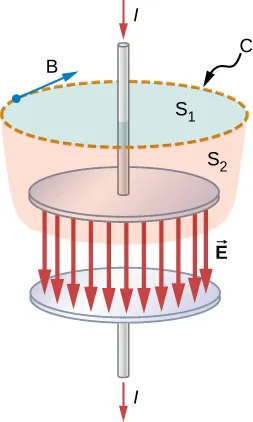
\includegraphics[width=0.275\textwidth]{figures/displacement_current.png}
%\caption{\label{fig:disp_current} When a current creates a B-field, which surface bounding the B-field line is relevant?}
%\end{figure}
%\end{frame}
%
%\begin{frame}{Electromagnetic waves: Maxwell's Equations}
%\small
%The addition to Amp\`{e}re's Law is called \textit{the displacement current}:
%\begin{equation}
%I_{\rm d} = \epsilon_0 \frac{\Delta \Phi_{\rm E}}{\Delta t}
%\end{equation}
%The electric flux is $\Phi_{\rm E} = \vec{E} \cdot \vec{A}$.  Assume we are dealing with surface $S_2$, meaning $I = 0$.  Amp\`{e}re's Law gives
%\begin{align}
%B 2\pi r &= \mu_0\left(I + I_{\rm d}\right) \\
%B 2\pi r &= \mu_0\left(0 + I_{\rm d}\right) \\
%B 2\pi r &= \mu_0\left(\epsilon_0 \frac{\Delta \Phi_E}{\Delta t} \right) = \mu_0\epsilon_0 A\left(\frac{\Delta E}{\Delta t}\right)
%\end{align}
%For a parallel-plate capacitor,
%\begin{equation}
%E = V/d = Q/(Cd) = Qd/(\epsilon_0 A d) = Q/(\epsilon_0 A)
%\end{equation}
%\end{frame}
%
%\begin{frame}{Electromagnetic waves: Maxwell's Equations}
%Insert the magnitude of the E-field into Amp\`{e}re's Law to find:
%\begin{align}
%B 2\pi r &= \mu_0\epsilon_0 A\left(\frac{\Delta E}{\Delta t}\right) \\
%B 2\pi r &= \mu_0\epsilon_0 A \left(\frac{\Delta E}{\epsilon_0 A \Delta t}\right) \\
%B &= \frac{\mu_0}{2\pi r} \frac{\Delta Q}{\Delta t} \\
%\Aboxed{ B &= \frac{\mu_0 I}{2\pi r} }
%\end{align}
%A \textit{changing} \textbf{\alert{E-field}} is responsible for the B-field of a capacitor.
%\end{frame}
%
%\begin{frame}{Electromagnetic waves: Maxwell's Equations}
%What is the B-field generated 1 cm laterally from a capacitor in an RC circuit that charges from 0 to 10 nJ in 1 $\mu$s?
%\begin{itemize}
%\item A: 20 $\mu$T
%\item B: 20 mT
%\item C: 20 nT
%\item D: 20 pT
%\end{itemize}
%\end{frame}
%
%\begin{frame}{Electromagnetic waves: Maxwell's Equations}
%What is the energy stored in the capacitor, if the capacitance is $C = 10$ pF?
%\begin{itemize}
%\item A: 5 $\mu$J
%\item B: 5 mJ
%\item C: 5 nJ
%\item D: 5 pJ
%\end{itemize}
%\small
%Recall that $U = \frac{1}{2} \frac{Q^2}{C}$.
%\end{frame}
%
%\begin{frame}{Electromagnetic waves: Maxwell's Equations}
%\small
%But \textit{where} is the energy stored in a capacitor?  \textbf{The E-field.}  Consider that we proved the stored energy is
%\begin{equation}
%U_{\rm C} = \frac{1}{2} C V^2
%\end{equation}
%The voltage only exists because of the arrangement of charges and the field, and we know that $V = E d$.  Also, the volume is $Ad$.  Thus,
%\begin{align}
%U_{\rm C} &= \frac{1}{2}C E^2 d^2 \\
%U_{\rm C} &= \frac{1}{2}\left(\frac{\epsilon_0 A}{d}\right) E^2 d^2 \\
%\frac{U_{\rm C}}{Ad} &= \frac{1}{2}\epsilon_0 E^2 \\
%\Aboxed{\epsilon_{\rm C} &= \frac{1}{2}\epsilon_0 E^2}
%\end{align}
%\end{frame}
%
%\begin{frame}{Electromagnetic waves: Maxwell's Equations}
%Amp\`{e}re's Law is enhanced with the idea that changing \textbf{electric fields} without current or charge induce \textbf{magnetic fields}.
%\begin{figure}
%\centering
%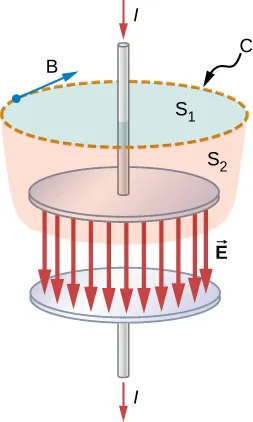
\includegraphics[width=0.275\textwidth]{figures/displacement_current.png}
%\caption{\label{fig:disp_current2} When a current creates a B-field, which surface bounding the B-field line is relevant?}
%\end{figure}
%\end{frame}
%
%\begin{frame}{Electromagnetic waves: Maxwell's Equations}
%What if there was a solenoid inductor $(N = 1)$ next to the capacitor, waiting to catch the B-field and become charged (via Faraday's Law)?  The solenoid will produce some current $I$ to create the \textit{opposite} B-field:
%\begin{align}
%L &= \frac{\mu_0 N^2 A}{d} \\
%U_{\rm L} &= \frac{1}{2} L I^2 \\
%U_{\rm L} &= \frac{1}{2} \frac{\mu_0 A}{d} I^2 \\
%B &= \mu_0 \frac{N}{d} I = \mu_0 \frac{I}{d} \\
%I^2 &= \frac{d^2B^2}{\mu_0^2}
%\end{align}
%\end{frame}
%
%\begin{frame}{Electromagnetic waves: Maxwell's Equations}
%What if there was a solenoid inductor $(N = 1)$ next to the capacitor, waiting to catch the B-field and become charged (via Faraday's Law)?  The solenoid will produce some current $I$ to create the \textit{opposite} B-field:
%\begin{align}
%U_{\rm L} &= \frac{1}{2}\frac{\mu_0 A}{d}\frac{d^2B^2}{\mu_0^2} = \frac{1}{2}\frac{B^2 Ad}{\mu_0} \\
%\frac{U_{\rm L}}{Ad} &= \frac{B^2}{2\mu_0} \\
%\Aboxed{\epsilon_{\rm L} &= \frac{1}{2\mu_0} B^2}
%\end{align}
%Suppose the inductor catches \textit{all} the energy from the capacitor, so that $\epsilon_{\rm C} = \epsilon_{\rm L}$?
%\end{frame}
%
%\begin{frame}{Electromagnetic waves: Maxwell's Equations}
%\small
%If that is true, then
%\begin{align}
%\epsilon_{\rm C} &= \epsilon_{\rm L} \\
%\frac{1}{2}\epsilon_0 E^2 &= \frac{1}{2\mu_0} B^2 \\
%\frac{E}{B} &= \frac{1}{\sqrt{\epsilon_0 \mu_0}}
%\end{align}
%Show that the units of $E/B$ are m s$^{-1}$.  \textit{Hint: recall $F = qE$, and $F = qvB$.}  Knowing that the ratio on the left hand side is a velocity:
%\begin{equation}
%\boxed{v = \frac{1}{\sqrt{\epsilon_0 \mu_0}}} \label{eq:c}
%\end{equation}
%Equation \ref{eq:c} represents the \textbf{\alert{speed of light.}}  Now imagine the inductor charging a second capacitor, and that capacitor charging some second inductor ... the energy starts to propagate.
%\end{frame}
%
%\begin{frame}{Electromagnetic waves: Maxwell's Equations}
%\textbf{\alert{We should be able to observe}} this effect in the lab.  
%\begin{figure}
%\centering
%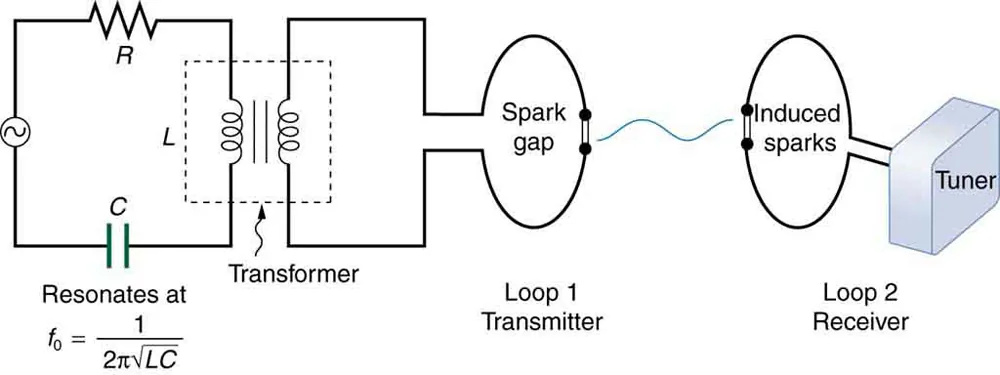
\includegraphics[width=0.7\textwidth]{figures/spark.png}
%\caption{\label{fig:spark} Heinrich Hertz demonstrated the \textit{spark gap} RLC circuit.}
%\end{figure}
%\footnotesize
%\begin{itemize}
%\item The RLC circuit on the left side is set to resonate.
%\item The transformer changes the signal to a high voltage that makes a spark in loop 1.
%\item The RLC circuit in the tuner is set to the same resonance frequency.
%\item Sparks are induced \textit{even though the circuits are not connected with conductors.}
%\end{itemize}
%\end{frame}
%
%\begin{frame}{Electromagnetic waves: Maxwell's Equations}
%\begin{figure}
%\centering
%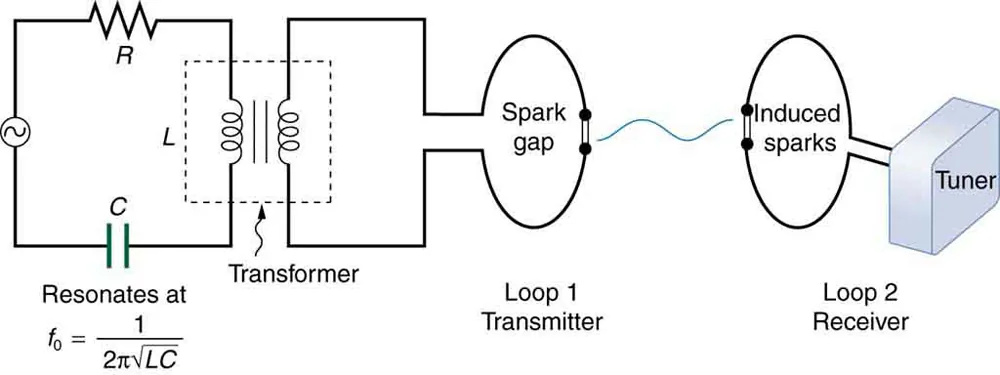
\includegraphics[width=0.5\textwidth]{figures/spark.png}
%\caption{\label{fig:spark2} The transmitter and receiver are connected to RLC circuits with the same resonance frequency.}
%\end{figure}
%If the transmitter and receiver resonance frequency are the same:
%\begin{align}
%f_{\rm L} &= f_{\rm R} \\
%\frac{1}{2\pi \sqrt{L_1 C_1}} &= \frac{1}{2\pi \sqrt{L_2 C_2}} \\
%L_1 C_1 &= L_2 C_2 
%\end{align}
%\end{frame}
%
%\begin{frame}{Electromagnetic waves: Maxwell's Equations}
%If the transmitter and receiver resonance frequency are the same:
%\begin{equation}
%L_{\rm TX} C_{\rm TX} = L_{\rm RX} C_{\rm RX}
%\end{equation}
%If the transmitter (TX) inductance is 1 mH, and the TX capacitance is 0.1 mF, and the receiver (RX) capacitance is 10 mF, what is the RX inductance?
%\begin{itemize}
%\item A: 1 mH
%\item B: 0.1 mH
%\item C: 0.01 mH
%\item D: 0.001 mH
%\end{itemize}
%\footnotesize
%Hint: treat this as a scaling problem.
%\end{frame}
%
%\begin{frame}{Electromagnetic waves: Maxwell's Equations}
%If the transmitter (TX) inductance is 1 mH, and the TX capacitance is 0.1 mF, and the receiver (RX) capacitance is 0.2 mF, what is the RX inductance?
%\begin{itemize}
%\item A: 5 mH
%\item B: 0.5 mH
%\item C: 0.05 mH
%\item D: 0.005 mH
%\end{itemize}
%\footnotesize
%Hint: treat this as a scaling problem.
%\end{frame}
%
%\begin{frame}{Electromagnetic waves: Maxwell's Equations}
%\small
%That electromagnetic fields can \textit{propagate} was strong evidence that they are wavelike.  All waves that obey the ``wave equation'' share a relationship between the speed, $v$, frequency $f$, and the \textit{wavelength} $\lambda$:
%\begin{equation}
%v = f\lambda
%\end{equation}
%The wavelength is the displacement between wave peaks, and $1/f = T$ is the period in time between peaks.  If the speed is $v = 1/\sqrt{\epsilon_0 \mu_0}$, and the resonance frequency corresponds to a capacitance of 0.2 $\mu$F and inductance of 0.5 $\mu$H, what is the wavelength?
%\begin{itemize}
%\item A: 3750 m
%\item B: 375 m
%\item C: 37.5 m
%\item D: 3.75 m
%\end{itemize}
%\end{frame}
%
%\begin{frame}{Electromagnetic waves: Maxwell's Equations}
%If the speed of light is $3 \times 10^{8}$ m/s, what is this same speed in m/ns?
%\begin{itemize}
%\item A: 30 m/ns
%\item B: 3 m/ns
%\item C: 0.3 m/ns
%\item D: 0.03 m/ns
%\end{itemize}
%\end{frame}
%
%\begin{frame}{Electromagnetic waves: Maxwell's Equations}
%What is the frequency of electromagnetic radiation with a wavelength comparable to the length of a person ($\approx 1$ m)?
%\begin{itemize}
%\item A: 0.3 GHz
%\item B: 3 GHz
%\item C: 300 MHz
%\item D: 3000 MHz
%\end{itemize}
%\footnotesize
%Note: is there any reason to expect limitations on the wavelengths and frequencies of electromagnetic waves?
%\end{frame}
%
%\section{Electromagnetic waves: Electromagnetic wave production}
%
%\begin{frame}{Electromagnetic waves: Electromagnetic wave production}
%\begin{figure}
%\centering
%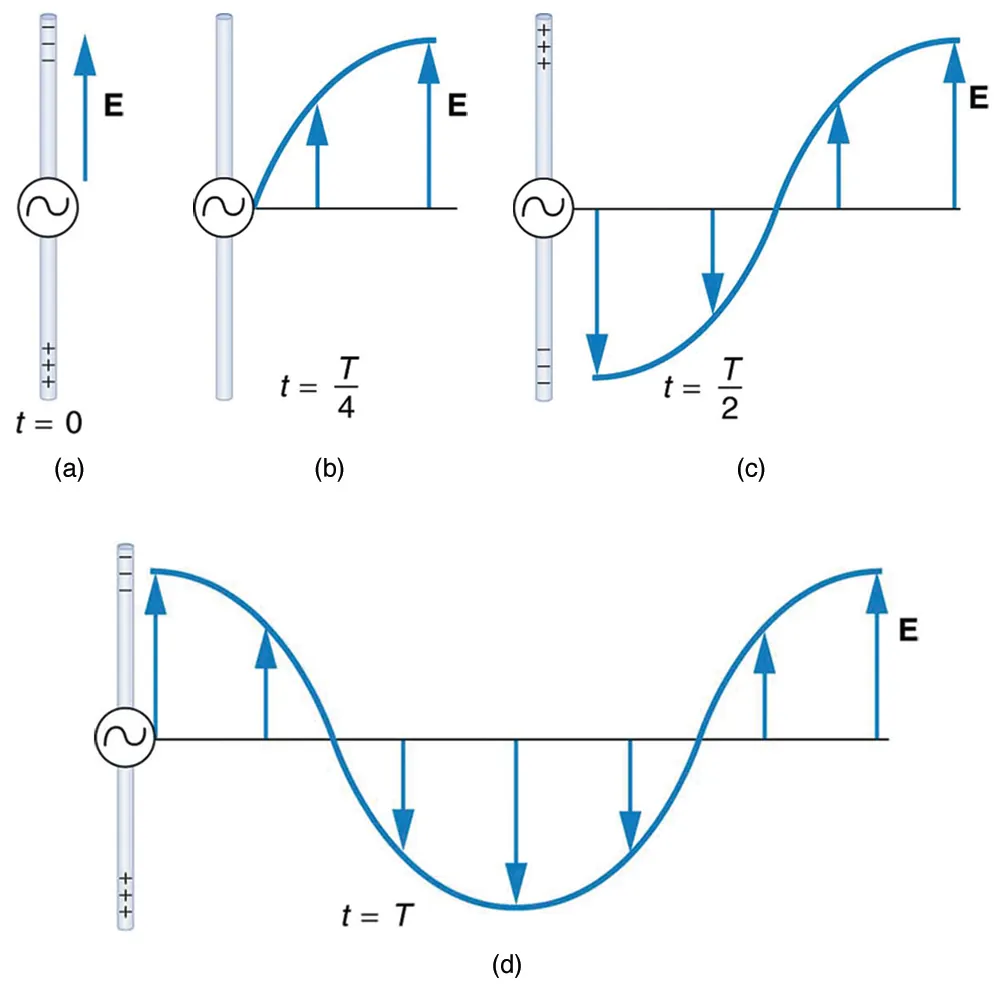
\includegraphics[width=0.55\textwidth]{figures/gen1.png}
%\caption{\label{fig:gen1} An AC voltage source corresponds to electrons oscilatting, which leads to an oscilatting field.}
%\end{figure}
%\end{frame}
%
%\begin{frame}{Electromagnetic waves: Electromagnetic wave production}
%\begin{figure}
%\centering
%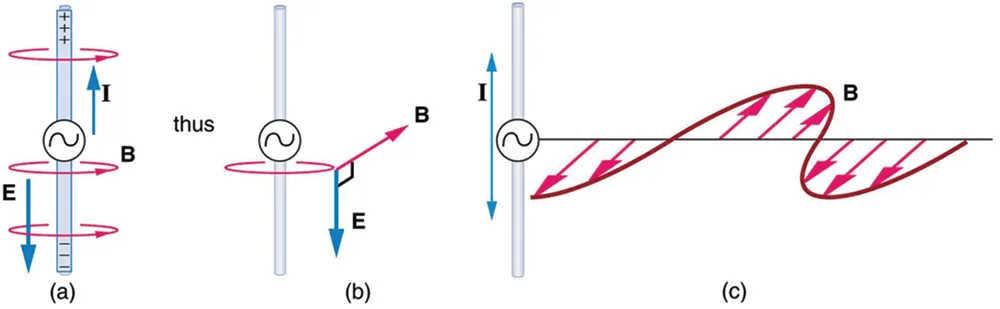
\includegraphics[width=0.9\textwidth]{figures/gen2.png}
%\caption{\label{fig:gen2} The oscillating E-field generates an orthogonal B-field.}
%\end{figure}
%\end{frame}
%
%\begin{frame}{Electromagnetic waves: Electromagnetic wave production}
%\begin{figure}
%\centering
%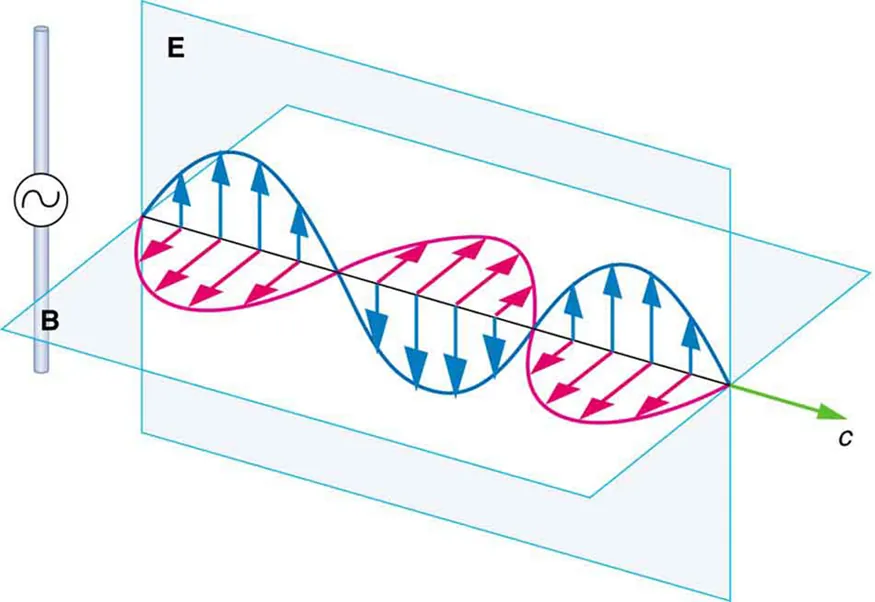
\includegraphics[width=0.75\textwidth]{figures/gen3.png}
%\caption{\label{fig:gen3} The oscillating B-field generates an orthogonal E-field, continuing the process.}
%\end{figure}
%\end{frame}
%
%\begin{frame}{Electromagnetic waves: Electromagnetic wave production}
%The wave \textbf{\alert{moves energy}} in the direction of the green arrow.
%\begin{figure}
%\centering
%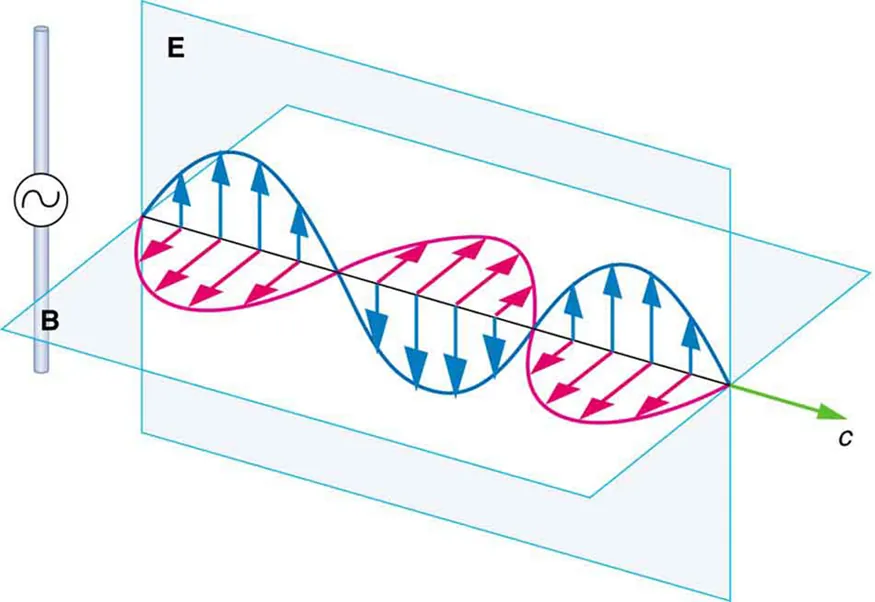
\includegraphics[width=0.35\textwidth]{figures/gen3.png}
%\caption{\label{fig:gen4} The oscillating B-field generates an orthogonal E-field, continuing the process.}
%\end{figure}
%The flux of energy per unit area in this case is (after some length mathematics)
%\begin{equation}
%\vec{S} = \frac{1}{\mu_0} \vec{E} \times \vec{B}
%\end{equation}
%\end{frame}
%
%\begin{frame}{Electromagnetic waves: Electromagnetic wave production}
%The wave \textbf{\alert{moves energy}} in the direction of $\vec{S}$.  The direction is orthogonal to the E and B, with a magnitude $EB/\mu_0$.  The peak B-value is $B = E/c$.  Both B and E are sinusoids with the same $f$ and $\phi$.  Thus, $S \propto \sin^2(2\pi ft +\phi)$, and the average of this is $1/2$.  This makes the average \textbf{\alert{intensity}}
%\begin{equation}
%\bar{S} = \frac{1}{2c\mu_0}E^2
%\end{equation}
%The units of intensity are W m$^{-2}$.  This formula is useful:
%\begin{itemize}
%\item Calculate the RX power at a radio given the field strength at the radio station, and the distance to the radio station.
%\item Calculate the brightness of a star observed at Earth, given the field strength of the light at the star.
%\end{itemize}
%\end{frame}
%
%\begin{frame}{Electromagnetic waves: Electromagnetic wave production}
%Suppose a microwave in the kitchen generates 1 kW of power, projected onto a 10cm x 10cm area at a distance of 1 m.  What is the intensity (power per unit area)?
%\begin{itemize}
%\item C: 1 kW
%\item D: 100 kW
%\item A: 1 kW m$^{-2}$
%\item B: 100 kW m$^{-2}$
%\end{itemize}
%\end{frame}
%
%\begin{frame}{Electromagnetic waves: Electromagnetic wave production}
%Suppose a microwave in the kitchen generates 1 kW of power, projected onto a 10cm x 10cm area at a distance of 1 m.  How long does it take the energy to travel the 1 meter?
%\begin{itemize}
%\item C: 0.333 ns
%\item D: 3.33 ns
%\item A: 33.3 ns
%\item B: 333 ns
%\end{itemize}
%\end{frame}
%
%\begin{frame}{Electromagnetic waves: Electromagnetic wave production}
%Suppose a microwave in the kitchen generates 1 kW of power, projected onto a 10cm x 10cm area at a distance of 1 m.  What is the peak E-field at the source?
%\begin{itemize}
%\item C: 870 V/m
%\item D: 8700 V
%\item A: 8700 V/m
%\item B: 870 V
%\end{itemize}
%\end{frame}
%
%\section{Electromagnetic waves: Electromagnetic spectrum and energy}
%
%\begin{frame}{Electromagnetic waves: Electromagnetic spectrum and energy}
%\small
%\begin{figure}
%\centering
%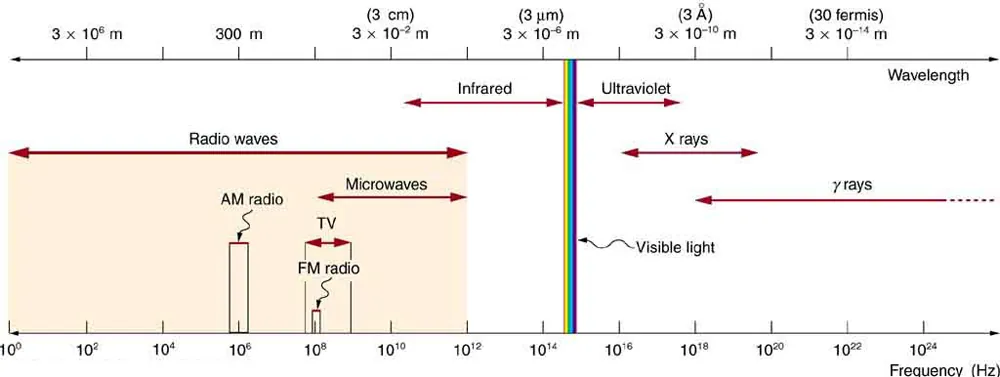
\includegraphics[width=0.95\textwidth]{figures/spectrum.png}
%\caption{\label{fig:spectrum} \textbf{\alert{The electromagnetic spectrum}} maps signal types to wavelength (top) and frequency (bottom).}
%\end{figure}
%\begin{itemize}
%\item Visible spectrum: more than $10^{14}$ Hz, 400-700 nm wavelengths
%\item Radio waves: $[10^{-1} - 10^4]$ MHz
%\end{itemize}
%\end{frame}
%
%\begin{frame}{Electromagnetic waves: Electromagnetic spectrum and energy}
%\small
%\textbf{\alert{Amplitude modulation (AM)}} is a technology that allows audio transmission over the EM spectrum.
%\begin{figure}
%\centering
%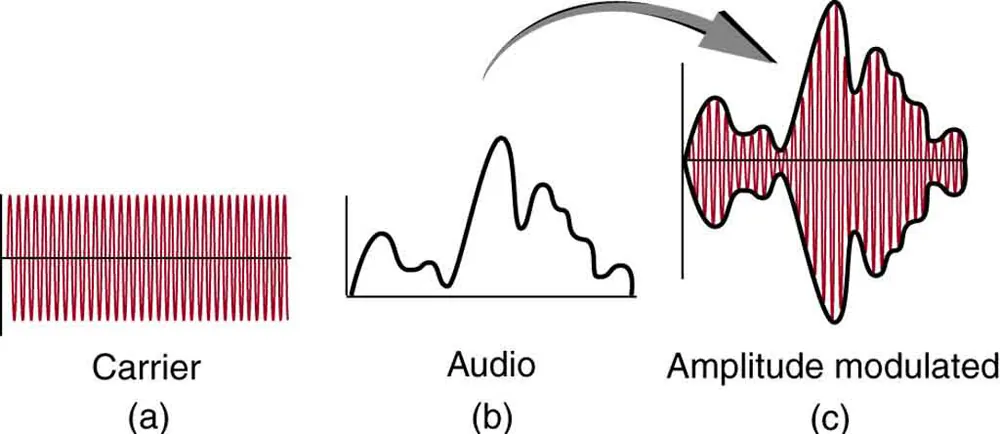
\includegraphics[width=0.85\textwidth]{figures/AM.png}
%\caption{\label{fig:radio} (a) The carrier wave. (b) The audio spectrum. (c) The \textit{modulated} carrier wave.}
%\end{figure}
%\end{frame}
%
%\begin{frame}{Electromagnetic waves: Electromagnetic spectrum and energy}
%\footnotesize
%\begin{columns}[T]
%\begin{column}{0.5\textwidth}
%The carrier is a pure sinusoid at a single frequency, $f_{\rm c}$, with amplitude $A$:
%\begin{equation}
%c(t) = A\sin(2\pi f_{\rm c} t) \label{eq:carrier}
%\end{equation}
%Let the modulating audio signal (at a given frequency) be
%\begin{equation}
%m(t) = Am\cos(2\pi f_{\rm m} t + \phi) \label{eq:modulation}
%\end{equation}
%Audio waves are not electromagnetic, and audio frequencies are orders of magnitude smaller than radio frequencies.  If there were a way to \textit{mix} (multiply) these signals \textbf{\alert{as voltages}}, then we get
%\begin{equation}
%y(t) = \left[1+\frac{m(t)}{A}\right]c(t) \label{eq:mix}
%\end{equation}
%\end{column}
%\begin{column}{0.5\textwidth}
%Do you remember the following trigonometric identity?
%\begin{multline}
%\sin(A)\cos(B) = \\ \frac{1}{2}\left(\sin(A+B) + \sin(A-B)\right) \label{eq:ident}
%\end{multline}
%\textbf{Group exercise:}
%Substitute Eqs. \ref{eq:carrier} and \ref{eq:modulation} into \ref{eq:mix}, and use the trigonometric identity in Eq. \ref{eq:ident} to simplify the result.
%\begin{enumerate}
%\item Look for three waves: the carrier, and two additional ones at two different frequencies.
%\item Draw a picture of the spectrum, the amplitude versus frequency of the signal.
%\end{enumerate}
%\end{column}
%\end{columns}
%\end{frame}
%
%\begin{frame}{Electromagnetic waves: Electromagnetic spectrum and energy}
%\footnotesize
%\begin{columns}[T]
%\begin{column}{0.5\textwidth}
%The AM mixing yields three waves:
%\begin{itemize}
%\item The original carrier
%\item A wave with $f_{\rm c} + f_{\rm m}$
%\item A wave with $f_{\rm c} - f_{\rm m}$
%\end{itemize}
%To re-capture the audio, we must \textit{demodulate}, or reverse the process.  \\ \vspace{0.5cm}\textbf{How do we create} $m(t)$, and how do we modulate and demodulate it?
%\begin{itemize}
%\item Parallel LC circuits that act as resonators
%\item Diodes, devices that allow current to flow only one way
%\end{itemize}
%\end{column}
%\begin{column}{0.5\textwidth}
%\begin{figure}
%\centering
%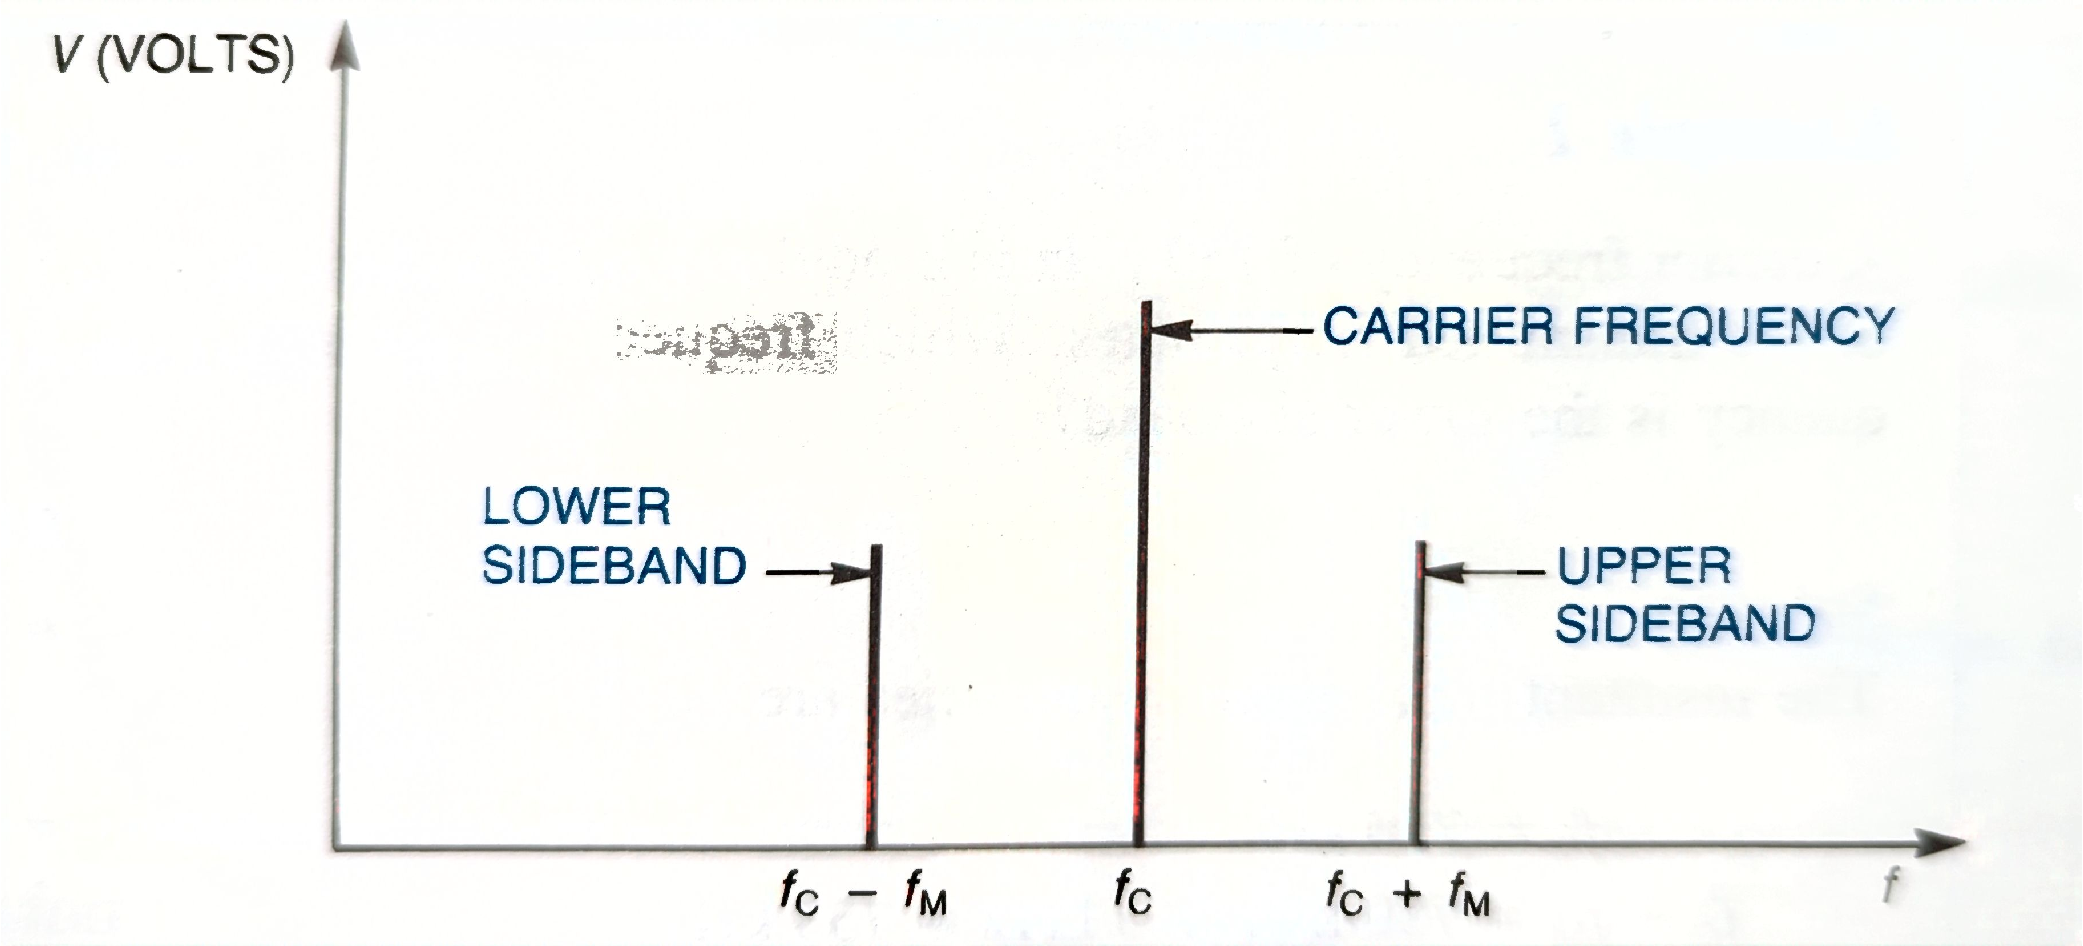
\includegraphics[width=0.95\textwidth]{figures/AMSpec.pdf}
%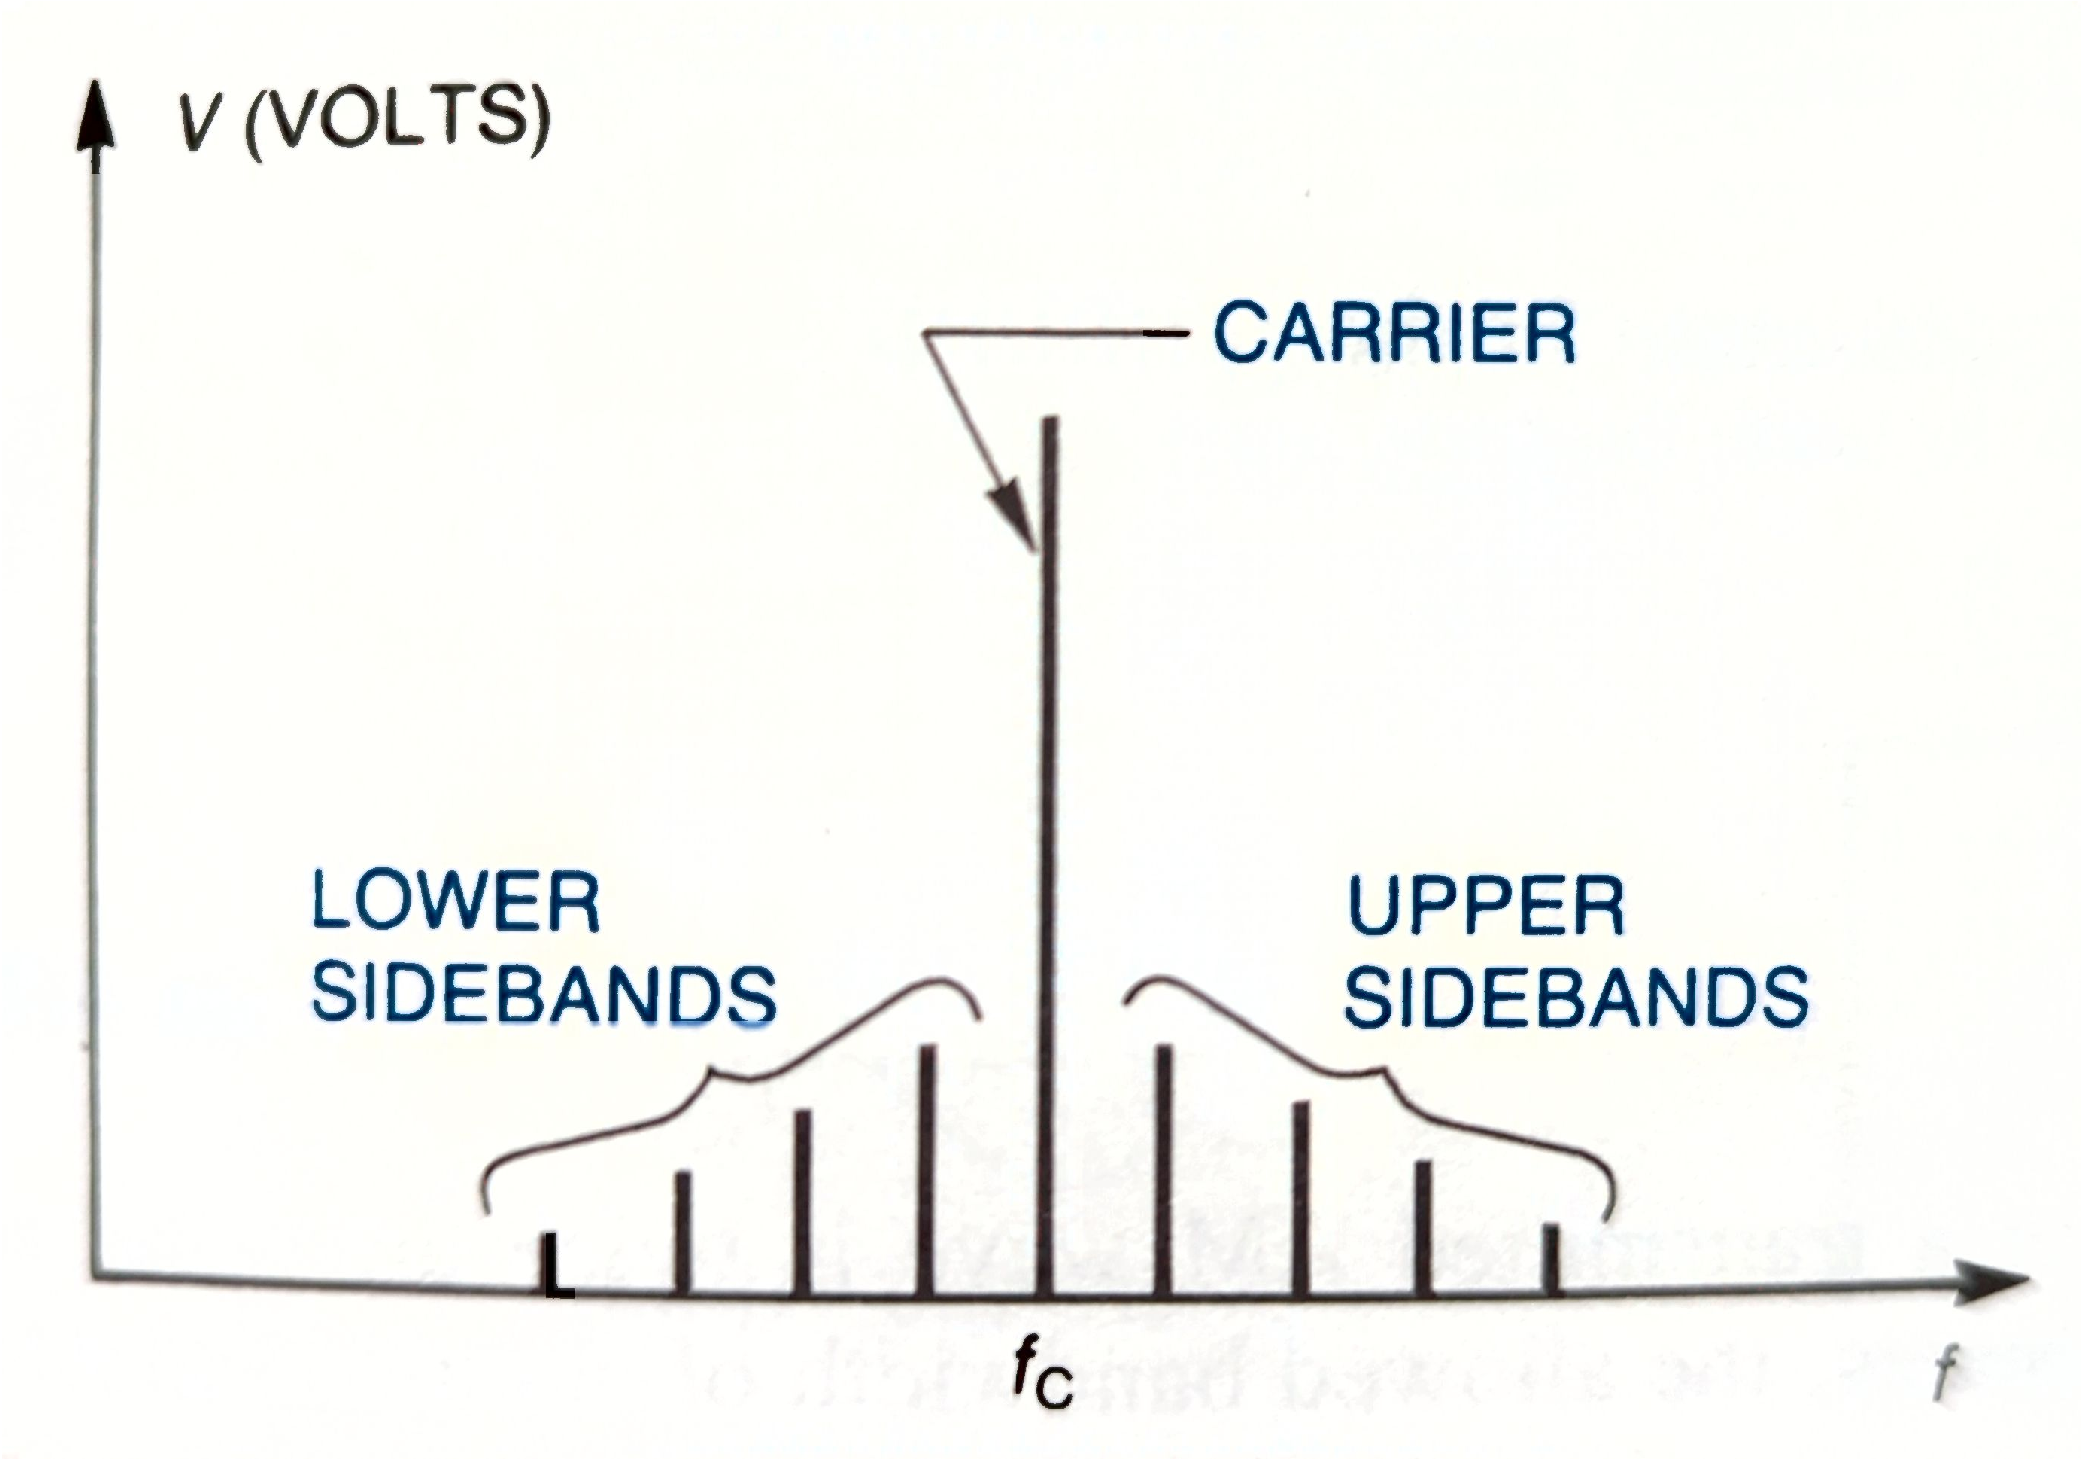
\includegraphics[width=0.75\textwidth]{figures/AMSpec2.pdf}
%\caption{\label{fig:amspec} \footnotesize (Top) An example of a single audio frequency mixed into an AM signal. (Bottom) An audio spectrum mixed into an AM signal.}
%\end{figure}
%\end{column}
%\end{columns}
%\end{frame}
%
%\begin{frame}{Electromagnetic waves: Electromagnetic spectrum and energy}
%\footnotesize
%\begin{columns}[T]
%\begin{column}{0.35\textwidth}
%\textbf{How do we create} $m(t)$, and how do we modulate and demodulate it?
%\begin{itemize}
%\item Parallel LC circuits that act as resonators
%\item Diodes, devices that allow current to flow only one way
%\end{itemize}
%\begin{figure}
%\centering
%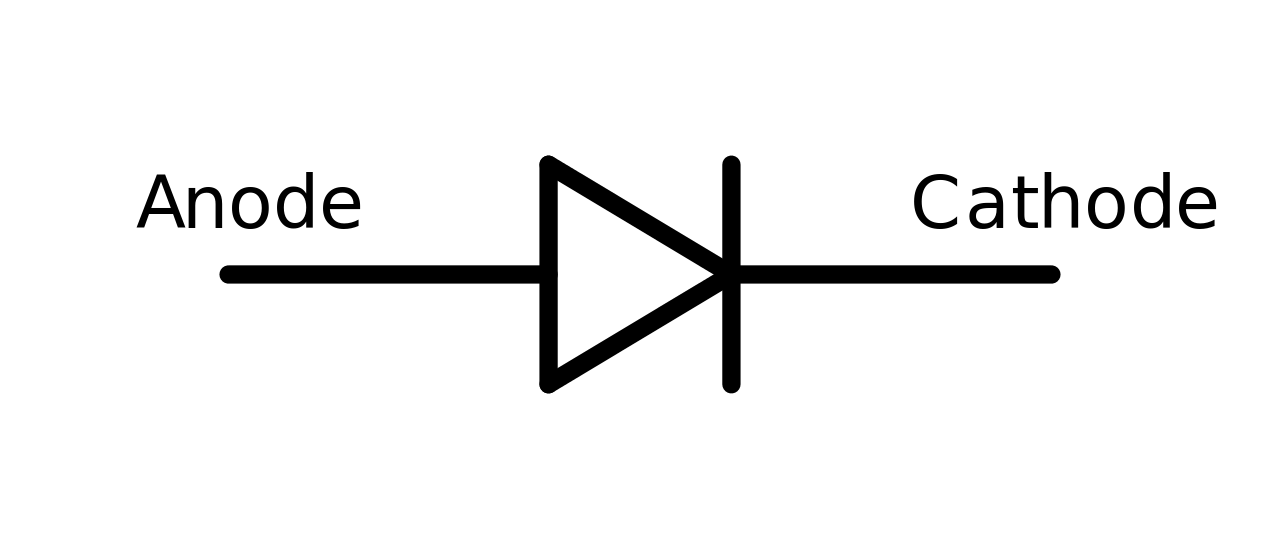
\includegraphics[width=0.95\textwidth]{figures/diode.png}
%\caption{\label{fig:diode} \footnotesize Circuit diagram for the diode.}
%\end{figure}
%\end{column}
%\begin{column}{0.65\textwidth}
%\begin{figure}
%\centering
%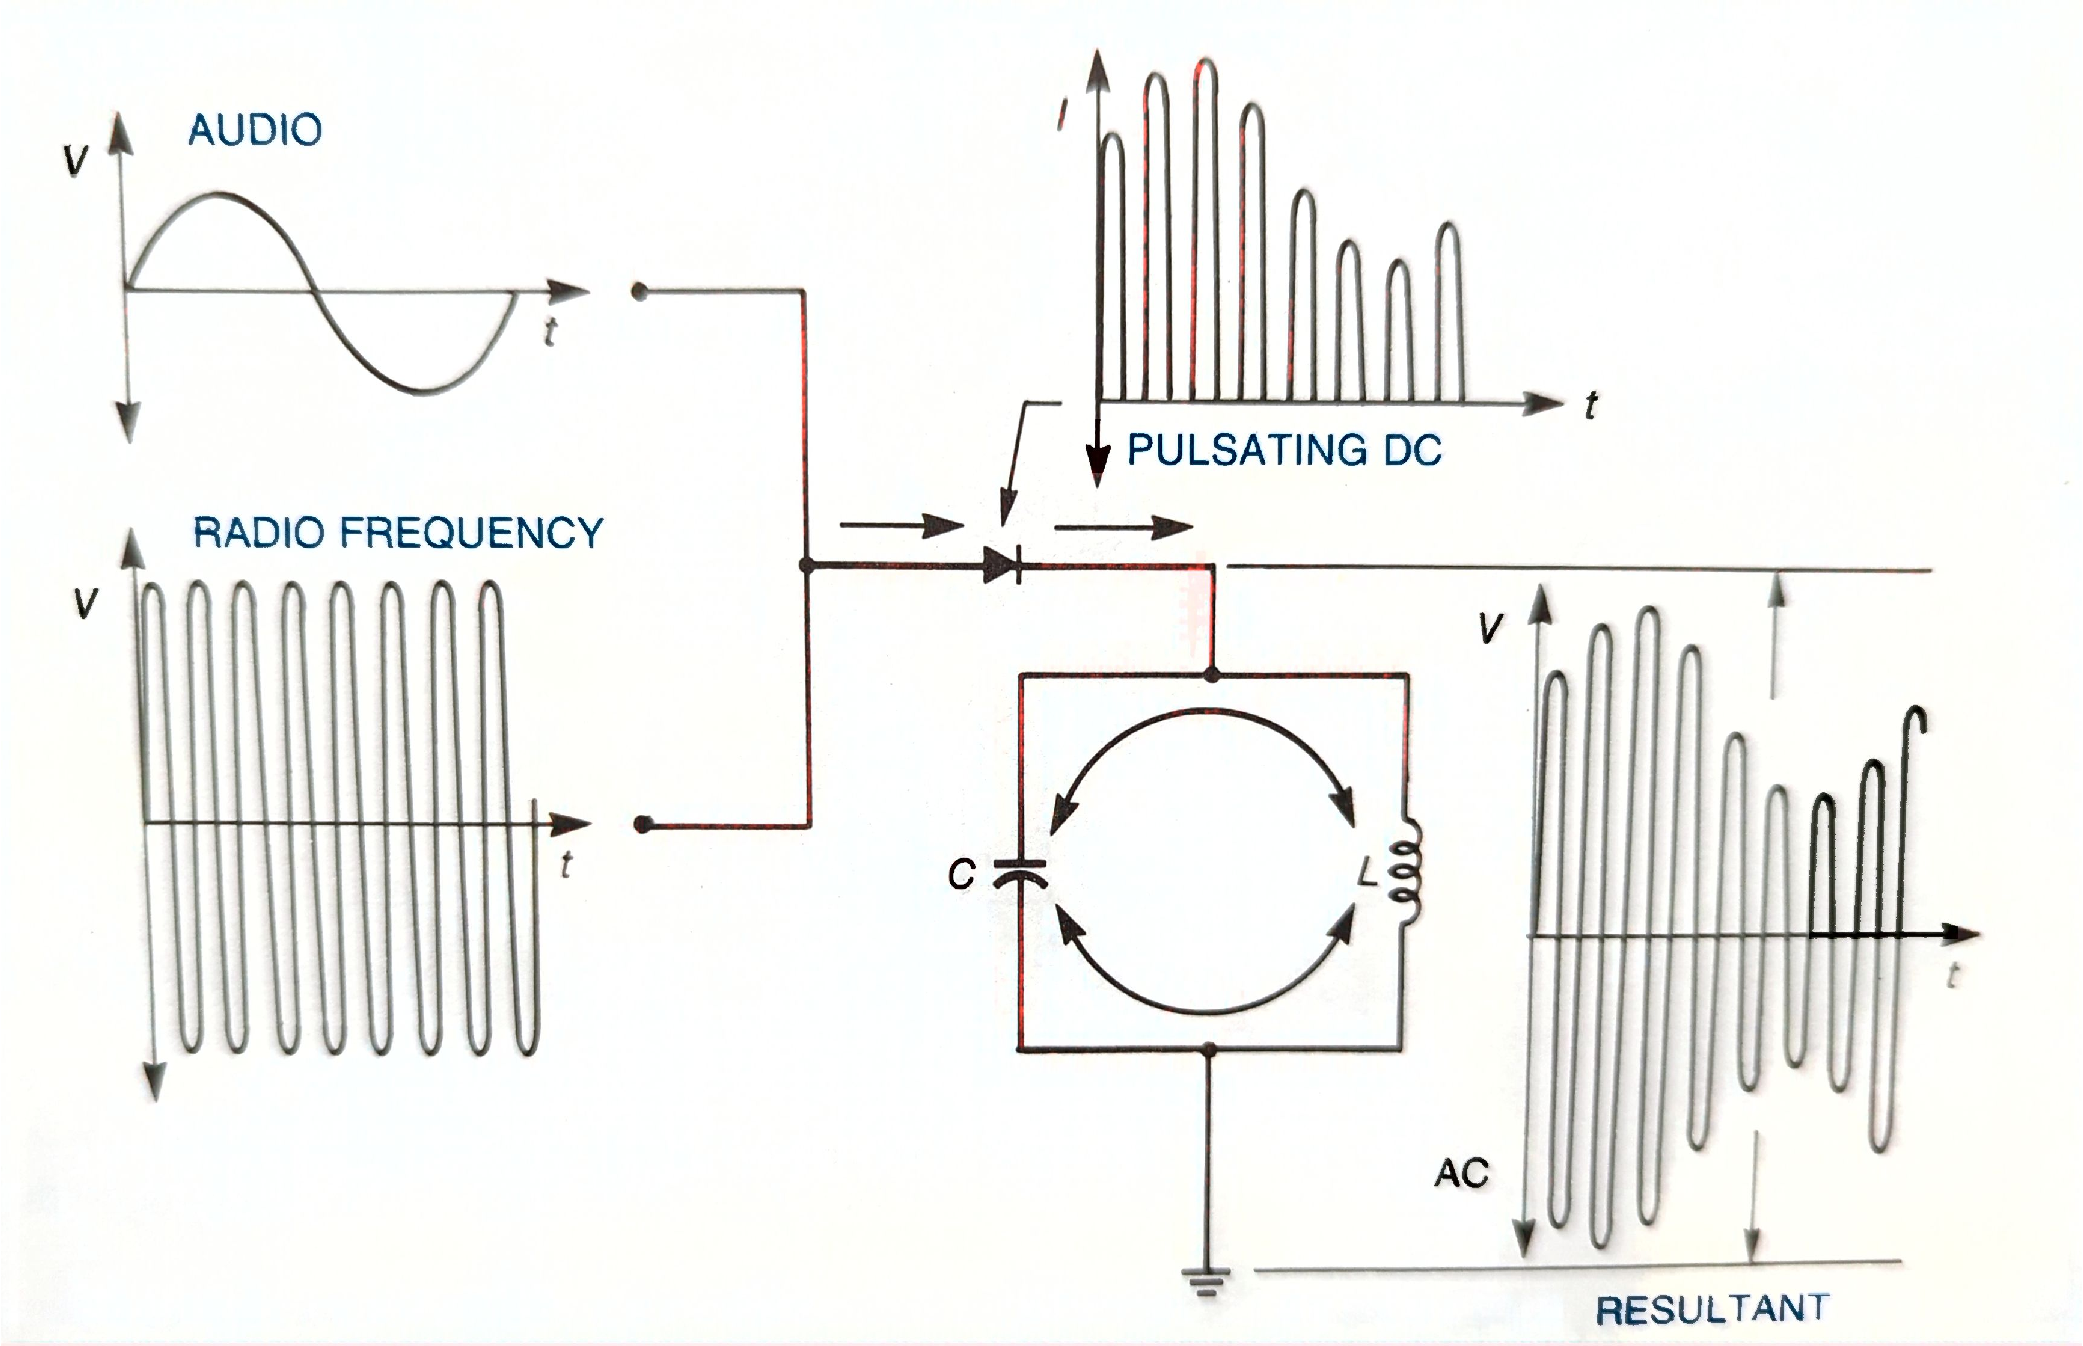
\includegraphics[width=0.95\textwidth]{figures/AMSpec3.pdf}
%\caption{\label{fig:amspec2} \footnotesize (Upper left) The audio signal is converted to a voltage via a microphone. (Lower left) The radio carrier signal oscillates at a higher frequency. (Middle) The LC resonator and diode mix the two signals. (Right) The final amplitude is modulated by the audio.}
%\end{figure}
%\end{column}
%\end{columns}
%\end{frame}
%
%\begin{frame}{Electromagnetic waves: Electromagnetic spectrum and energy}
%Suppose an audio signal exists primarily at 10 kHz, and we need an AM carrier at 1.4 MHz.  If this AM carrier is mixed with the audio signal, what frequencies will exist in the final signal?
%\begin{itemize}
%\item A: 1390 and 1400 kHz
%\item B: 1400 kHz only
%\item C: 1390, 1400, and 1410 kHz
%\item D: 1390 and 1410 kHz
%\end{itemize}
%\end{frame}
%
%\begin{frame}{Electromagnetic waves: Electromagnetic spectrum and energy}
%Suppose an audio signal exists primarily at 10 kHz, and we need an AM carrier at 1.4 MHz.  If this AM carrier is mixed with the audio signal, what is the \textit{bandwidth} required?  That is, how much of the EM spectrum is occupied by the final signal?
%\begin{itemize}
%\item A: 10 kHz
%\item B: 20 kHz
%\item C: 1400 kHz
%\item D: 1420 kHz
%\end{itemize}
%\end{frame}
%
%\begin{frame}{Electromagnetic waves: Electromagnetic spectrum and energy}
%Suppose an audio signal exists primarily at 10 kHz, and we need an AM carrier at 1.4 MHz.  If, in our mixer, $L = 10$ $\mu$H is required, what value must we choose for $C$?
%\begin{itemize}
%\item A: 1.3 mF
%\item B: 2.6 $\mu$F
%\item C: 1.3 $\mu$F
%\item D: 1.3 nF
%\end{itemize}
%\end{frame}
%
%\begin{frame}{Electromagnetic waves: Electromagnetic spectrum and energy}
%\begin{figure}
%\centering
%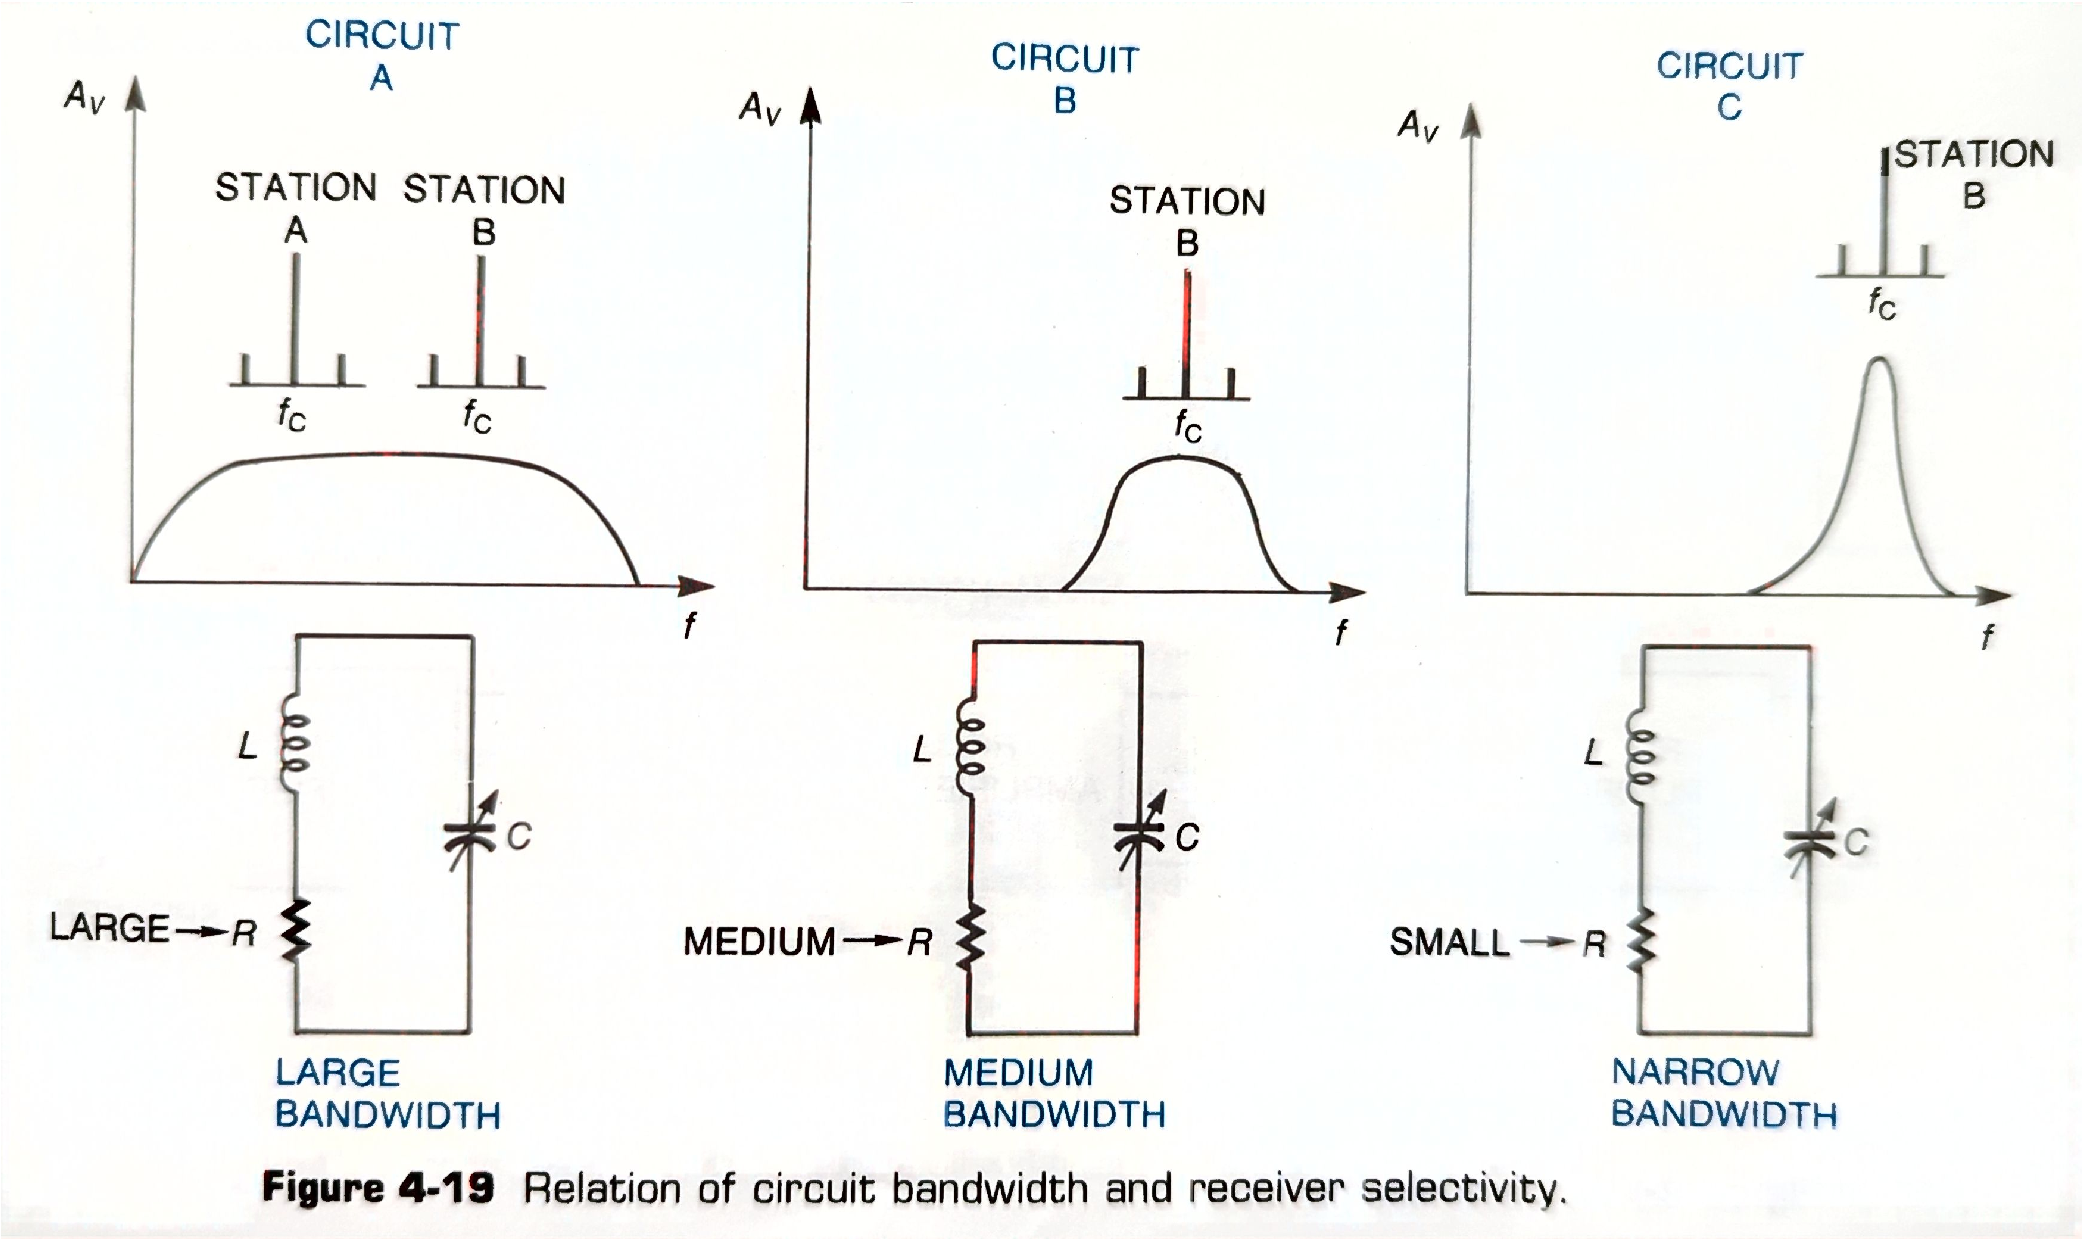
\includegraphics[width=0.65\textwidth]{figures/RX.pdf}
%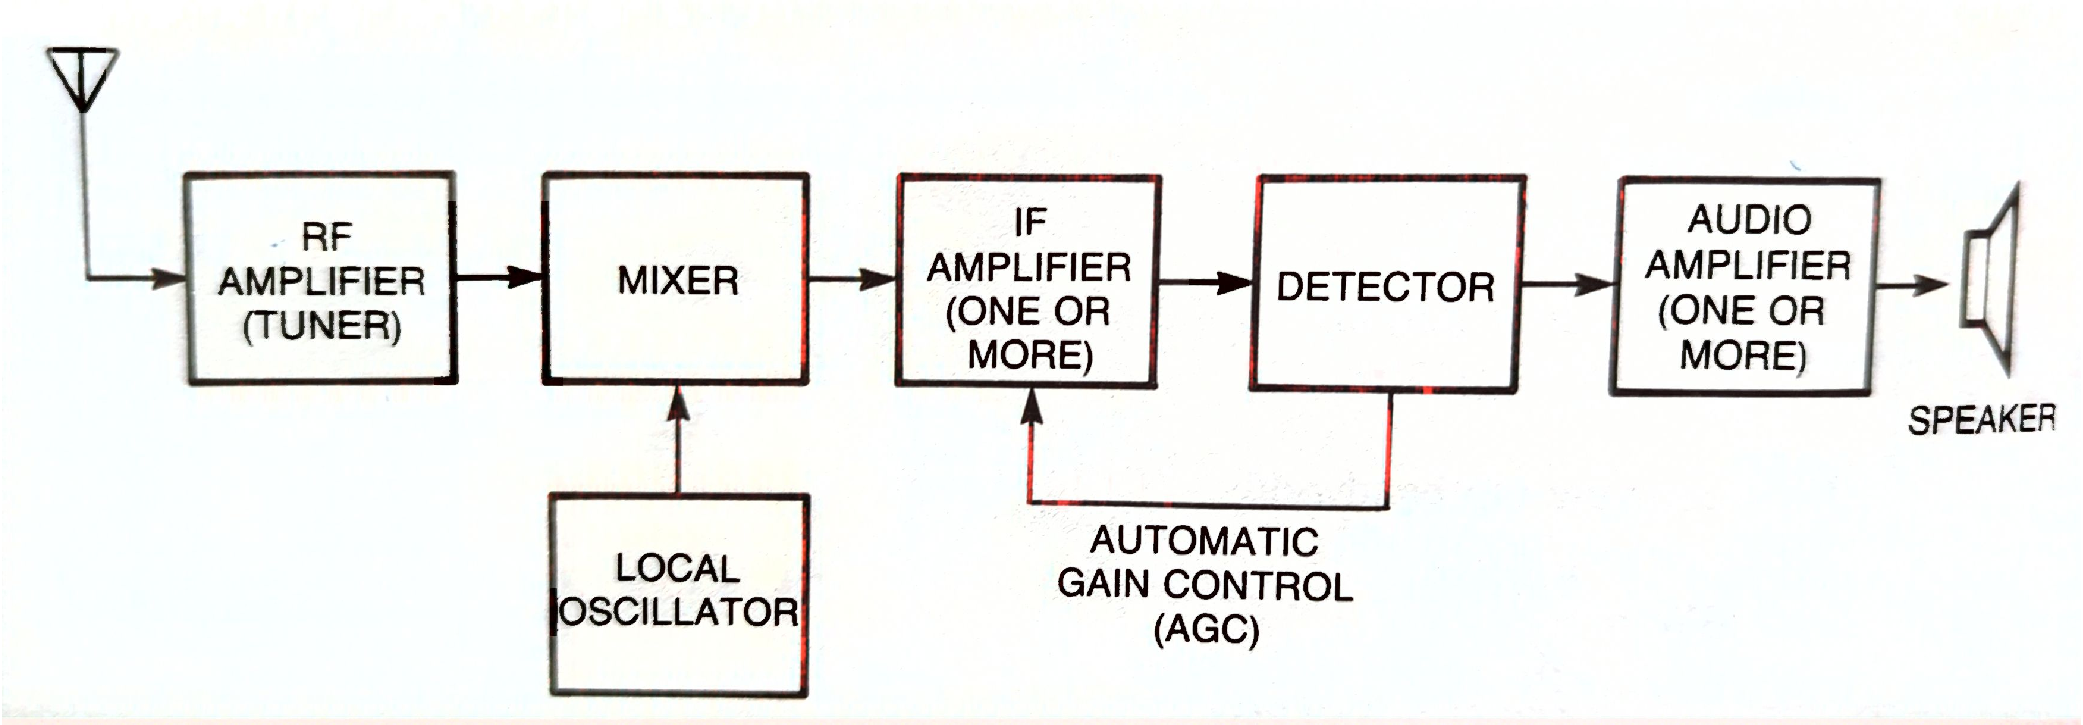
\includegraphics[width=0.65\textwidth]{figures/SuperHet.pdf}
%\caption{\label{fig:rx} \footnotesize Circuit properties for the AM receiver.}
%\end{figure}
%\end{frame}
%
%\begin{frame}{Electromagnetic waves: Electromagnetic spectrum and energy}
%We can show that the \textit{bandwidth} of the RLC response is
%\begin{equation}
%\frac{\Delta f}{f_0} = \omega_0 \tau = 2\pi f_0 \tau
%\end{equation}
%Where $\tau = RC$ and $f_0 = 1/(2\pi \sqrt{LC})$.  This simplifies to
%\begin{equation}
%\frac{\Delta f}{f_0} = R \sqrt{\frac{C}{L}}
%\end{equation}
%Thus, bandwidth is proportional to $R$, as shown in Fig. \ref{fig:rx}.
%\end{frame}
%
%\begin{frame}{Electromagnetic waves: Electromagnetic spectrum and energy}
%Suppose an audio signal exists primarily at 5 kHz, and we need an AM carrier at 1100 kHz.  This implies our sidebands will be at 1095 kHz and 1105 kHz, making our bandwidth 10 kHz centered around 1100 kHz.  If our resistance $R$ is such that we are capturing the carrier, but not the sidebands, we should:
%\begin{itemize}
%\item A: Decrease $R$
%\item B: Increase $R$
%\item C: Leave $R$ unchanged 
%\item D: Set $R$ to 0 Ohms
%\end{itemize}
%\end{frame}
%
%\begin{frame}{Electromagnetic waves: Electromagnetic spectrum and energy}
%\footnotesize
%\begin{columns}[T]
%\begin{column}{0.4\textwidth}
%The local oscillator (LO) is a tunable oscillator set to be 455 kHz above the AM channel.  For example:
%\begin{itemize}
%\item AM channel: 1200 kHz
%\item LO: 1655 kHz
%\item Mixer: 1655 kHz + 1200 kHz, 1655 kHz, and 1655 - 1200 kHz
%\item 455 kHz is the \textit{intermediate frequency} (IF)
%\item IF amplifier: responds only to 1655 - 1200 = 455 kHz
%\end{itemize}
%\end{column}
%\begin{column}{0.6\textwidth}
%\begin{figure}
%\centering
%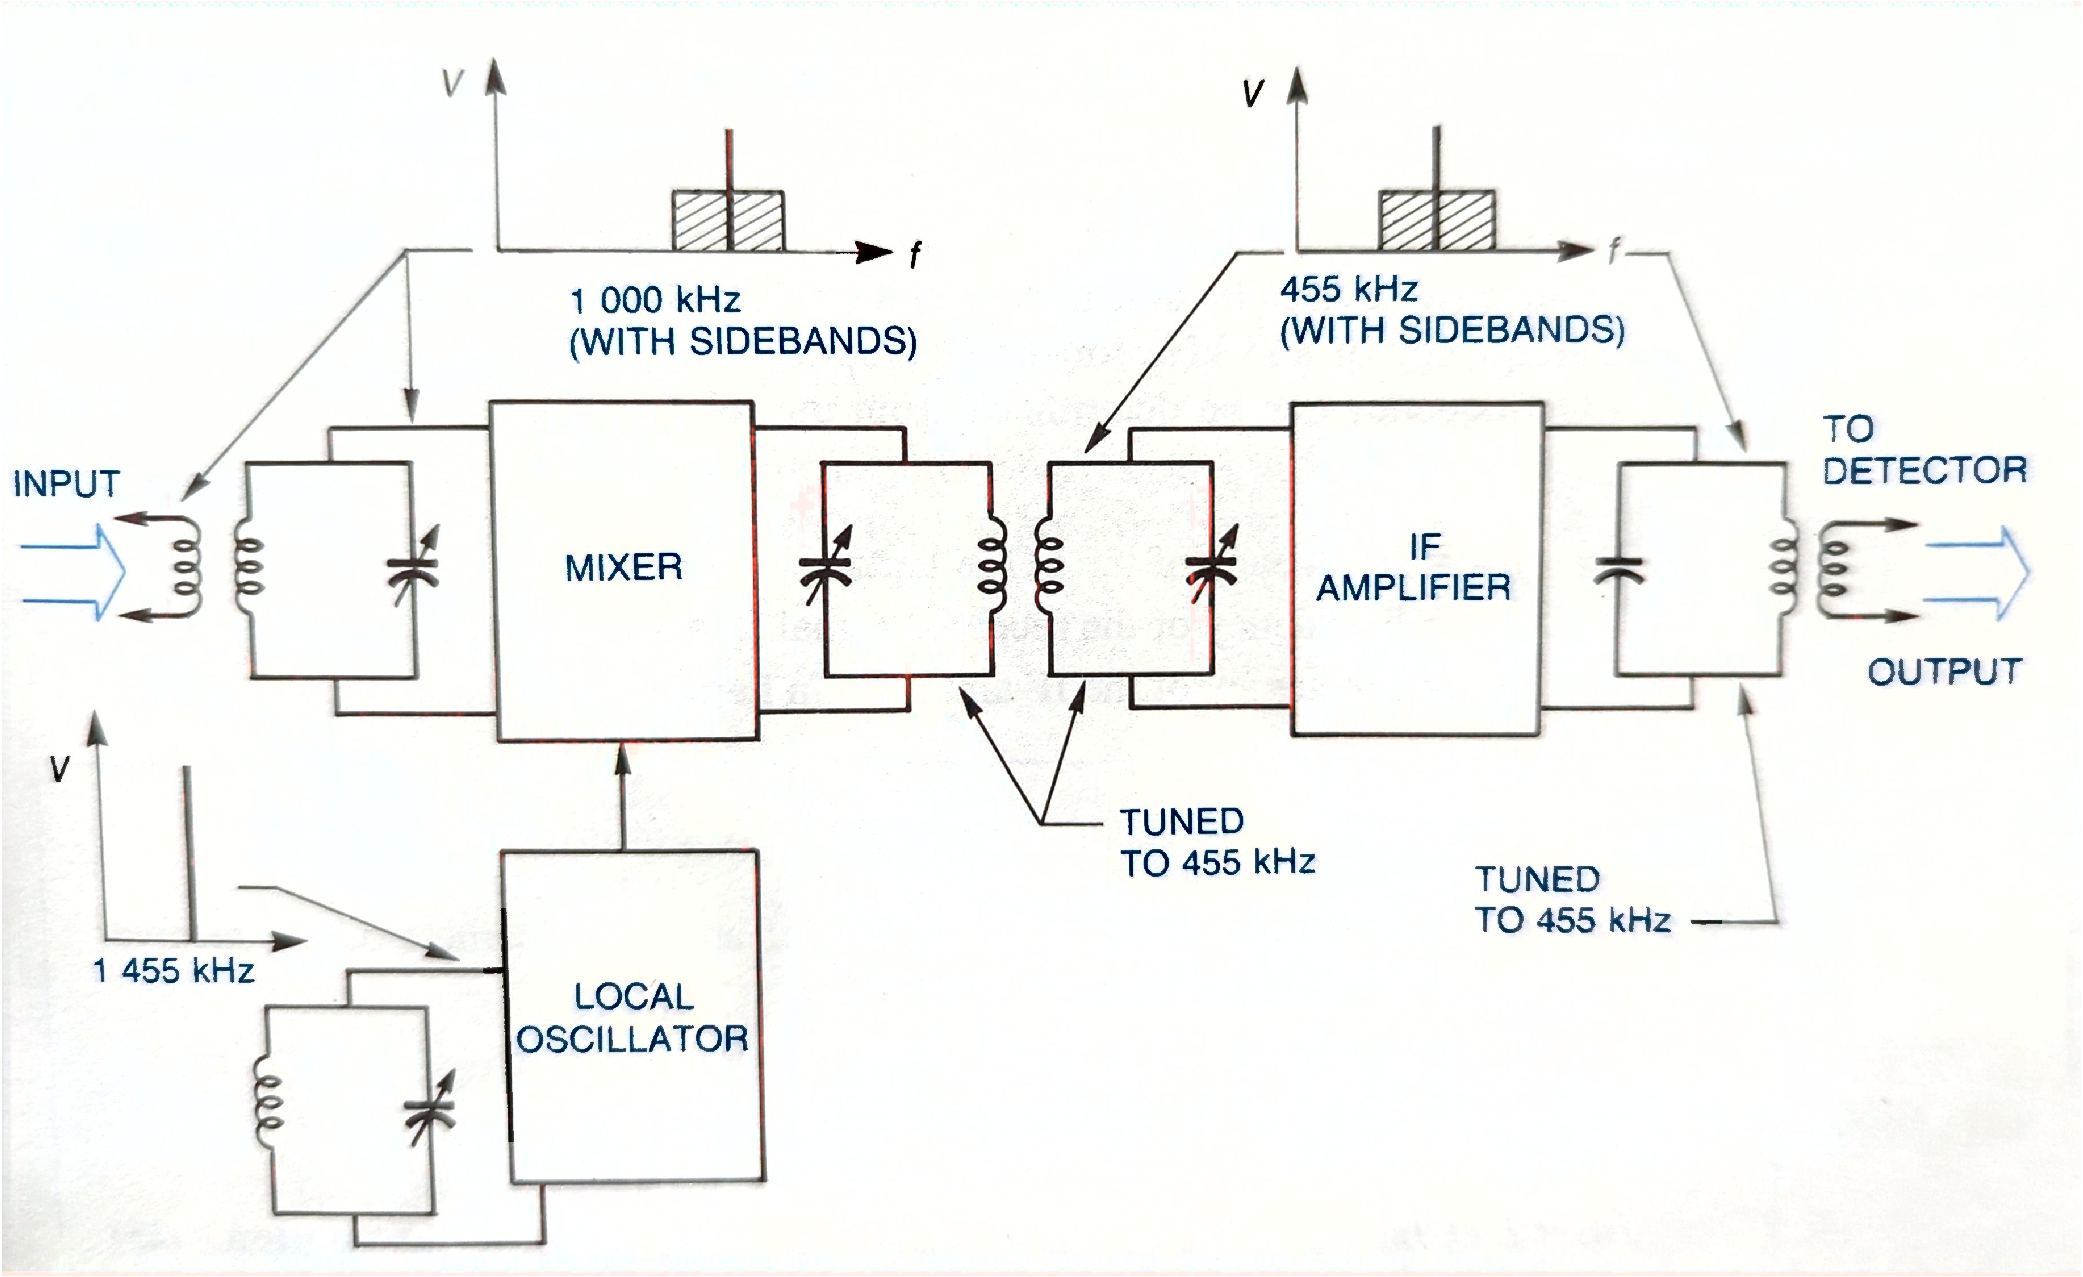
\includegraphics[width=\textwidth]{figures/SuperHet2.pdf}
%\caption{\label{fig:amspec3} \footnotesize The superheterodyne radio scheme.  Channel input is amplified, mixed with a local oscillator, and moved to the IF.  The IF is filtered and amplified, then demodulated in the detector.}
%\end{figure}
%\end{column}
%\end{columns}
%\end{frame}
%
%\begin{frame}{Electromagnetic waves: Electromagnetic spectrum and energy}
%Suppose an audio signal exists primarily at 10 kHz, and is mixed with a carrier at 1000 kHz.  What should our LO be if our IF is 455 kHz?
%\begin{itemize}
%\item A: 1000 kHz
%\item B: 455 kHz
%\item C: 545 kHz
%\item D: 1455 kHz
%\end{itemize}
%\end{frame}
%
%\begin{frame}{Electromagnetic waves: Electromagnetic spectrum and energy}
%\small
%\textbf{\alert{Frequency modulation}} (FM) radio transmission converts audio signals into frequency deviations in the carrier.
%\begin{figure}
%\centering
%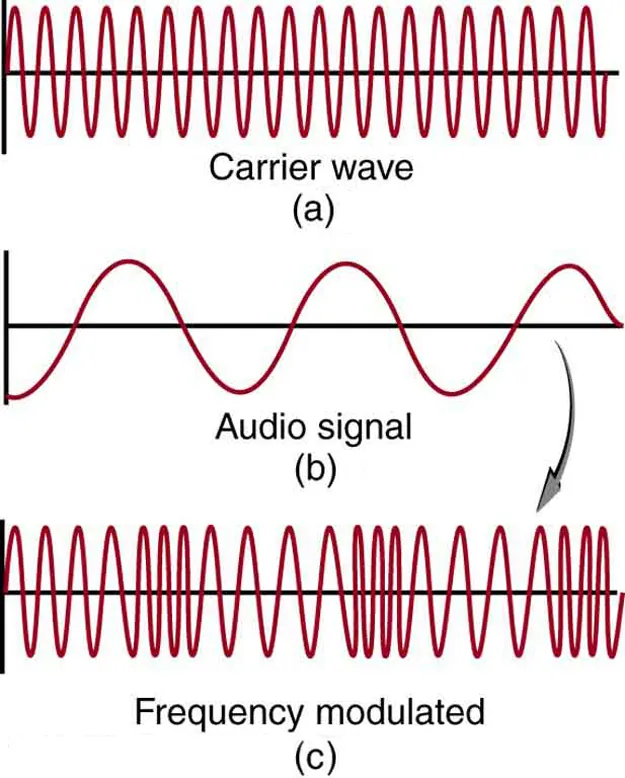
\includegraphics[width=0.35\textwidth]{figures/FM.png}
%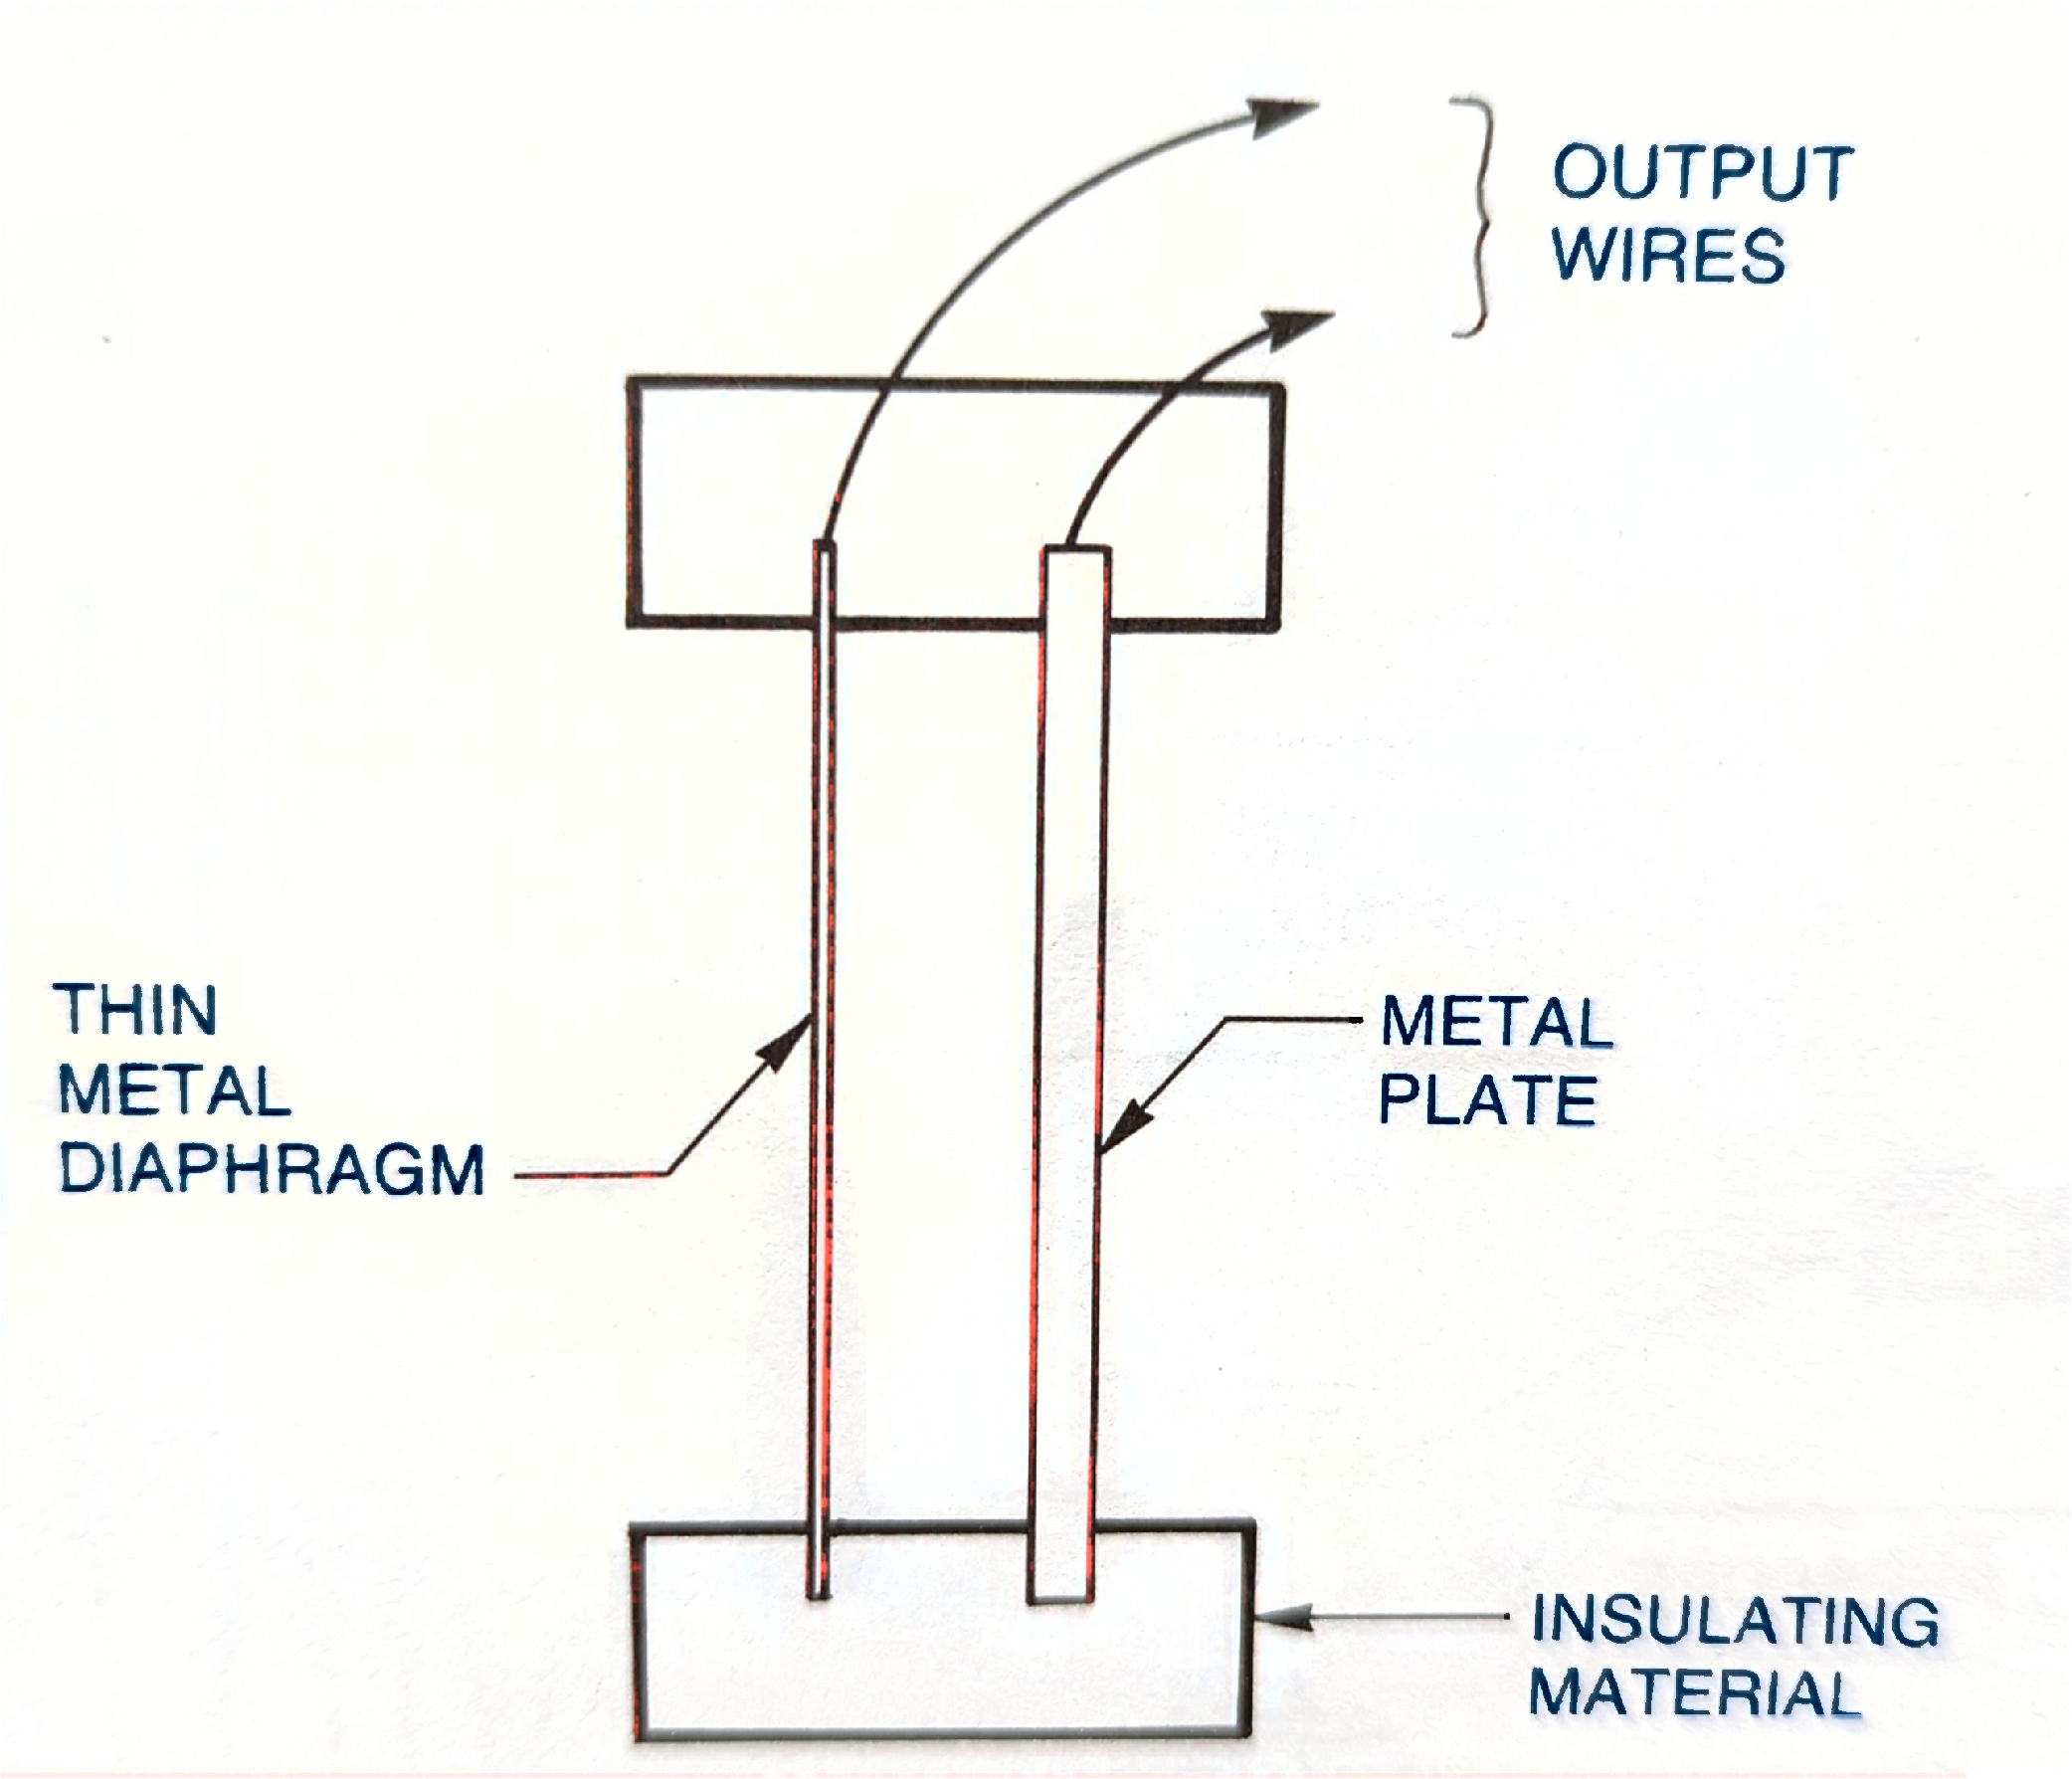
\includegraphics[width=0.55\textwidth]{figures/FMSpec.pdf}
%\caption{\label{fig:radio2} \footnotesize (Left) Frequency modulation. (Right) Capacitance microphone.}
%\end{figure}
%\end{frame}
%
%\begin{frame}{Electromagnetic waves: Electromagnetic spectrum and energy}
%\begin{figure}
%\centering
%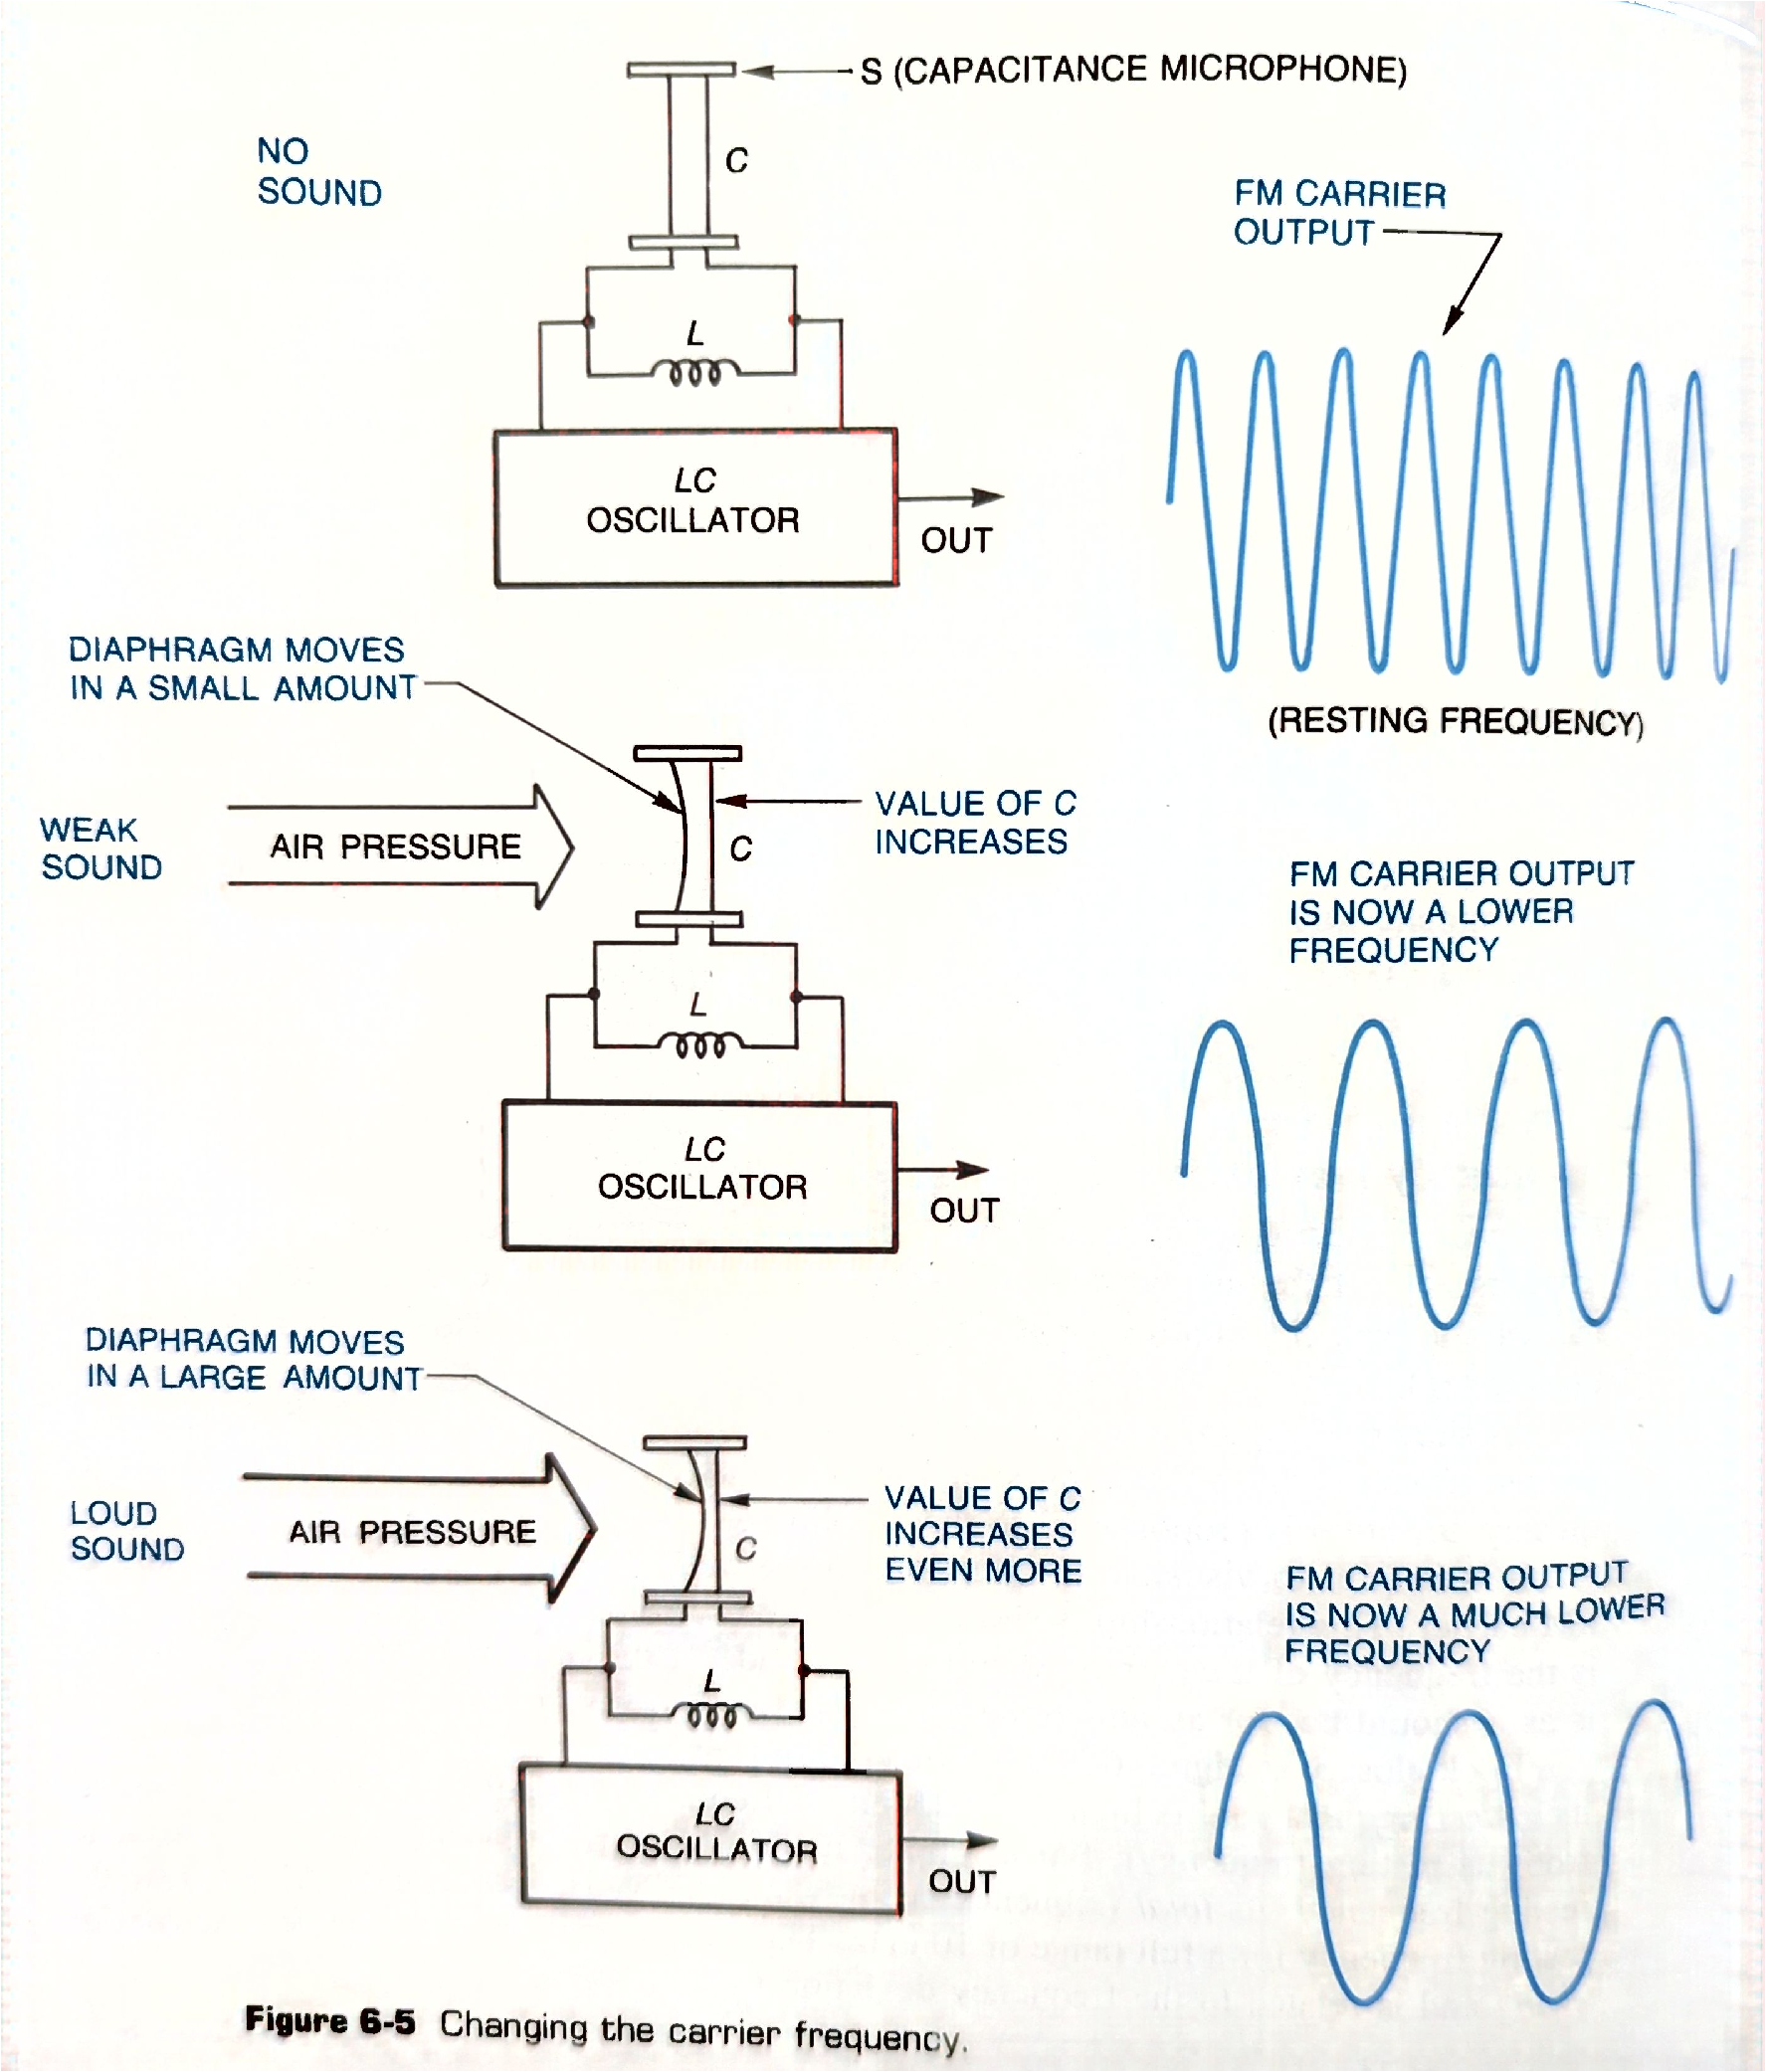
\includegraphics[width=0.475\textwidth]{figures/FMSpec2.pdf}
%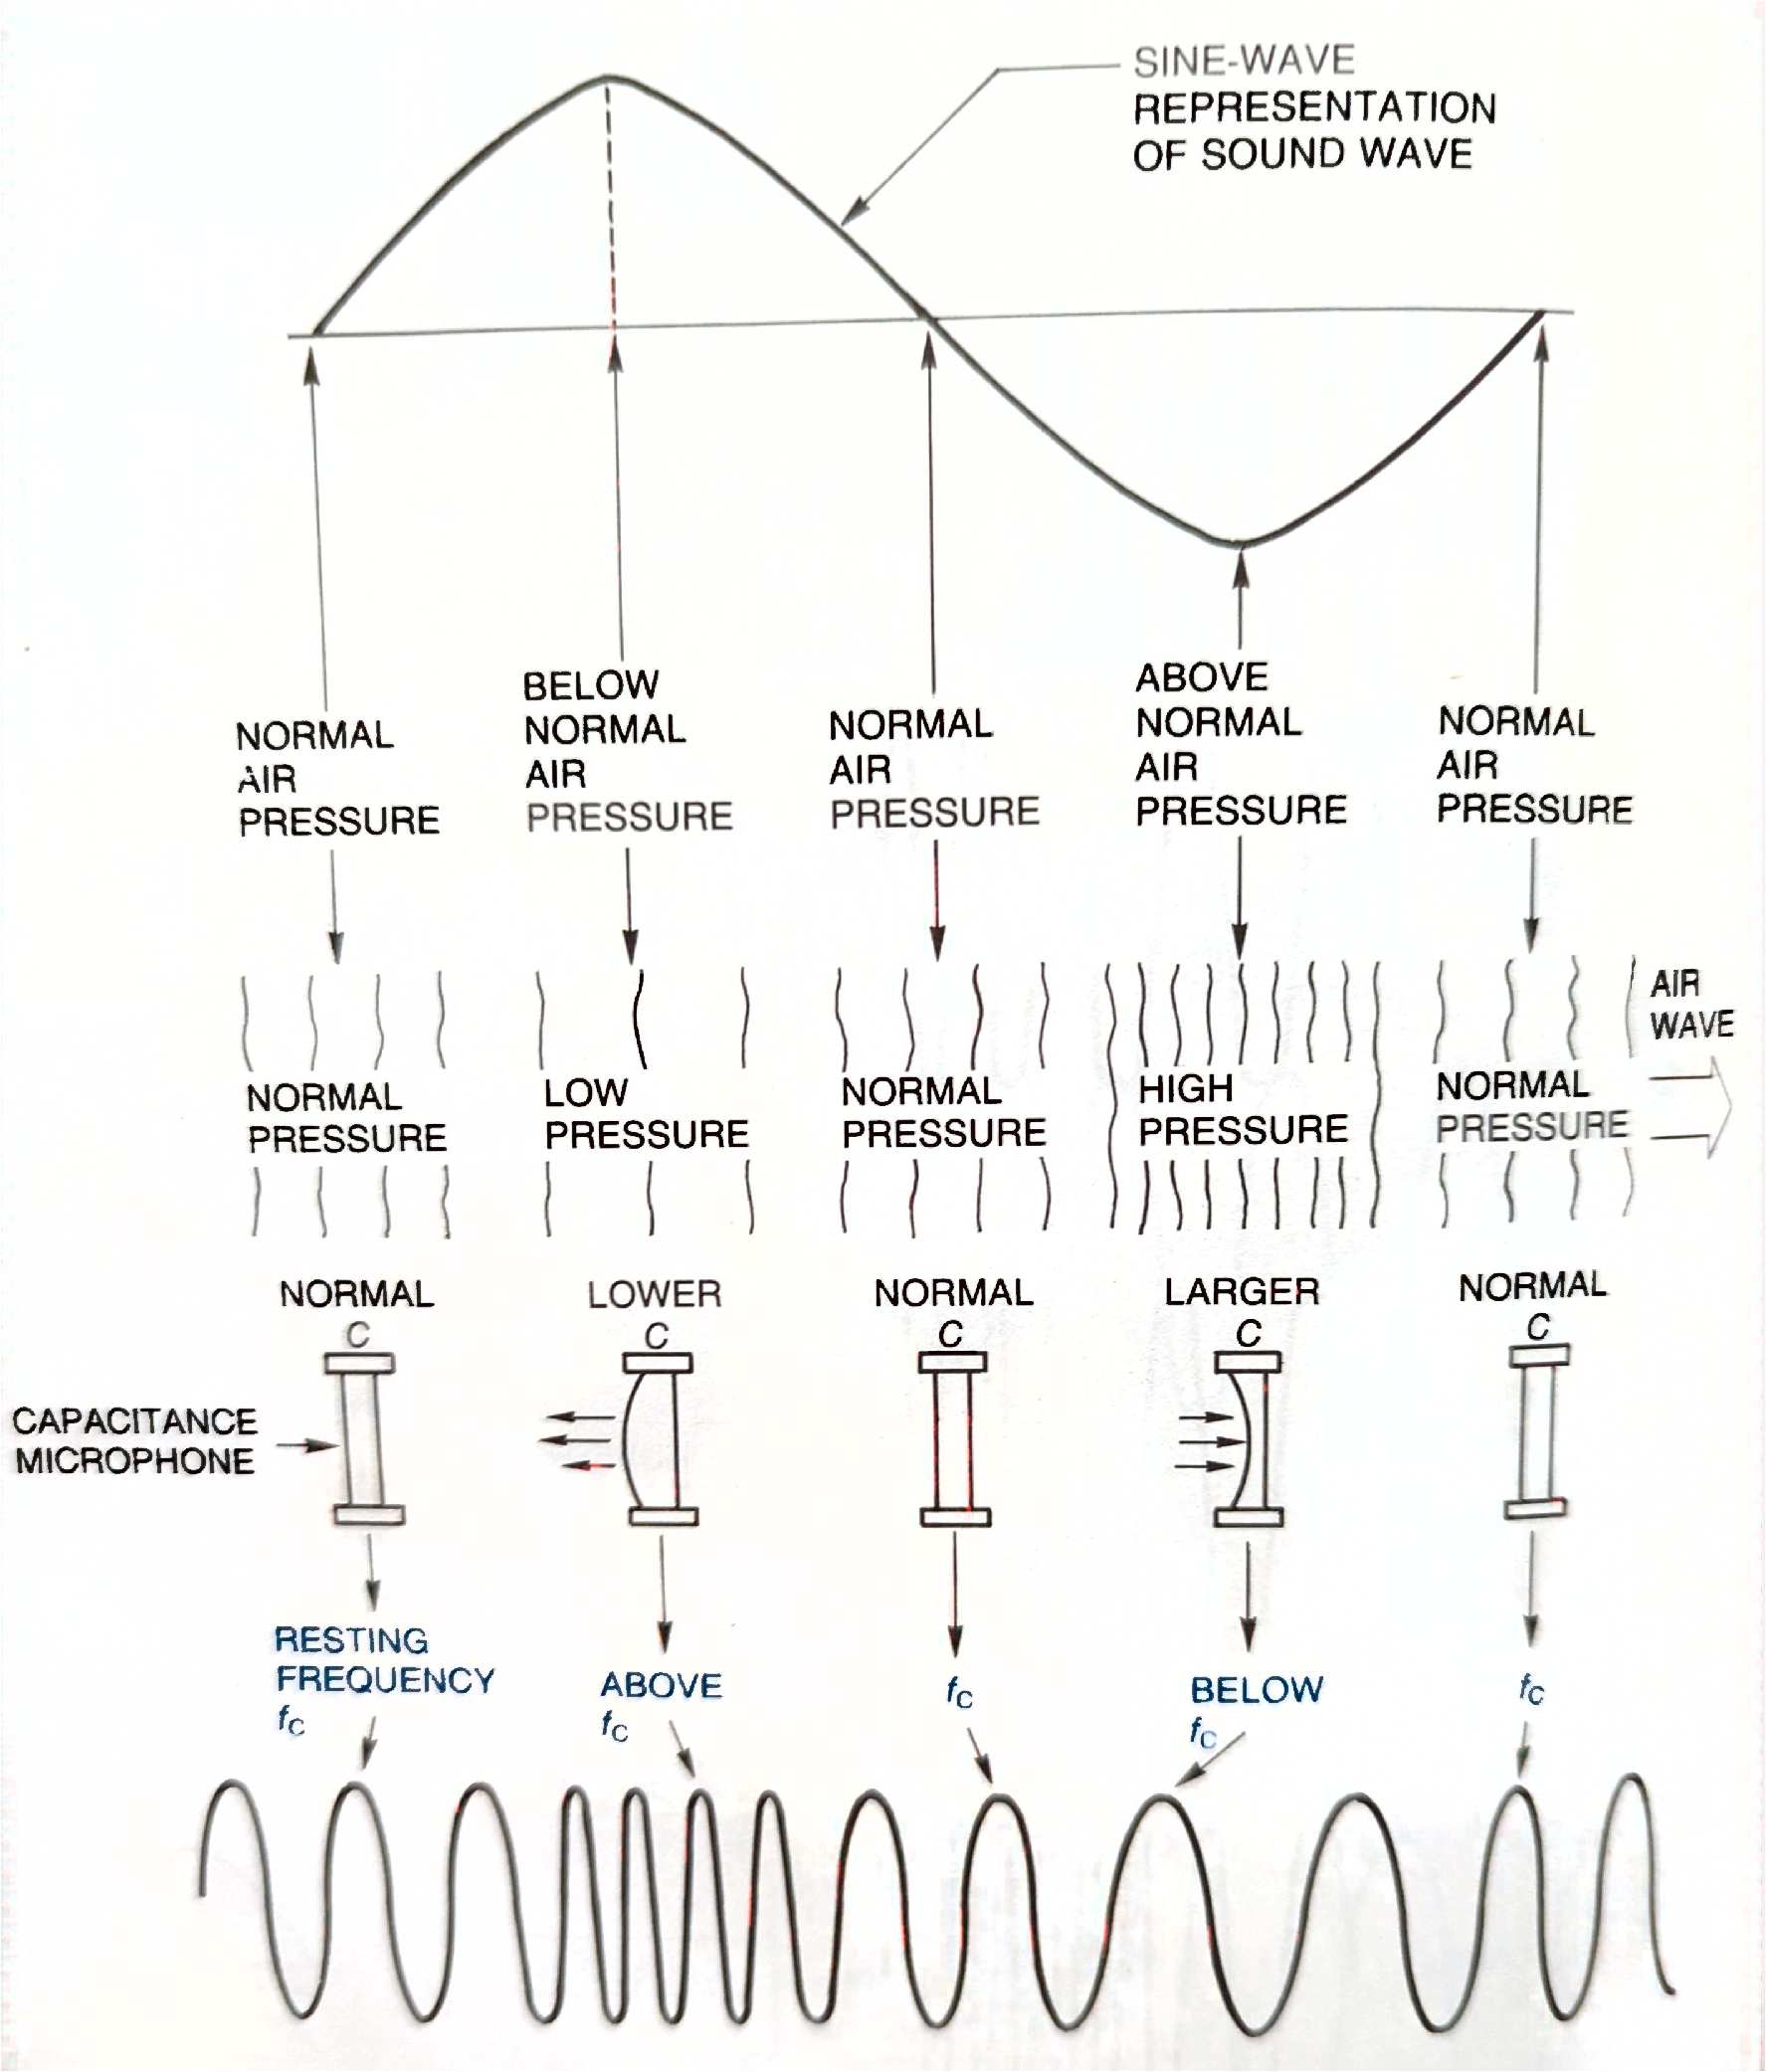
\includegraphics[width=0.475\textwidth]{figures/FMSpec3.pdf}
%\caption{\label{fig:radio3} \footnotesize (Left) Lowering $C$ raises $f_0$, and raising $C$ lowers $f_0$. (Right) Changes in pressure correspond to changes in $C$.}
%\end{figure}
%\end{frame}
%
%\begin{frame}{Electromagnetic waves: Electromagnetic spectrum and energy}
%\begin{columns}
%\begin{column}{0.5\textwidth}
%\small
%\textbf{\alert{In summary,}}
%\begin{enumerate}
%\item The $C$ in the LC oscillator can be made to depend on audio amplitude
%\item The audio amplitude corresponds to the frequency deviation
%\item The rate at which the frequency changes depends on audio frequency.
%\item \textbf{For those interested,} a great final project is to assemble a DIY AM transistor radio
%\end{enumerate}
%\end{column}
%\begin{column}{0.5\textwidth}
%\begin{figure}
%\centering
%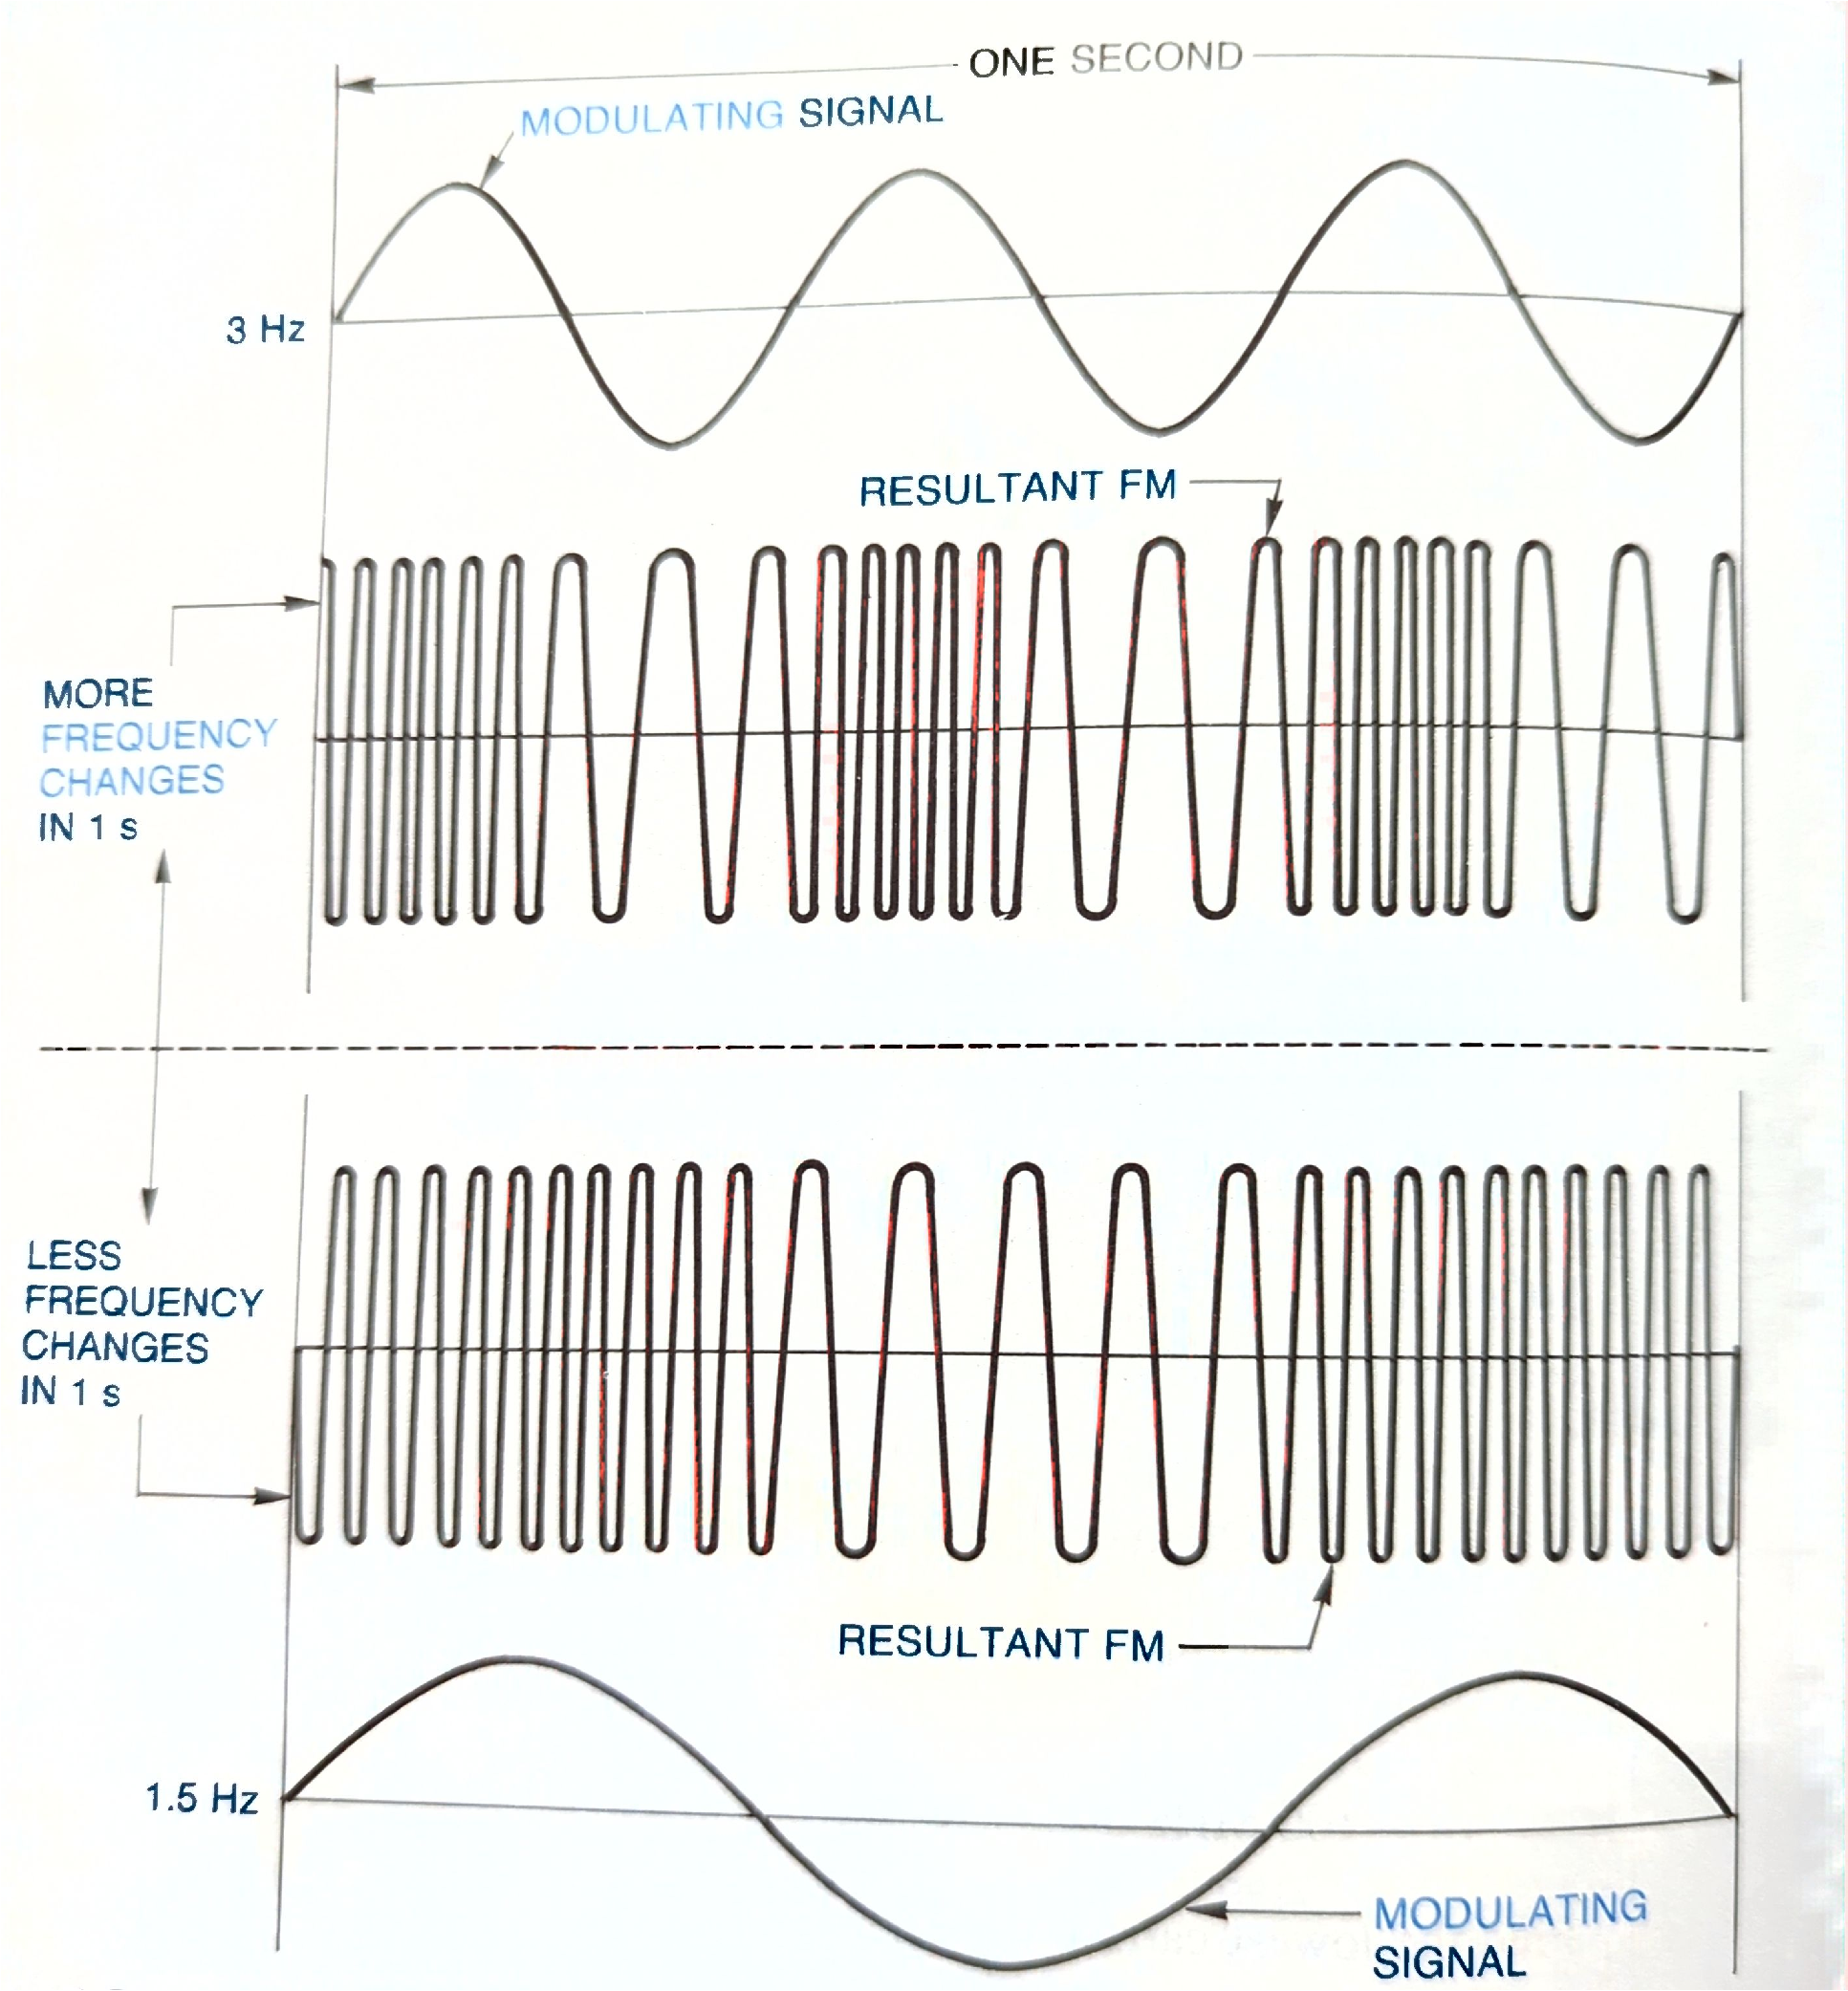
\includegraphics[width=0.95\textwidth]{figures/FMSpec4.pdf}
%\caption{\label{fig:radio4} \footnotesize Audio (modulation) frequency determines \textit{how often} the frequency deviates, not the frequency deviation itself.}
%\end{figure}
%\end{column}
%\end{columns}
%\end{frame}
%
%\begin{frame}{Unit 5 Summary}
%\begin{enumerate}
%\item Electromagnetic waves - \textbf{Chapters 24.1 - 24.4}
%\begin{itemize}
%\item Maxwell's Equations
%\item Electromagnetic wave production
%\item Electromagnetic spectrum and energy
%\end{itemize}
%\item Geometric optics - \textbf{Chapters 25.1 - 25.3, 25.6}
%\begin{itemize}
%\item Ray-tracing
%\item Reflection
%\item Refraction
%\item Lens optics
%\end{itemize}
%\end{enumerate}
%\end{frame}
%
%\begin{frame}{Unit 5 Summary}
%\begin{enumerate}
%\item Wave optics - \textbf{Chapters 27.1 - 27.3}
%\begin{itemize}
%\item Wave interference
%\item Wave diffraction
%\item Double slit experiments
%\end{itemize}
%\item Nuclear physics in medicine - \textbf{32.1 - 32.4}
%\begin{itemize}
%\item Diagnostics and medical imaging
%\item Biological effects of ionizing radiation
%\item Therapeutic uses of ionizing radiation
%\item Food irradiation
%\end{itemize}
%\end{enumerate}
%\end{frame}
%
%\section{Geometric optics: Ray-tracing and Reflection}
%
%\begin{frame}{Geometric optics: Ray-tracing and Reflection}
%\begin{figure}
%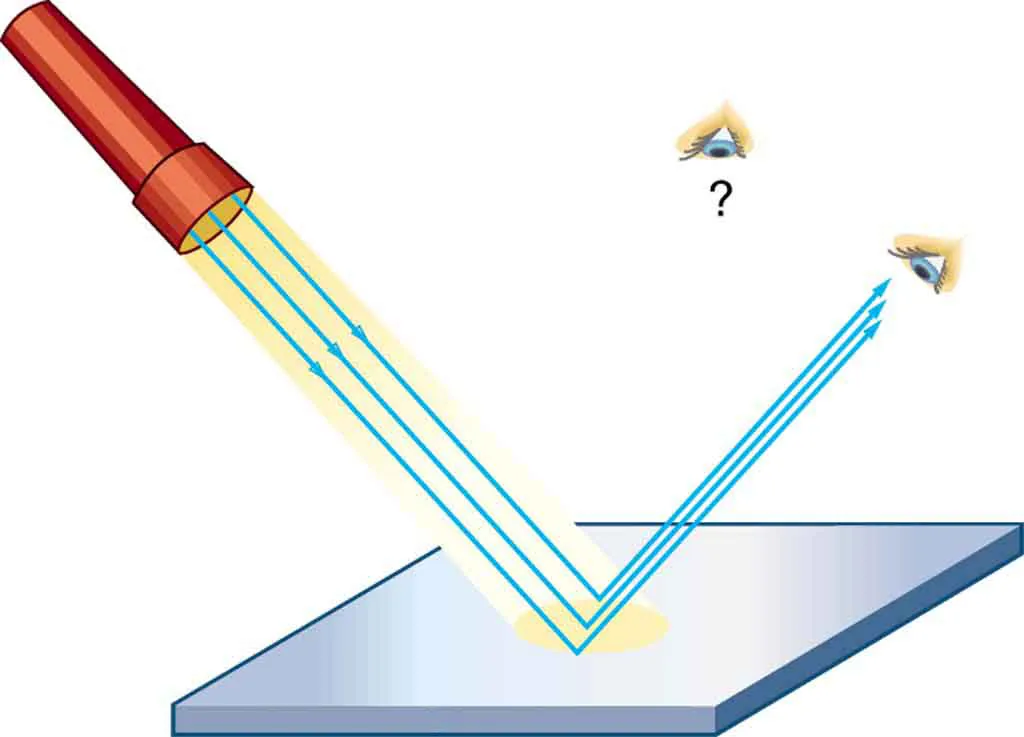
\includegraphics[width=0.375\textwidth]{figures/geo5.png}
%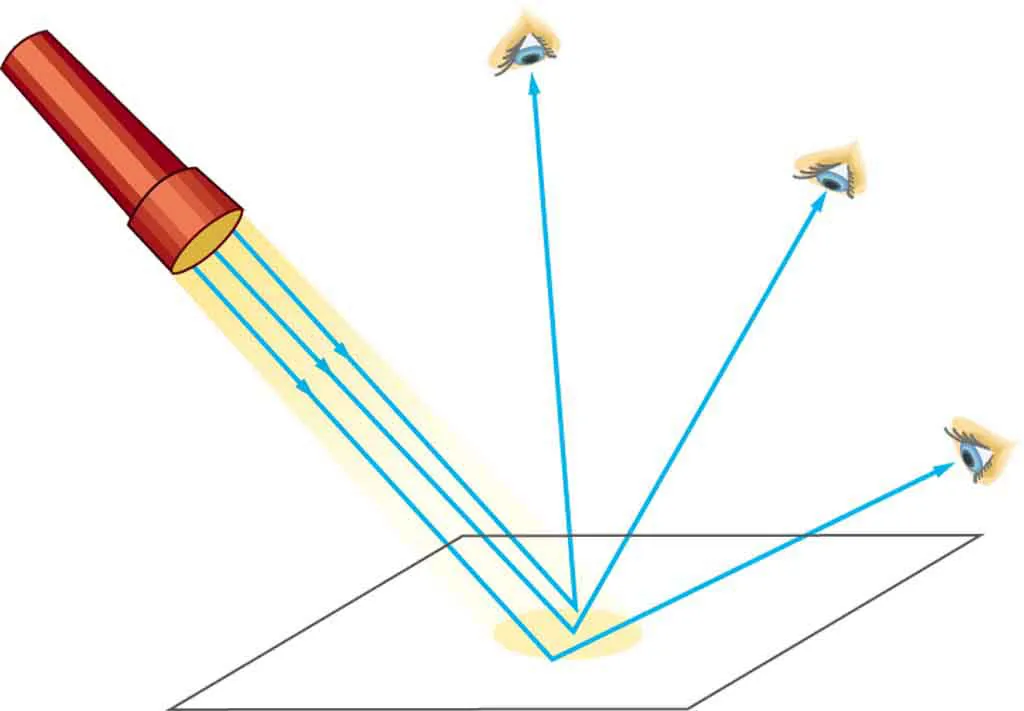
\includegraphics[width=0.375\textwidth]{figures/geo3.png}
%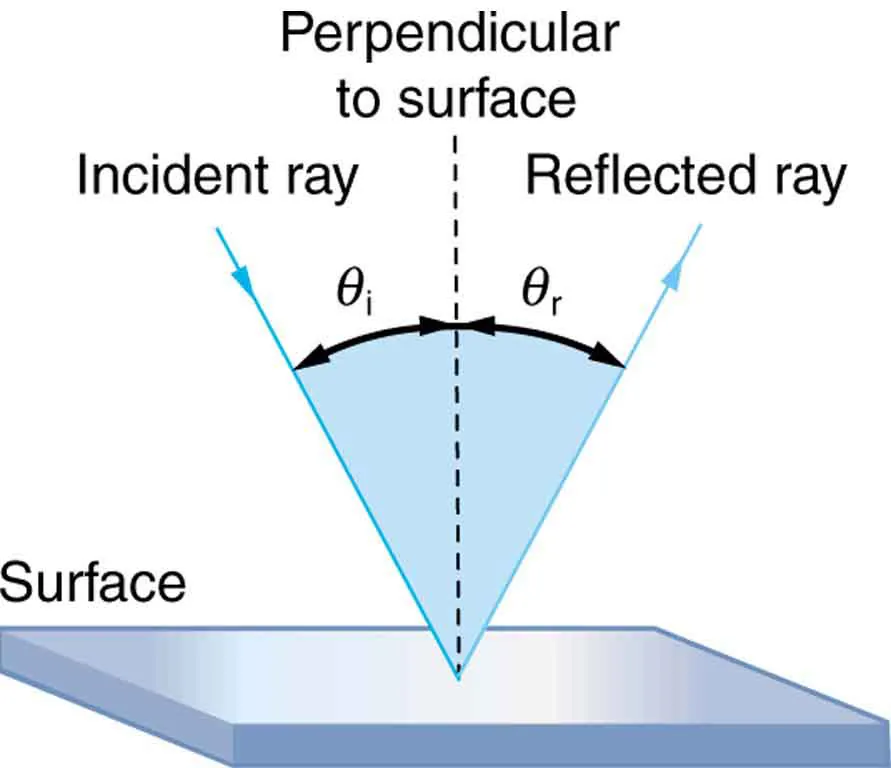
\includegraphics[width=0.375\textwidth]{figures/geo4.png}
%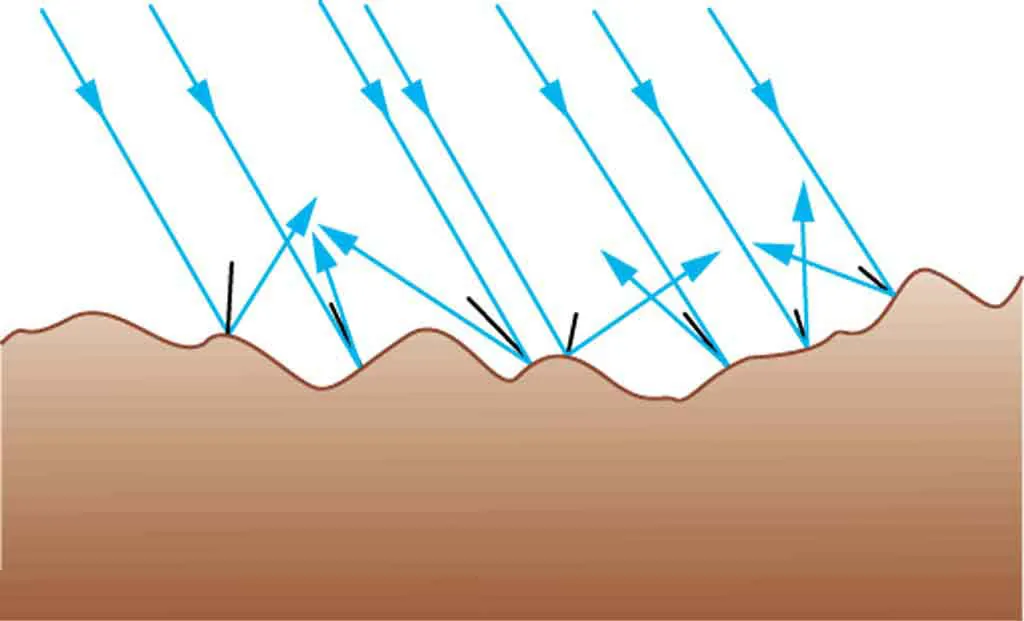
\includegraphics[width=0.375\textwidth]{figures/geo1.png}
%\caption{\label{fig:geo1} \footnotesize (Top left) Specular reflection (Top right) Diffuse reflection (Bottom left) Smooth surface (Bottom right) Rough surface.}
%\end{figure}
%\end{frame}
%
%\begin{frame}{Geometric optics: Ray-tracing and Reflection}
%\begin{figure}
%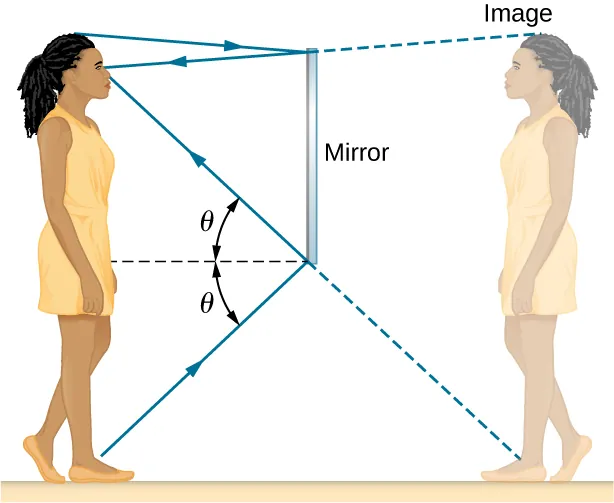
\includegraphics[width=0.375\textwidth]{figures/geo6.png}
%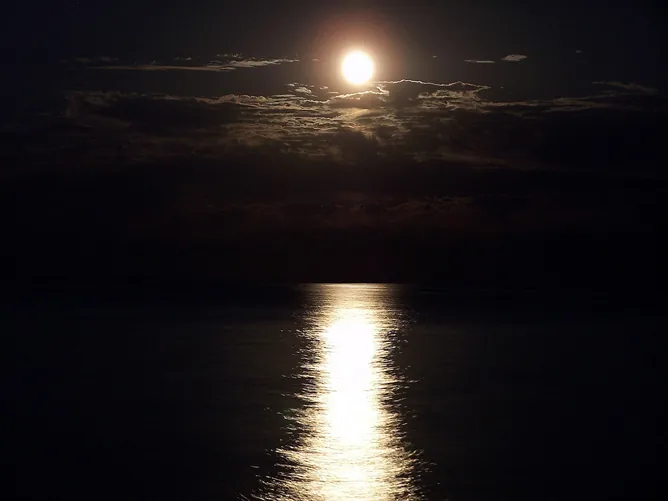
\includegraphics[width=0.375\textwidth]{figures/geo2.png}
%\caption{\label{fig:geo2} \footnotesize (Left) Your image in a mirror is due to specular reflection. (Right) The image of the moon on the ocean is due to diffuse reflection.}
%\end{figure}
%\small
%\textbf{\alert{Specular reflection}} rule: the incident angle and reflected angle are equal.
%\begin{equation}
%\theta_{\rm i} = \theta_{\rm r}
%\end{equation}
%Both angles are usually measured with respect to the direction orthogonal to the reflecting surface.
%\end{frame}
%
%\begin{frame}{Geometric optics: Ray-tracing and Reflection}
%\textbf{Group exercise:} Light shows staged with lasers use moving mirrors to swing beams and create colorful effects. Show that a light ray reflected from a mirror changes direction by $2\theta$ when the mirror is rotated by an angle $\theta$.
%\begin{figure}
%\centering
%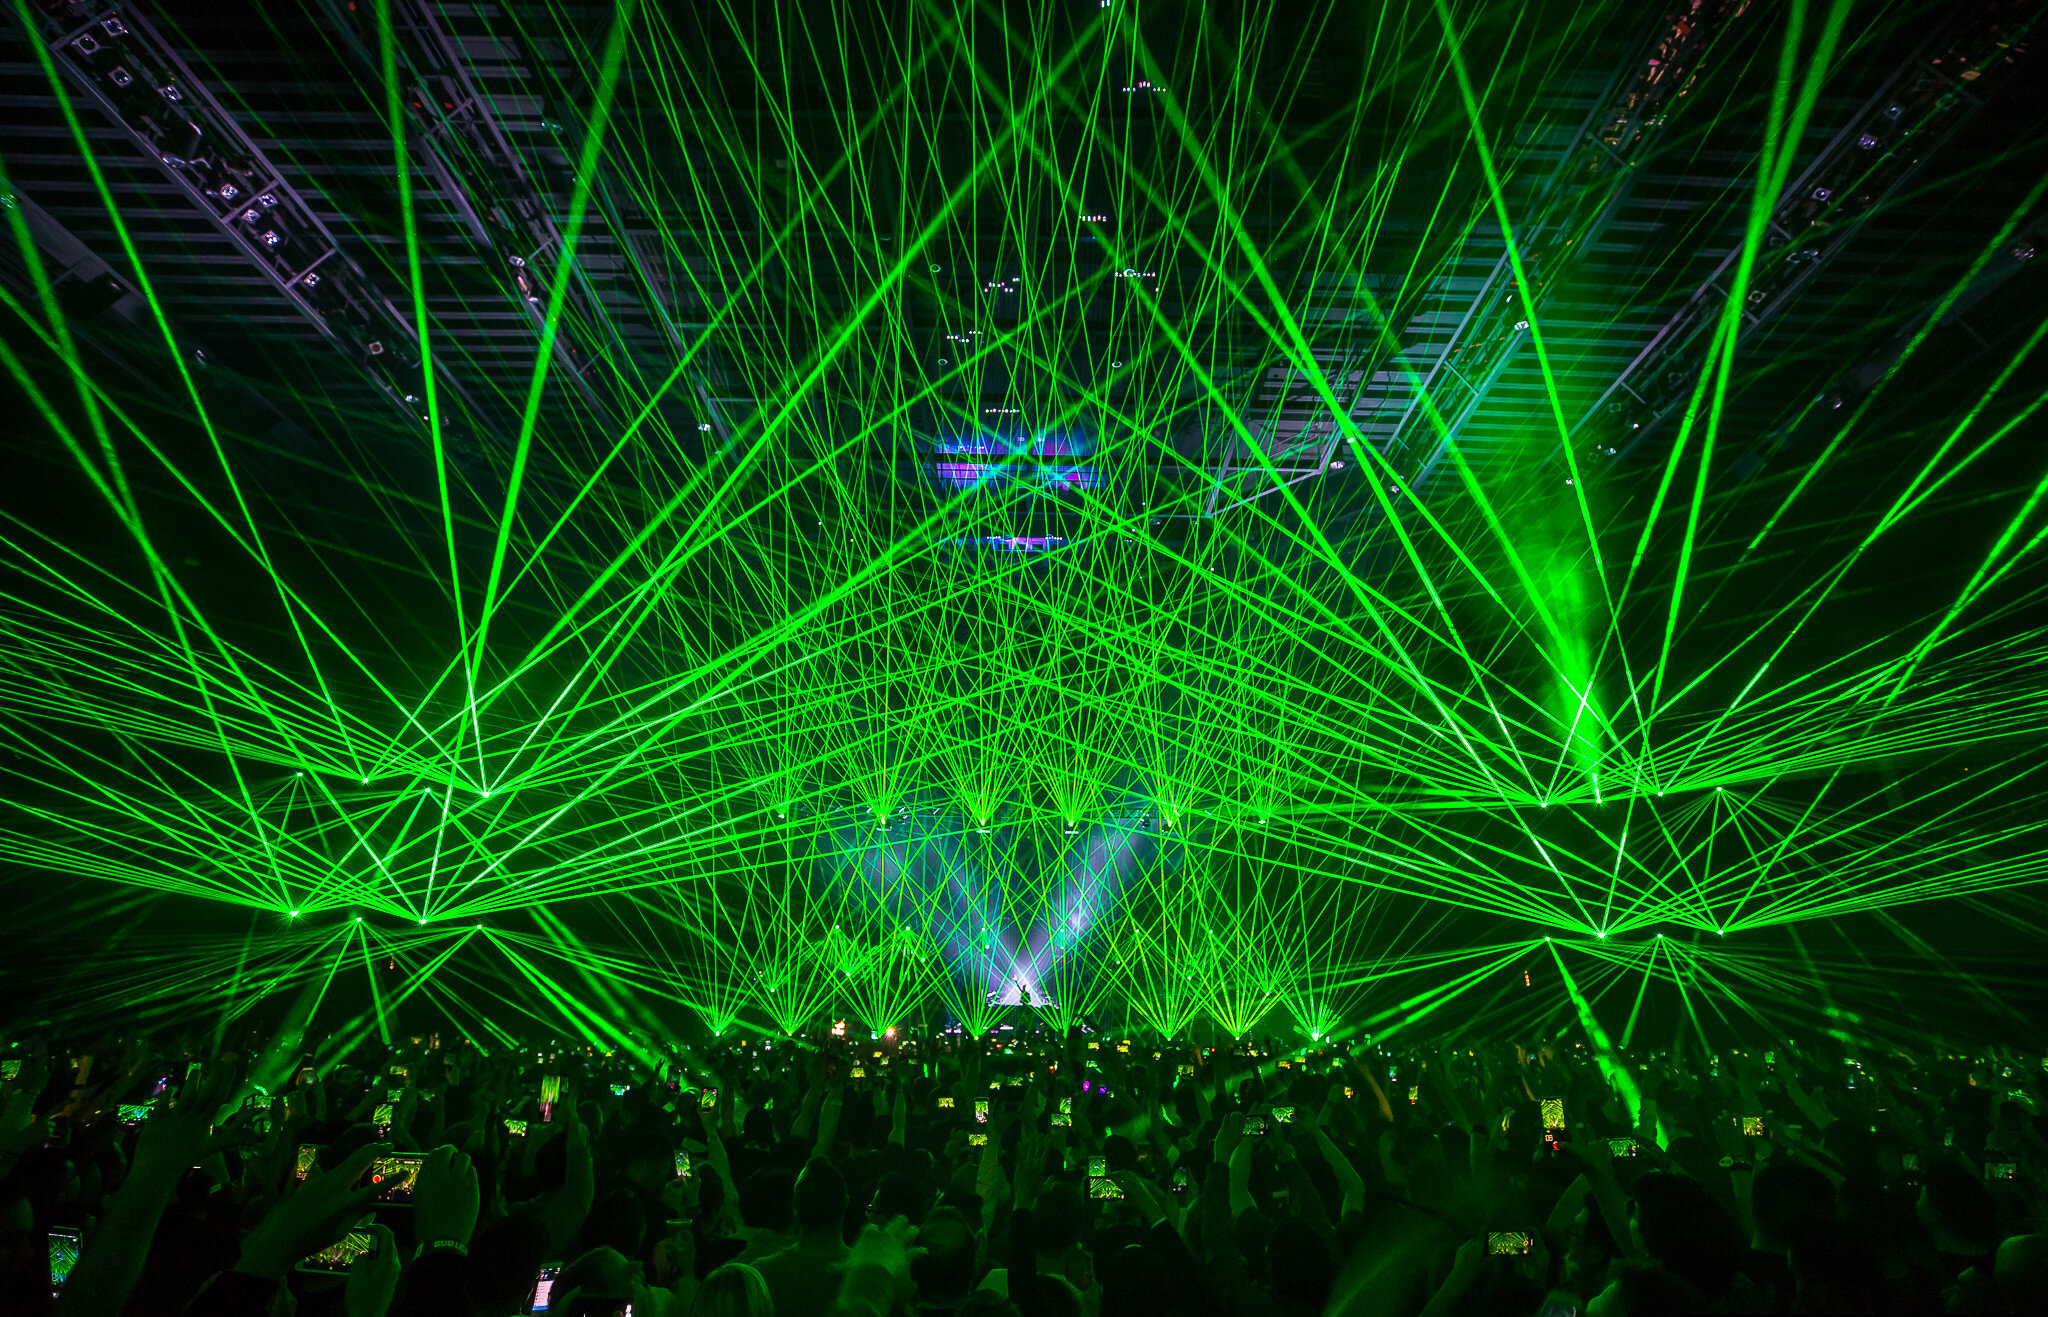
\includegraphics[width=0.45\textwidth]{figures/laserface.jpg}
%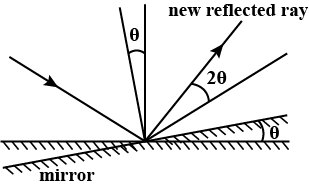
\includegraphics[width=0.45\textwidth]{figures/mirror.png}
%\end{figure}
%\footnotesize
%Think about rotating a mirror 90 degrees.  What happens to the reflected laser light?
%\end{frame}
%
%\begin{frame}{Geometric optics: Ray-tracing and Reflection}
%\small
%\textbf{\alert{The speed of light}} can be measured independently of electromagnetism, with an \textit{interferometer.}
%\begin{figure}
%\centering
%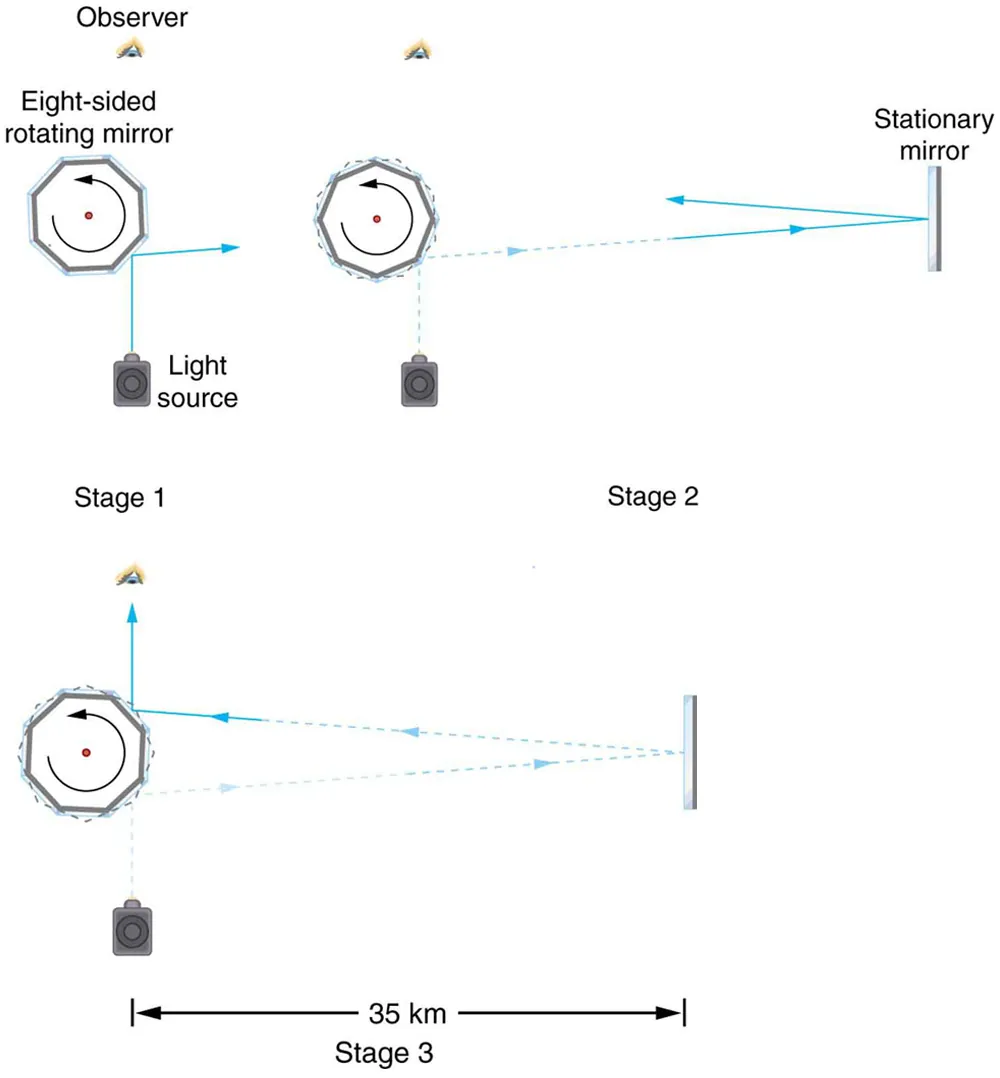
\includegraphics[width=0.45\textwidth]{figures/michelson.png}
%\caption{\label{fig:mich} A schematic of the 1887 experiment by Albert Michelson.}
%\end{figure}
%\end{frame}
%
%\begin{frame}{Geometric optics: Ray-tracing and Reflection}
%\begin{tcolorbox}[colback=white,colframe=black!40!black,title=The Speed of Light]
%\alert{The speed of light in a vacuum is
%\begin{equation}
%c = 2.99792458 \times 10^8~~m~s^{-1}
%\end{equation}
%When light travels through a material with \textit{index of \\ refraction, $n$}, the speed is
%\begin{equation}
%v = \frac{c}{n}
%\end{equation}
%}
%\end{tcolorbox}
%\end{frame}
%
%\begin{frame}{Geometric optics: Ray-tracing and Reflection}
%\textbf{In the Michelson interferometer}, light had to travel 35 km down to a mirror, and 35 km back from the mirror.  Assuming the speed of light in a vacuum ($3\times 10^8$ m/s), how long does it take for the light to make the round trip?
%\begin{itemize}
%\item A: 116 $\mu$s
%\item B: 116 ns
%\item C: 233 $\mu$s
%\item D: 233 ns
%\end{itemize}
%\end{frame}
%
%\begin{frame}{Geometric optics: Ray-tracing and Reflection}
%\textbf{In airborne radar}, aircraft must transmit a radio pulse and record the reflection time to determine the position of other aircraft.  If an aircraft records a reflection time of 700 $\mu$s, how far away is the object?
%\begin{itemize}
%\item A: 210 km
%\item B: 210 m
%\item C: 105 m
%\item D: 105 km
%\end{itemize}
%\end{frame}
%
%\begin{frame}{Geometric optics: Ray-tracing and Reflection}
%\textbf{\alert{The index of refraction}} is a property of materials and substances that depends on the atomic or molecular structure of electrons.
%\begin{table}
%\centering
%\begin{tabular}{| c | c | c |}
%\hline
%\textbf{Air} & Radio & 1.000368 \\ \hline
%\textbf{Air} & Optical & 1.000293 \\ \hline
%\textbf{Water, fresh} & Optical & 1.333 \\ \hline
%\textbf{Ice, fresh} & Optical & 1.31 \\ \hline
%\textbf{Ice, fresh} & Radio & 1.78 \\ \hline
%\end{tabular}
%\caption{\label{tab:n} Indices of refraction for several substances in different parts of the electromagnetic spectrum.}
%\end{table}
%\end{frame}
%
%\begin{frame}{Geometric optics: Ray-tracing and Reflection}
%\begin{table}
%\footnotesize
%\centering
%\begin{tabular}{| c | c | c |}
%\hline
%\textbf{Water, fresh} & Radio & 1.31 \\ \hline
%\textbf{Ice, fresh} & Radio & 1.78 \\ \hline
%\end{tabular}
%\caption{\label{tab:n2} \footnotesize Indices of refraction for several substances.}
%\end{table}
%\footnotesize
%Suppose we are measuring the ice shelf thickness in Greenland with \textbf{radio waves} to determine changes in ice volume due to climate change.  If in 2016 we observed a radio echo time of 1150 ns, and in 2020 we observed a time of 1125 ns, by how much has the ice thickness been reduced?
%\begin{itemize}
%\item A: 5.25 cm
%\item B: 52.5 cm
%\item C: 525 cm
%\item D: 0.525 cm
%\end{itemize}
%\footnotesize
%Hint: Assume the radio signal begins from the ice surface, travels down, and reflects from the bottom.
%\end{frame}
%
%\begin{frame}{Geometric optics: Ray-tracing and Reflection}
%\begin{tcolorbox}[colback=white,colframe=black!40!black,title=Reflection Coefficient at Normal Incidence]
%\alert{Suppose an electromagnetic wave in a medium with index of refraction $n_1$ approaches the surface of a medium with index of refraction $n_2$ at an angle $\theta_i = 0$ degrees.  The wave will be reflected at $\theta_r = 0$ degrees.  The \textbf{reflection coefficient} is the fraction of power or intensity reflected, and it is equal to
%\begin{equation}
%R = \left| \frac{n_1 - n_2}{n_1 + n_2}\right|^2
%\end{equation}
%The \textbf{transmission coefficient} is $T = 1 - R$, to conserve power and energy.
%}
%\end{tcolorbox}
%\end{frame}
%
%\begin{frame}{Geometric optics: Ray-tracing and Reflection}
%\begin{table}
%\footnotesize
%\centering
%\begin{tabular}{| c | c | c |}
%\hline
%\textbf{Water, fresh} & Radio & 1.31 \\ \hline
%\textbf{Ice, fresh} & Radio & 1.78 \\ \hline
%\end{tabular}
%\caption{\label{tab:n3} \footnotesize Indices of refraction for several substances.}
%\end{table}
%Suppose our aircraft radar is reflecting radar echos from a frozen lake surface.  Assuming air has $n_1 = 1.0$, what fraction of the power reflects from the lake?
%\begin{itemize}
%\item A: 100 percent
%\item B: 7.9 percent
%\item C: 15.8 percent
%\item D: 0 percent
%\end{itemize}
%\end{frame}
%
%\begin{frame}{Geometric optics: Ray-tracing and Reflection}
%\begin{table}
%\footnotesize
%\centering
%\begin{tabular}{| c | c | c |}
%\hline
%\textbf{Water, fresh} & Radio & 1.31 \\ \hline
%\textbf{Ice, fresh} & Radio & 1.78 \\ \hline
%\end{tabular}
%\caption{\label{tab:n4} \footnotesize Indices of refraction for several substances.}
%\end{table}
%If we cross from a region of ice to fresh water, what is the new result?
%\begin{itemize}
%\item A: 100 percent
%\item B: 3.6 percent
%\item C: 1.8 percent
%\item D: 0 percent
%\end{itemize}
%\end{frame}
%
%\begin{frame}{Geometric optics: Ray-tracing and Reflection}
%\begin{figure}
%\centering
%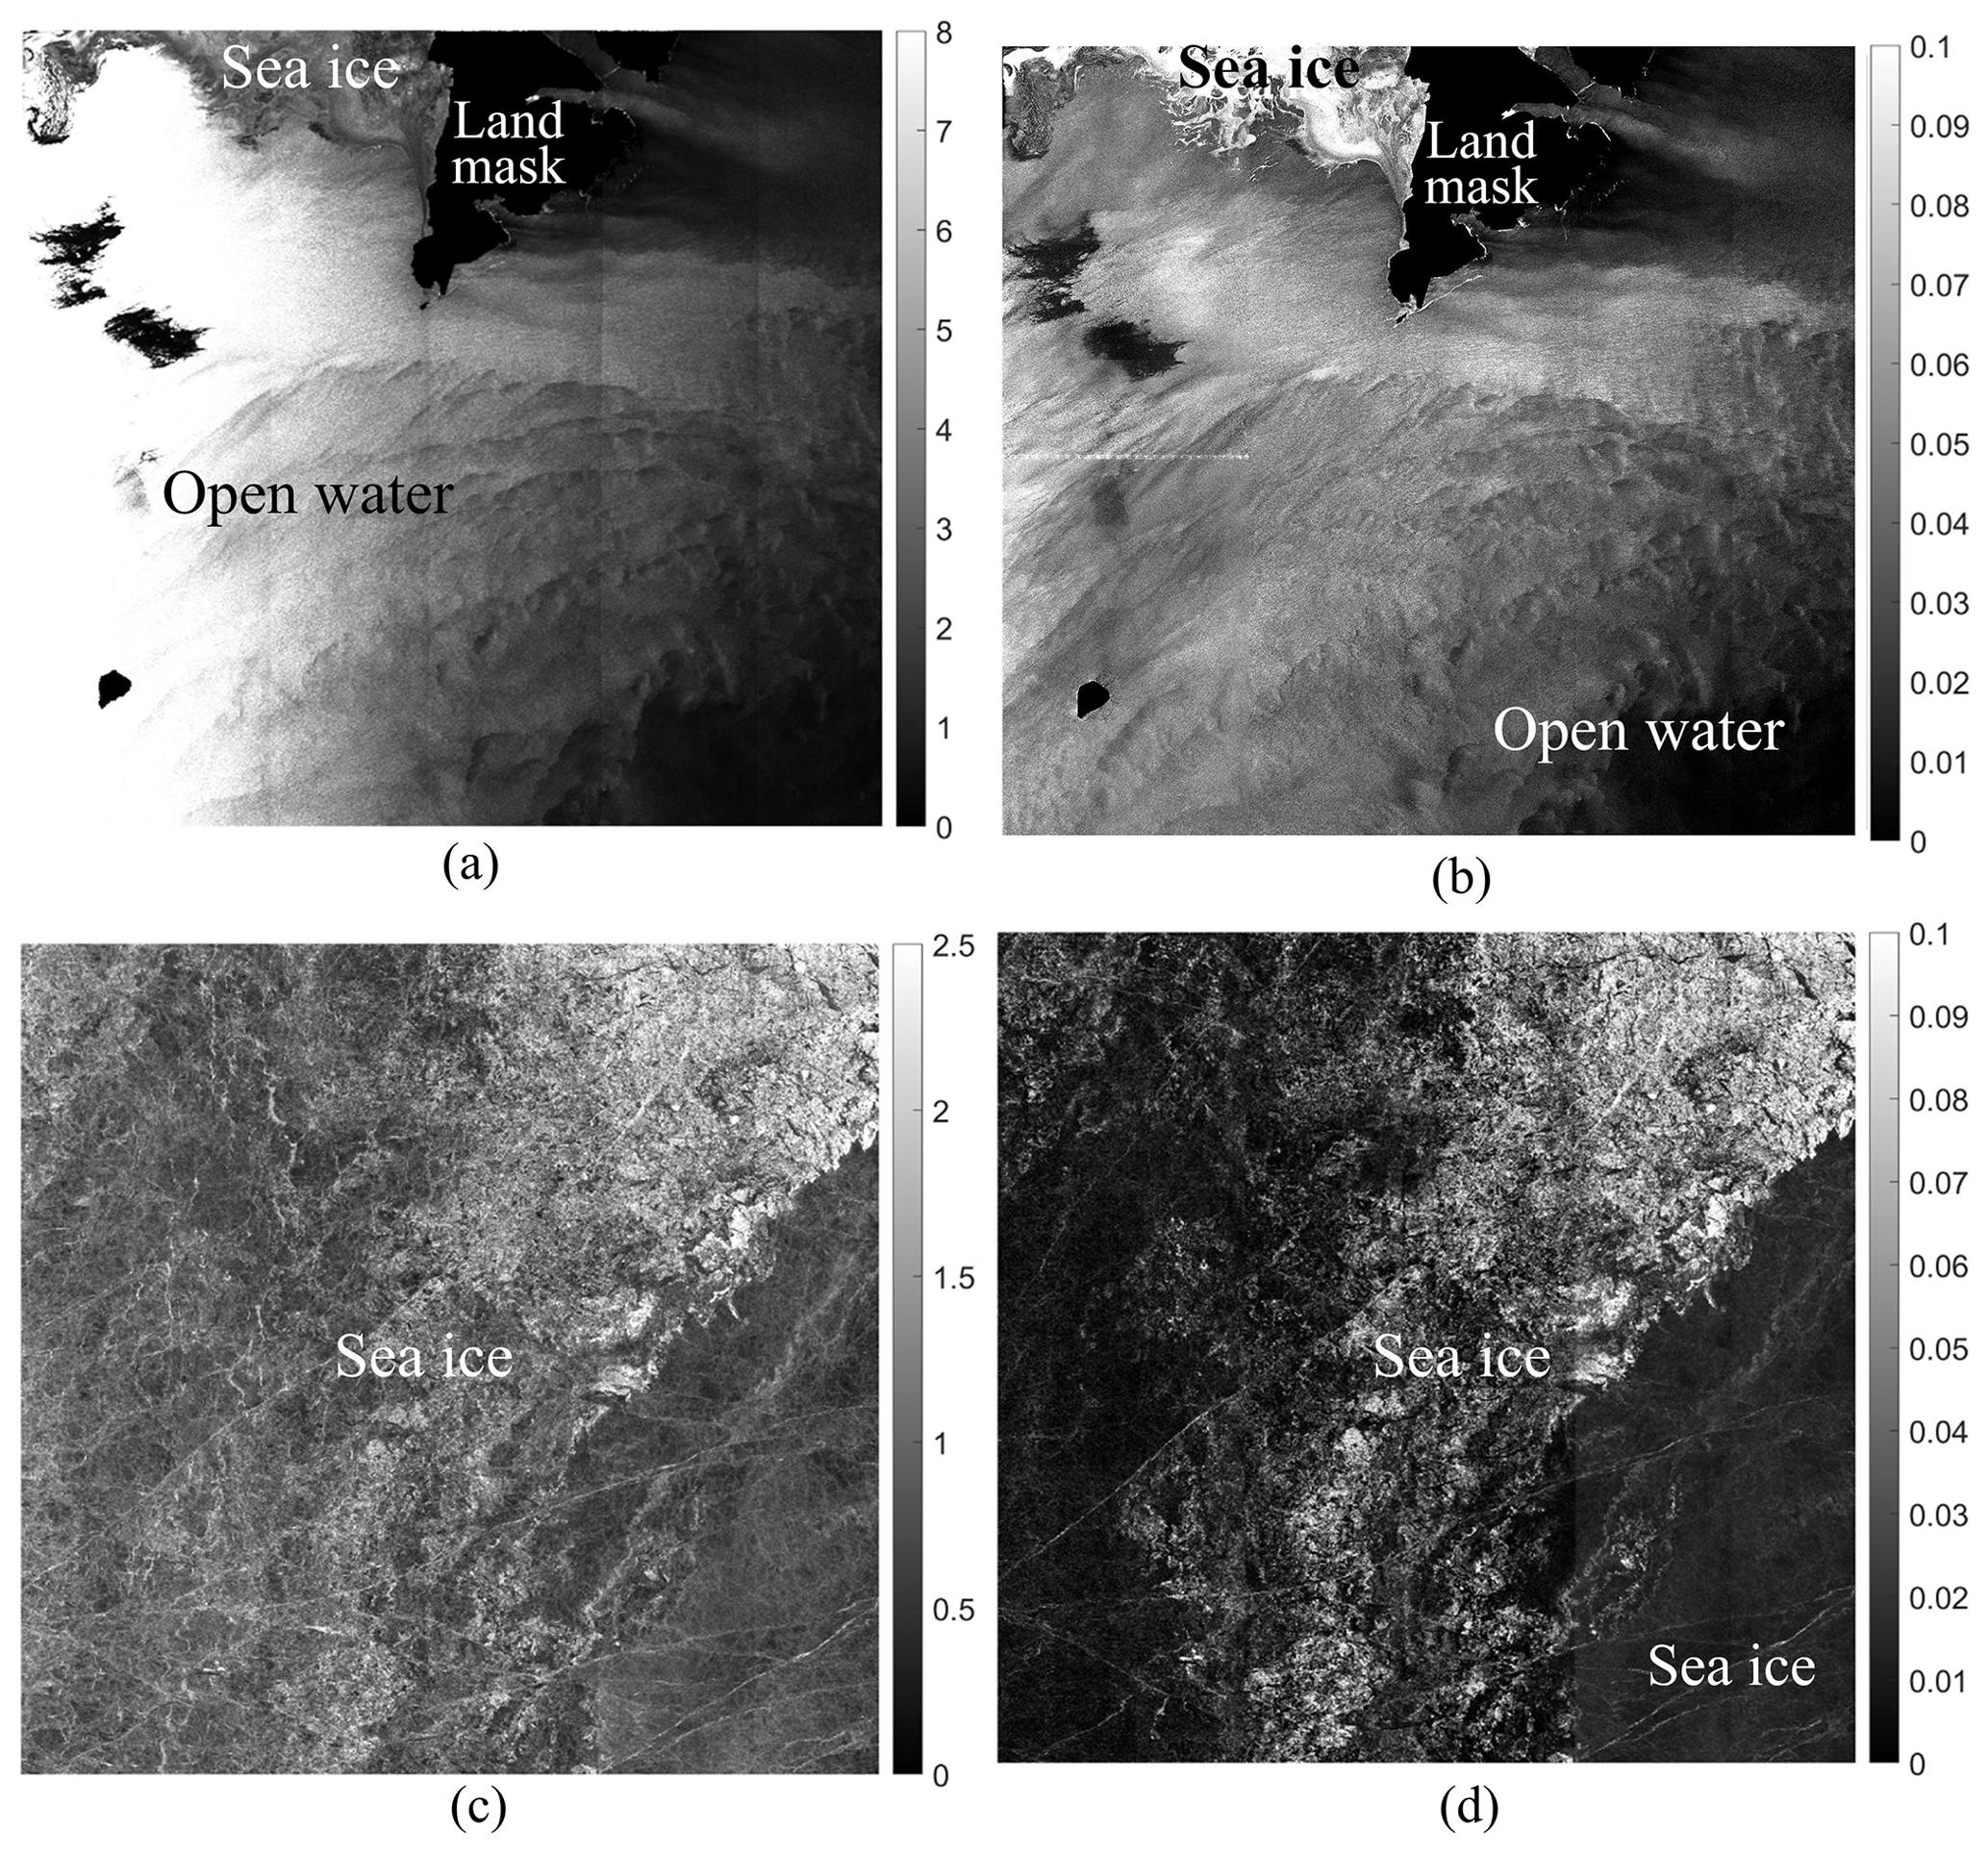
\includegraphics[width=0.6\textwidth]{figures/sea_ice.png}
%\caption{\label{fig:sea} \footnotesize A result from Wang and Li, ``Arctic sea ice cover data from spaceborne synthetic aperture radar by deep learning.'' Earth System Science Data \textbf{13}(6) 2723-2742, 2021.}
%\end{figure}
%\end{frame}
%
%\section{PhET: Geometric optics and Reflection Coefficients}
%
%\begin{frame}{PhET: Geometric optics and Reflection Coefficients}
%Navigate to \url{https://phet.colorado.edu/en/simulations/bending-light} \\
%\begin{enumerate}
%\item Click on the More Tools tab, and drag the laser tool to the top so that the light experiences normal incidence.
%\item Activate the laser tool by clicking the red button.  The reflected light appears above the laser tool.
%\item Use the green intensity tool at left to measure the reflected intensity.
%\item Measure the reflection coefficient between air and water by controlling the indices with the sliders at right.
%\item Copy your result into 100 spreadsheet cells \textbf{in Google Sheets} ($2 \to 4 \to 8 \to ...$).
%\end{enumerate}
%\end{frame}
%
%\begin{frame}[fragile]{PhET: Geometric optics and Reflection Coefficients}
%Navigate to \url{https://phet.colorado.edu/en/simulations/bending-light} \\
%\begin{enumerate}
%\item Suppose your data exist in A1:A100.  In cell B1, type the following:
%\begin{verbatim}
%=NORMINV(RAND(),A1,0.01)
%\end{verbatim}
%\item The previous step will create a \textit{gaussian random error} with the mean of A1 and standard deviation of 0.01.
%\item In cell C1, enter a number that is a few tenths of a percent below the average reflection coefficient (e.g. 3.9).  Then, in cell C2, write:
%\begin{verbatim}
%=C1+0.01
%\end{verbatim}
%\item Click and drag C2 until the C-cells encompass the range of data we find in column B (e.g [3.9:4.1]).
%\end{enumerate}
%\end{frame}
%
%\begin{frame}[fragile]{PhET: Geometric optics and Reflection Coefficients}
%Navigate to \url{https://phet.colorado.edu/en/simulations/bending-light} \\
%\begin{enumerate}
%\item Assume the column C cells we created exist in C1:C21.  In cell D1, type the following:
%\begin{verbatim}
%=FREQUENCY(B1:B100,C1:C21)
%\end{verbatim}
%\item Now hit CNTL+Shift+Enter.  The formula will be encapsulated by \verb+ArrayFormula+, and hit enter until the \verb+FREQUENCY+ function is evaluated.
%\item The results are \textit{frequencies} in the sense that, next to each frequency bin, the function calculates \textit{how frequently} data fall into the given bin.
%\item Create an x-y scatter graph of frequency bins (column C) versus frequencies (column D).
%\end{enumerate}
%\end{frame}
%
%\begin{frame}[fragile]{PhET: Geometric optics and Reflection Coefficients}
%Navigate to \url{https://phet.colorado.edu/en/simulations/bending-light} \\
%\begin{enumerate}
%\item This type of chart is called a \textit{histogram.}
%\item Does your histogram peak at the expected reflection coefficient?
%\item What does the width of your histogram tell you?
%\end{enumerate}
%\end{frame}
%
%\section{Geometric optics: Refraction}
%
%\begin{frame}[fragile]{PhET: Geometric optics and Refraction}
%\footnotesize
%Navigate to \url{https://phet.colorado.edu/en/simulations/bending-light} \\
%\begin{enumerate}
%\item Perhaps you noticed in the previous activity that transmission angle depends on both $n_2$ and $\theta_i$.  We will now sort out that relationship.
%\item Click on the More Tools tab, and click on the yellow protractor at left.
%\item Place the center of the protractor at the spot where the laser hits the surface.
%\item Select $n_1 = 1.0$, and $n_2 = 1.5$.  Take 15-20 data points of $\theta_i$ and $\theta_t$, where $\theta_i$ is the incident angle with respect to normal, and $\theta_t$ is the transmission angle with respect to normal.
%\item Graph $\theta_t$ vs. $\theta_i$.  Do you observe a linear effect?
%\item Now graph $\sin\theta_t$ vs. $\sin\theta_i$.  Do you observe a linearized trend?
%\item Infer a general rule based on your data.
%\end{enumerate}
%\end{frame}
%
%\begin{frame}[fragile]{Geometric optics: Refraction}
%\begin{tcolorbox}[colback=white,colframe=black!40!black,title=Snell's Law]
%\alert{Let two media have two indices of refraction, $n_1$ and $n_2$, and let $\theta_i$ and $\theta_t$ represent the incident and transmission angles, measured with respect to normal.  Snell's Law relates these quantities:
%\begin{equation}
%n_1 \sin\theta_i = n_2\sin\theta_t
%\end{equation}
%}
%\end{tcolorbox}
%\end{frame}
%
%\begin{frame}[fragile]{Geometric optics: Refraction}
%Suppose you see your friend swimming underwater, and you are standing in the water near them.  Are they:
%\begin{itemize}
%\item A: Farther away than they appear
%\item B: Exactly where they appear
%\item C: Closer than they appear
%\item D: Deeper than they appear
%\end{itemize}
%\end{frame}
%
%\begin{frame}[fragile]{Geometric optics: Refraction}
%\begin{figure}
%\centering
%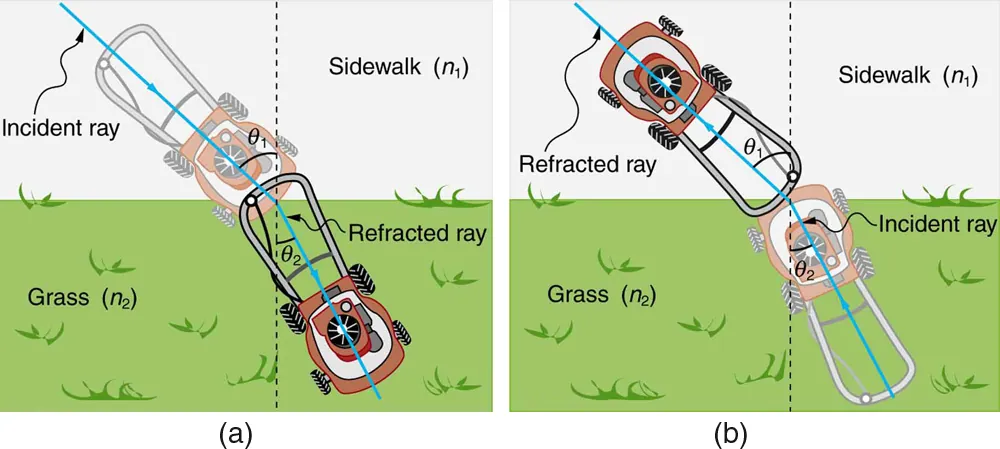
\includegraphics[width=0.65\textwidth]{figures/mower.png}
%\caption{\label{fig:mower} (a) The mower crosses from sidewalk to grass. (b) The mower crosses from grass to sidewalk.}
%\end{figure}
%\footnotesize
%The mower is powered by the two back wheels, and the speed they generate depends on the torque of the motor and axel against the surface.  This speed is higher on the sidewalk than the grass.  If the mower enters the grass at an angle, the right side goes slower before the left side.  The right side goes faster first as the mower enters the sidewalk.
%\end{frame}
%
%\begin{frame}{Geometric optics: Refraction}
%\begin{columns}[T]
%\begin{column}{0.5\textwidth}
%\begin{figure}
%\centering
%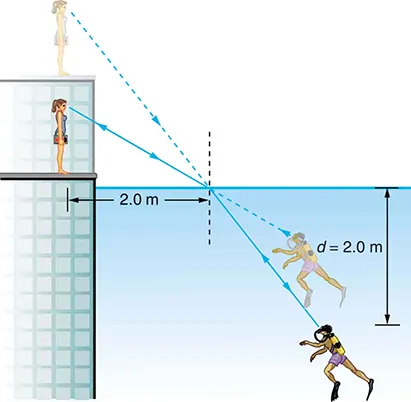
\includegraphics[width=0.95\textwidth]{figures/scuba.png}
%\caption{\label{fig:scuba2} \footnotesize A scuba diver is 2.0 m beneath the water surface ($n=1.3$).}
%\end{figure}
%\end{column}
%\begin{column}{0.5\textwidth}
%\footnotesize
%A scuba diver looks at his instructor.  What angle does the ray from the instructor’s face make with respect to normal at the point where the ray enters? The angle between the ray in the water and normal is 25.0 degrees.
%\begin{itemize}
%\item A: 15.2 degrees
%\item B: 25.0 degrees
%\item C: 30.1 degrees
%\item D: 34.3 degrees
%\end{itemize}
%\end{column}
%\end{columns}
%\end{frame}
%
%\begin{frame}{Geometric optics: Refraction}
%\begin{columns}[T]
%\begin{column}{0.5\textwidth}
%\begin{figure}
%\centering
%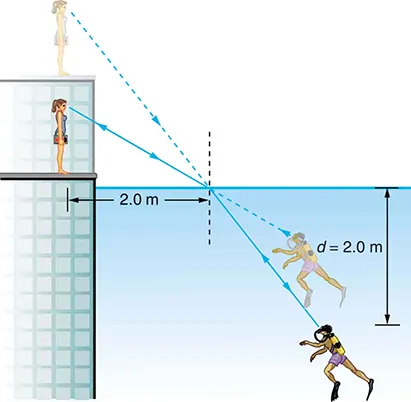
\includegraphics[width=0.95\textwidth]{figures/scuba.png}
%\caption{\label{fig:scuba3} \footnotesize A scuba diver is 2.0 m beneath the water surface ($n=1.3$).}
%\end{figure}
%\end{column}
%\begin{column}{0.5\textwidth}
%\footnotesize
%A scuba diver looks at his instructor.  How tall is the instructor?
%\begin{itemize}
%\item A: 1.23 meters
%\item B: 4.56 meters
%\item C: 7.89 meters
%\item D: 2.93 meters
%\end{itemize}
%\footnotesize Hint: draw your own diagram.
%\end{column}
%\end{columns}
%\footnotesize
%\textbf{\alert{Is your answer reasonable?}}
%\end{frame}
%
%\begin{frame}{Geometric optics: Refraction}
%\begin{columns}[T]
%\begin{column}{0.5\textwidth}
%\begin{figure}
%\centering
%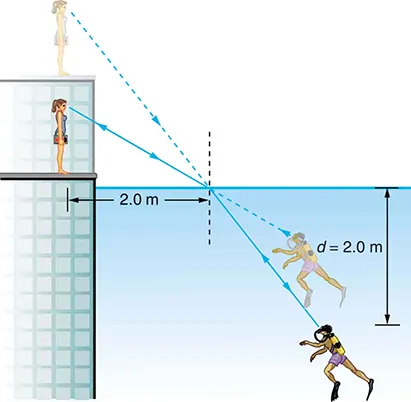
\includegraphics[width=0.95\textwidth]{figures/scuba.png}
%\caption{\label{fig:scuba4} \footnotesize A scuba diver is 2.0 m beneath the water surface ($n=1.3$).}
%\end{figure}
%\end{column}
%\begin{column}{0.5\textwidth}
%The answer was 2.93 meters.  No.  It really is, according to the Instructor's Solutions Manual. \\
%
\includegraphics[width=0.75\textwidth]{figures/idk.jpg}
%\end{column}
%\end{columns}
%\footnotesize
%\textbf{For reference}: there is a lens simulator at \url{https://phet.colorado.edu/en/simulations/geometric-optics}.
%\end{frame}
%
%\section{Geometric optics: Lens optics}
%
%\begin{frame}{Geometric optics: Lens optics}
%\textbf{\alert{Lens optics}} provides an understanding of image formation by lenses given the laws of refraction and lens properties.
%\begin{figure}
%\centering
%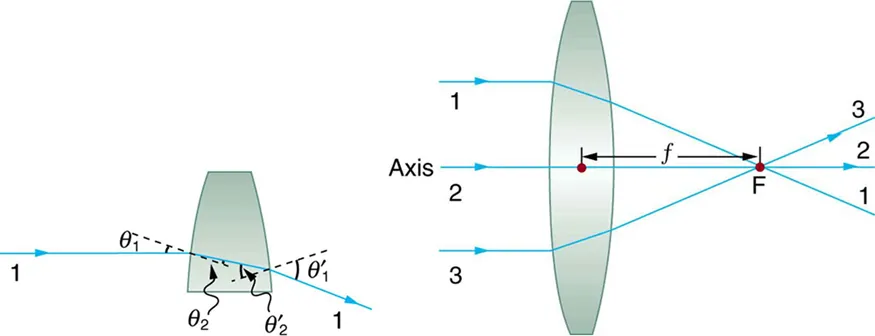
\includegraphics[width=0.45\textwidth,trim=13.5cm 0cm 0cm 0cm,clip=true]{figures/lens.png}
%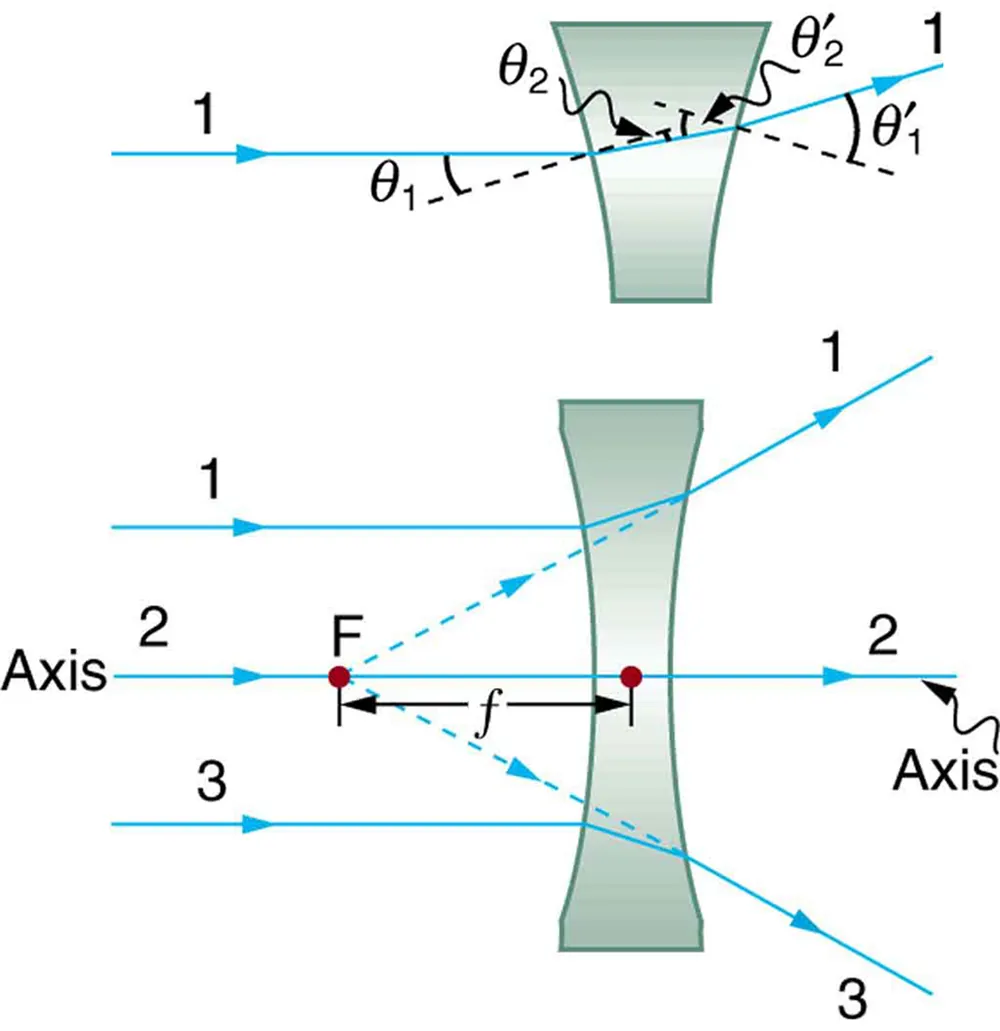
\includegraphics[width=0.45\textwidth,trim=0cm 0cm 0cm 11.5cm,clip=true]{figures/lens2.png}
%\caption{\label{fig:lens} (Left) A converging lens. (Right) A diverging lens.}
%\end{figure}
%\small
%The \textit{focal length, f} is the distance from the lens center where rays converge (converging lenses), or from where rays appear to diverge (diverging lenses).
%\end{frame}
%
%\begin{frame}{Geometric optics: Lens optics}
%\begin{figure}
%\centering
%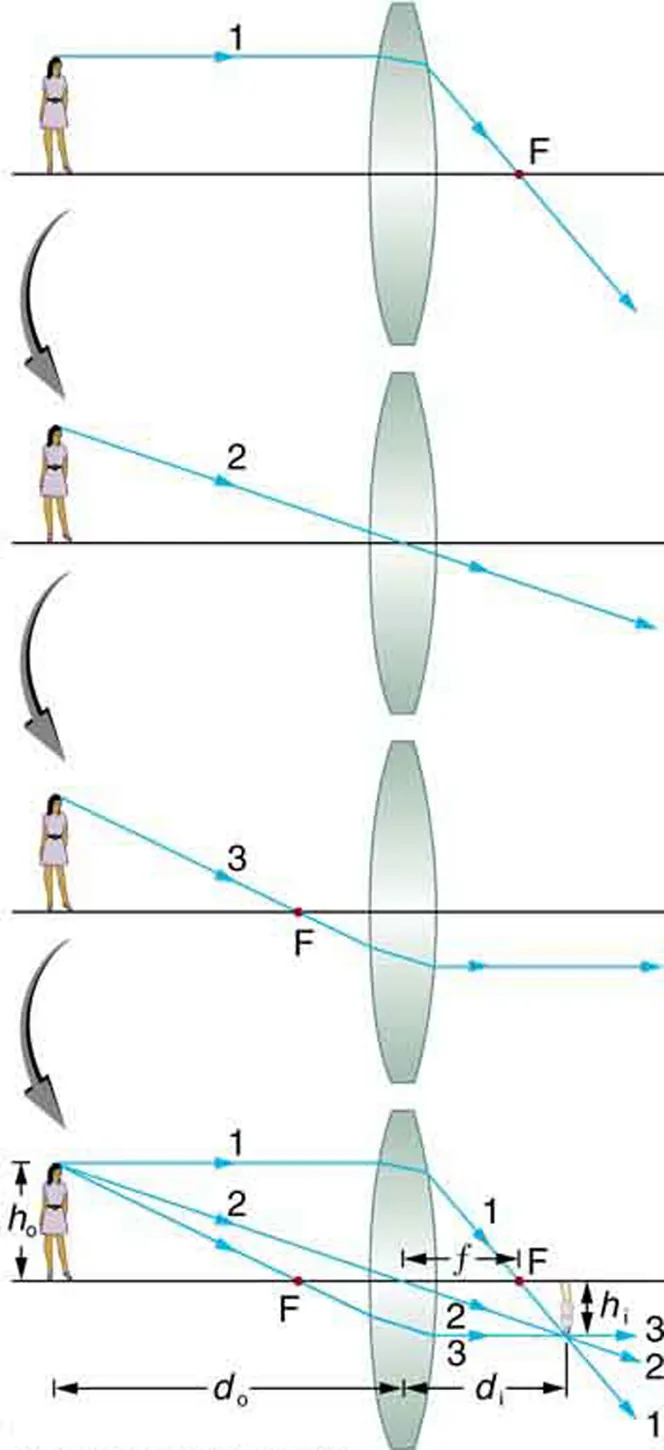
\includegraphics[width=0.45\textwidth,trim=0cm 26cm 0cm 0cm,clip=true]{figures/thin_lens.png}
%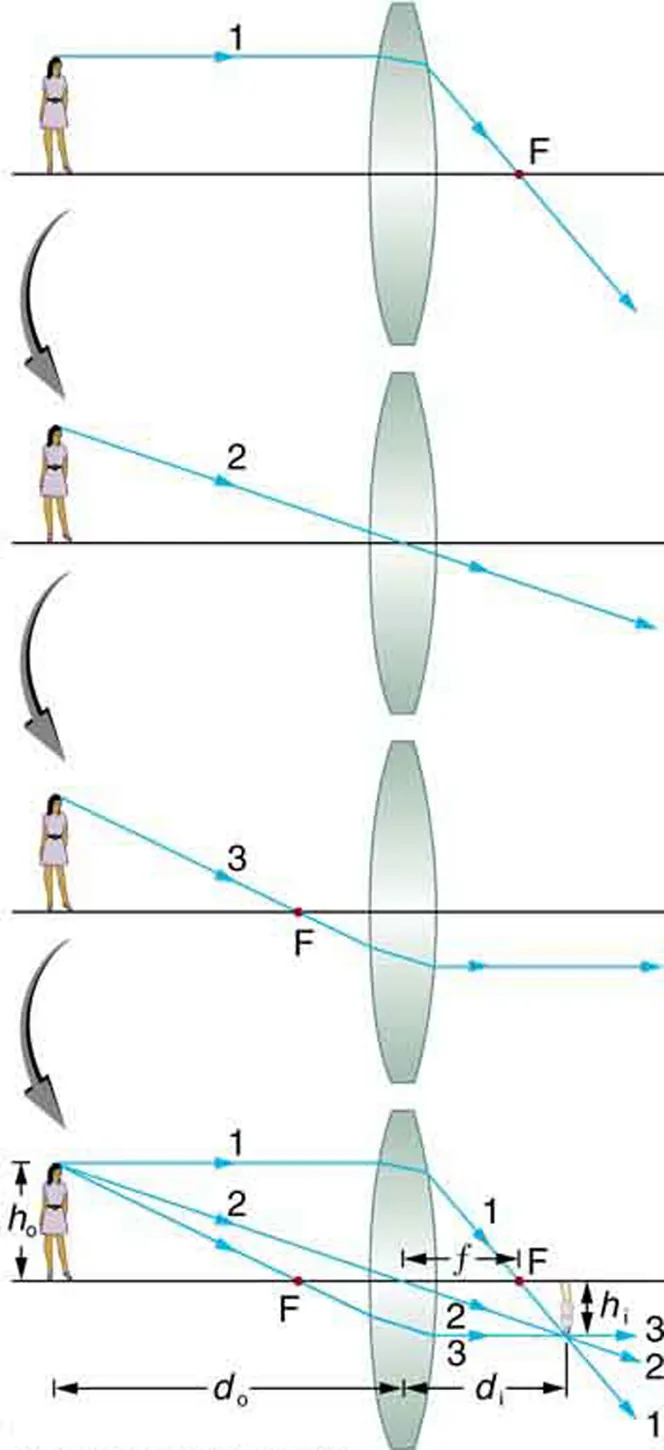
\includegraphics[width=0.45\textwidth,trim=0cm 0cm 0cm 26cm,clip=true]{figures/thin_lens.png}
%\caption{\label{fig:lens2} \small Rays 1, 2, and 3, pass parallel through the lens, through the center of the lens, and through the lens focal length, respectively.  A \textbf{real image} is formed on the other side.}
%\end{figure}
%\end{frame}
%
%\begin{frame}{Geometric optics: Lens optics}
%\begin{tcolorbox}[colback=white,colframe=black!40!black,title=Thin Lens Equations]
%\alert{Let $d_o$ be the distance from the source to the lens center.  Let $d_i$ be the distance from the lens center to the real image.  Let $f$ be the focal length.  Let $h_o$ be the object height.  let $h_i$ be the real image height.  The thin lens approximation gives
%\begin{align}
%\frac{1}{d_o} + \frac{1}{d_i} &= \frac{1}{f} \\
%m = \frac{h_i}{h_o} &= -\frac{d_i}{d_o}
%\end{align}
%The ratio $m$ is called the \textbf{magnification.}
%}
%\end{tcolorbox}
%\end{frame}
%
%\begin{frame}{Geometric optics: Lens optics}
%\begin{columns}[T]
%\begin{column}{0.5\textwidth}
%Suppose we have a lens with $f = 3$ cm.  Where will the image be if $d_o = 10$ m?
%\begin{itemize}
%\item A: 0 cm
%\item B: 3 cm
%\item C: 10 cm
%\item D: 10 m
%\end{itemize}
%\end{column}
%\begin{column}{0.5\textwidth}
%For the same lens, what is the magnification?
%\begin{itemize}
%\item A: $-3 \times 10^{0}$
%\item B: $3 \times 10^{-1}$
%\item C: $3 \times 10^{-2}$
%\item D: $-3 \times 10^{-3}$
%\end{itemize}
%\end{column}
%\end{columns}
%\end{frame}
%
%\begin{frame}{Geometric optics: Lens optics}
%\begin{columns}[T]
%\begin{column}{0.5\textwidth}
%Why was the magnification so small in the prior example?
%\begin{itemize}
%\item A: The object was close to the lens
%\item B: The object was far from the lens
%\item C: The object was at the focal length
%\item D: The object was within the focal length
%\end{itemize}
%\end{column}
%\begin{column}{0.5\textwidth}
%Suppose $d_o = 10$ cm, and $f = 3$ cm.  What are $d_i$ and $m$?
%\begin{itemize}
%\item A: $30/7$ cm, $-3/7$
%\item B: $30$ cm, $-1/2$
%\item C: $7/30$, $-3/7$ cm
%\item D: $30/7$, $-3/7$
%\end{itemize}
%What happens if $d_o = f$?
%\begin{itemize}
%\item A: $d_i = f$
%\item B: $d_i = 0$
%\item C: $d_i \to \infty$
%\item D: $d_0 = 1/f$
%\end{itemize}
%\end{column}
%\end{columns}
%\end{frame}
%
%\begin{frame}{Geometric optics: Lens optics}
%\textbf{\alert{An object within the focal length}} creates a \textit{virtual image}.
%\begin{figure}
%\centering
%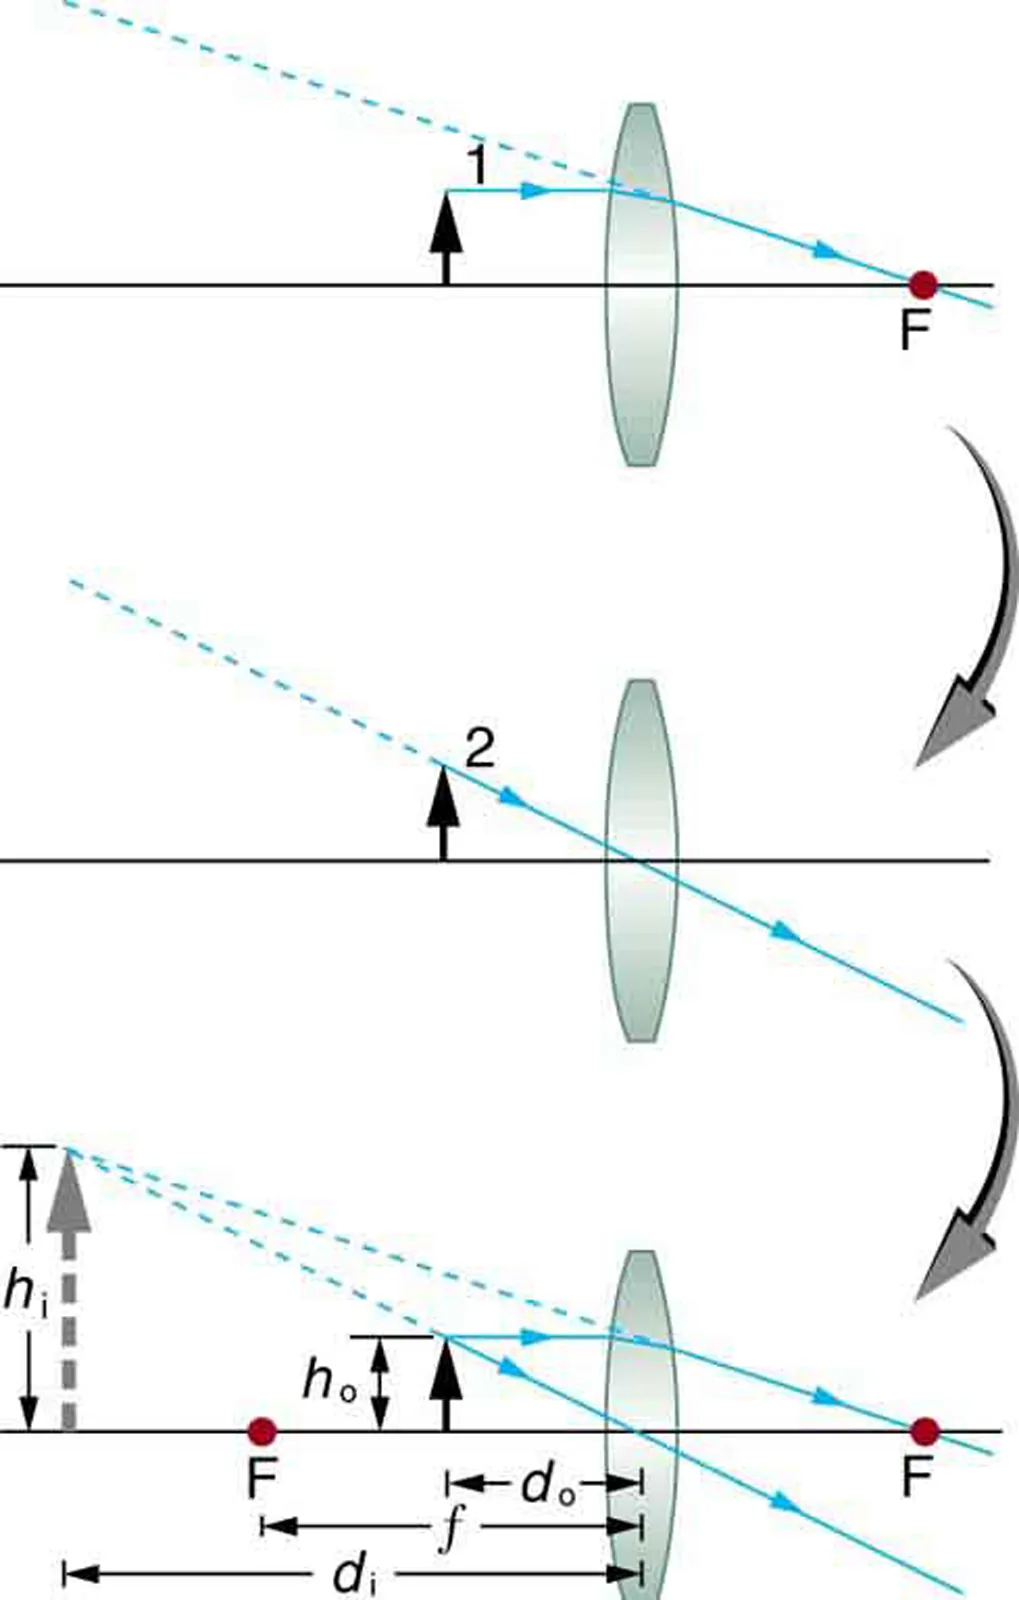
\includegraphics[width=0.3\textwidth]{figures/virtual.png}
%\caption{\label{fig:lens3} \small Rays 1 and 2 pass parallel through the lens to the focal point, and through the lens center, respectively.  A \textbf{virtual image} forms on the same side.}
%\end{figure}
%\end{frame}
%
%\begin{frame}{Geometric optics: Lens optics}
%\begin{columns}[T]
%\begin{column}{0.5\textwidth}
%\begin{figure}
%\centering
%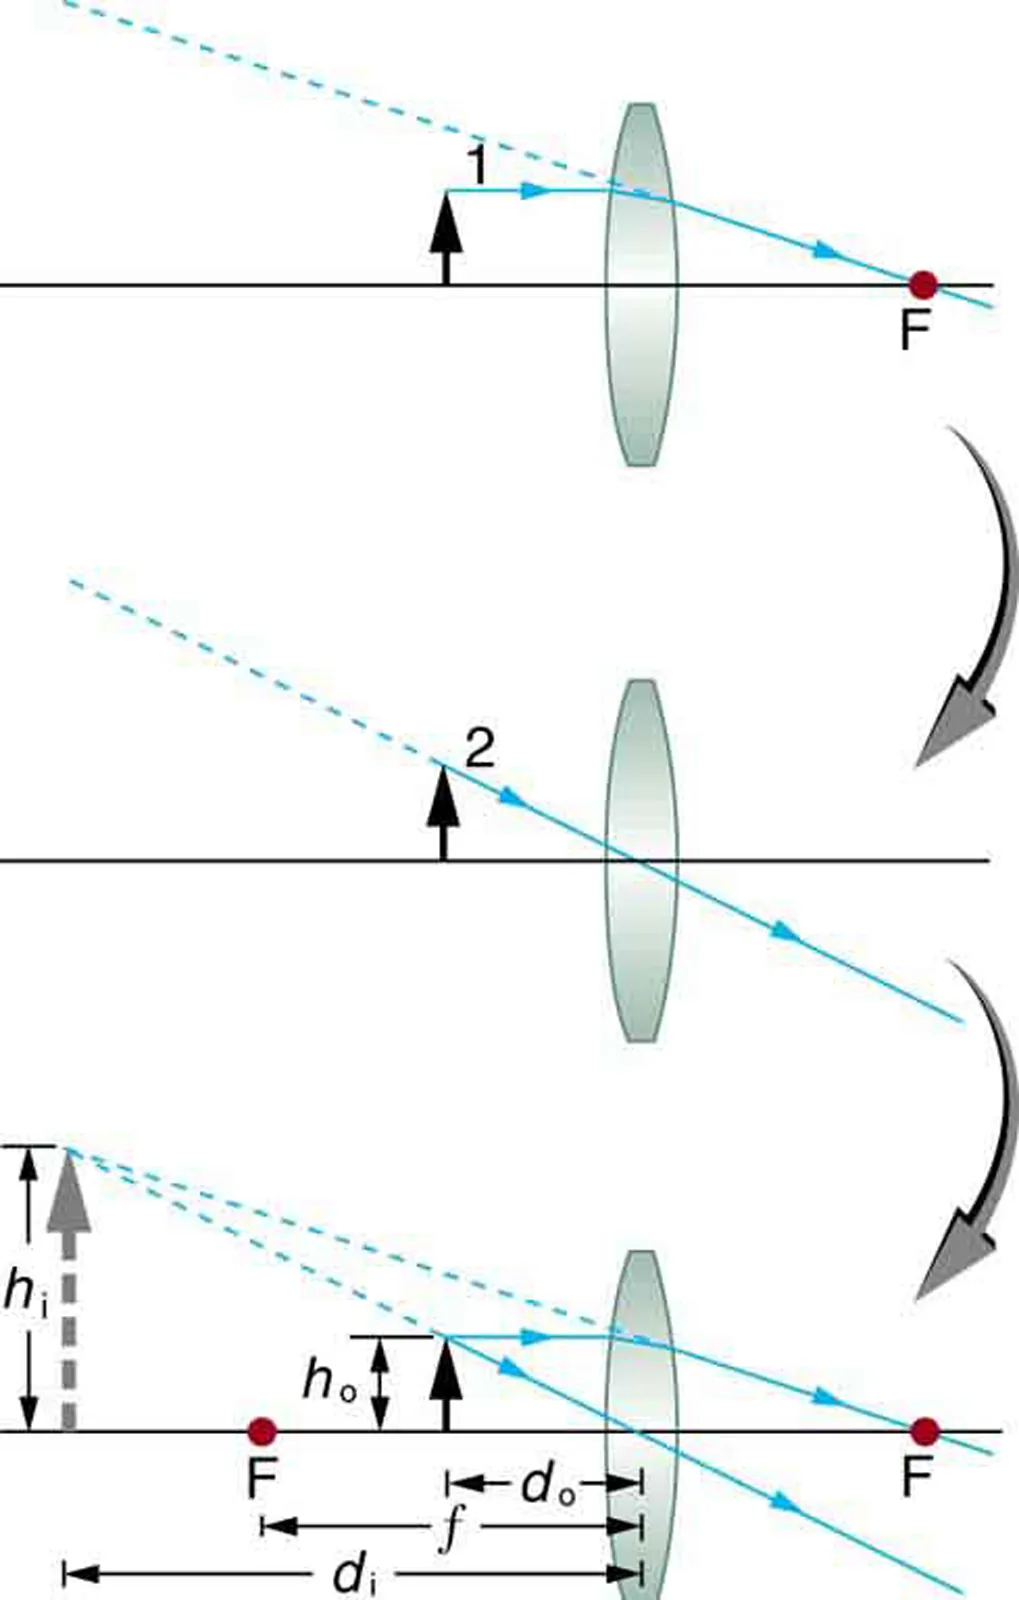
\includegraphics[width=0.75\textwidth]{figures/virtual.png}
%\caption{\label{fig:lens4} \footnotesize A \textbf{virtual image} forms if $d_o < f$.}
%\end{figure}
%\end{column}
%\begin{column}{0.5\textwidth}
%\textbf{Group exercise.} (a) Show that if $d_0 < f$, that $d_i < 0$.  (b) Show that the magnification is positive, and given by
%\begin{equation}
%m = \frac{f}{f-d_0}
%\end{equation}
%\textbf{Group exercise.} Design a magnifying glass (by solving for $f$) that gives $m = 10$ for an object 2.7 cm from the lens center.
%\end{column}
%\end{columns}
%\end{frame}
%
%\begin{frame}{Geometric optics: Lens optics}
%\small
%\textbf{\alert{Convex lenses}} create \textit{virtual images} when the object when $|d_0| > |f|$. 
%\begin{figure}
%\centering
%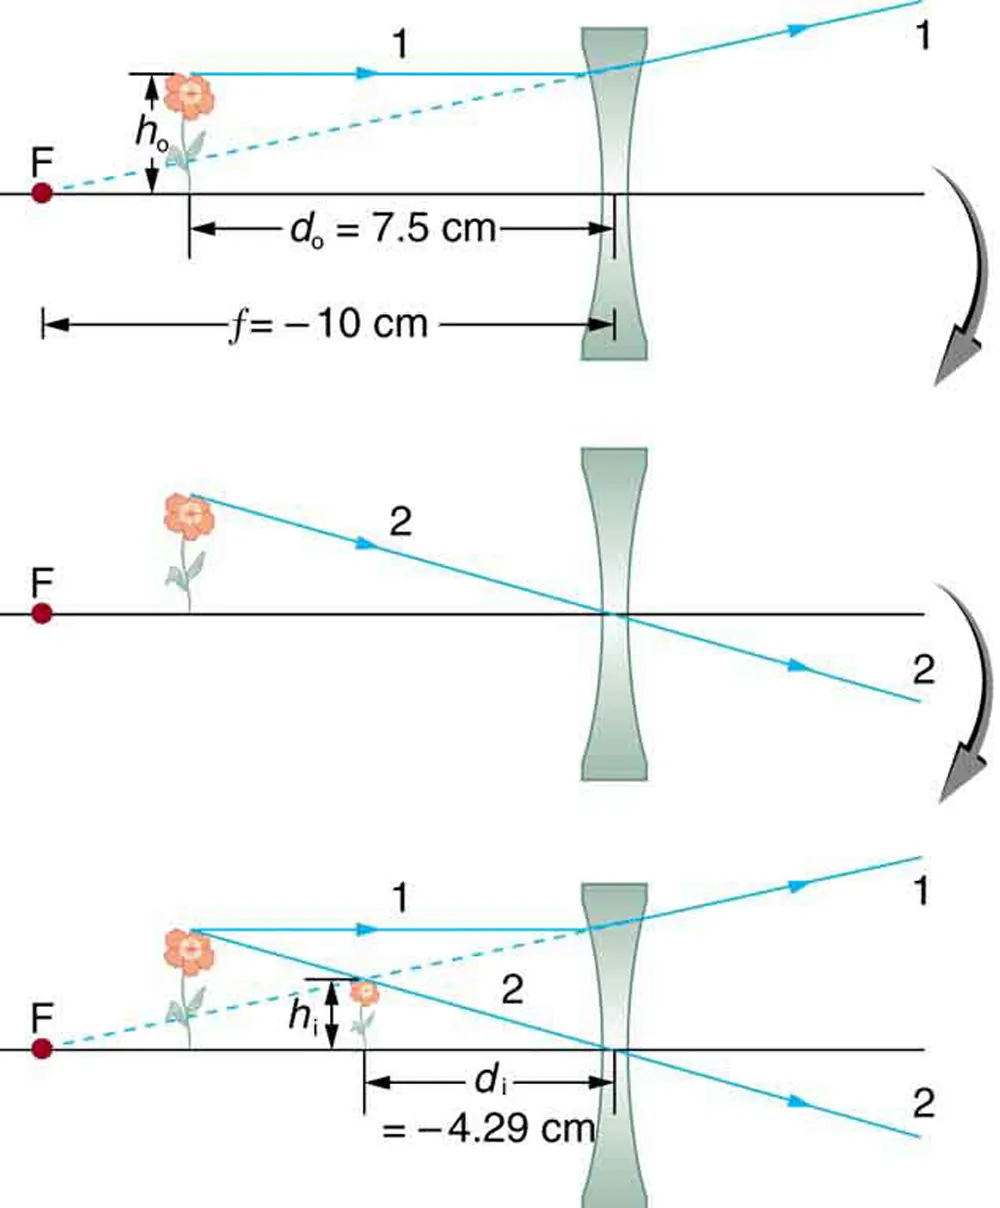
\includegraphics[width=0.45\textwidth]{figures/lens3.png}
%\caption{\label{fig:lens5} \small A convex lens diverges rays, and $f < 0$.}
%\end{figure}
%\end{frame}
%
%\begin{frame}{Geometric optics: Lens optics}
%\small
%Suppose an object such as a book page is held 7.50 cm from a concave lens of focal length –10.0 cm. Such a lens could be used in eyeglasses to correct pronounced nearsightedness. What magnification is produced?
%\begin{itemize}
%\item A: -0.57
%\item B: 4.2
%\item C: -4.2
%\item D: 0.57
%\end{itemize}
%\vspace{0.25cm}
%\textbf{\alert{Interesting final project idea:}} Measure the energy in sunlight by using a lens to concentrate sunlight to heat water by a fixed temperature.  For those interested in projects involving vision and medicine, see Chap. 26.
%\end{frame}
%
%\begin{frame}{Unit 5 Summary}
%\begin{enumerate}
%\item Electromagnetic waves - \textbf{Chapters 24.1 - 24.4}
%\begin{itemize}
%\item Maxwell's Equations
%\item Electromagnetic wave production
%\item Electromagnetic spectrum and energy
%\end{itemize}
%\item Geometric optics - \textbf{Chapters 25.1 - 25.3, 25.6}
%\begin{itemize}
%\item Ray-tracing and reflection
%\item Refraction
%\item Lens optics
%\end{itemize}
%\end{enumerate}
%\end{frame}
%
%\begin{frame}{Unit 5 Summary}
%\begin{enumerate}
%\item Wave optics - \textbf{Chapters 27.1 - 27.3}
%\begin{itemize}
%\item Wave interference
%\item Wave diffraction
%\item Double slit experiments
%\end{itemize}
%\item Nuclear physics in medicine - \textbf{32.1 - 32.4}
%\begin{itemize}
%\item Diagnostics and medical imaging
%\item Biological effects of ionizing radiation
%\item Therapeutic uses of ionizing radiation
%\item Food irradiation
%\end{itemize}
%\end{enumerate}
%\end{frame}
%
%\section{Wave optics: Wave interference and diffraction}
%
%\begin{frame}{Wave optics: Wave interference}
%\begin{columns}[T]
%\begin{column}{0.5\textwidth}
%\small
%\textbf{We observe} that light acts as a \textit{ray} and a \textit{wave.}
%\begin{itemize}
%\item Lasers are used for targeting in optical observatories, precisely because they travel in straight lines.
%\item When we pass lasers through \textit{diffraction gratings}, the light exhibits a \textit{diffraction pattern.} Rays don't diffract.
%\item $\lambda_n = \lambda/n$ in a medium with $n$.
%\end{itemize}
%\end{column}
%\begin{column}{0.5\textwidth}
%\begin{figure}
%\centering
%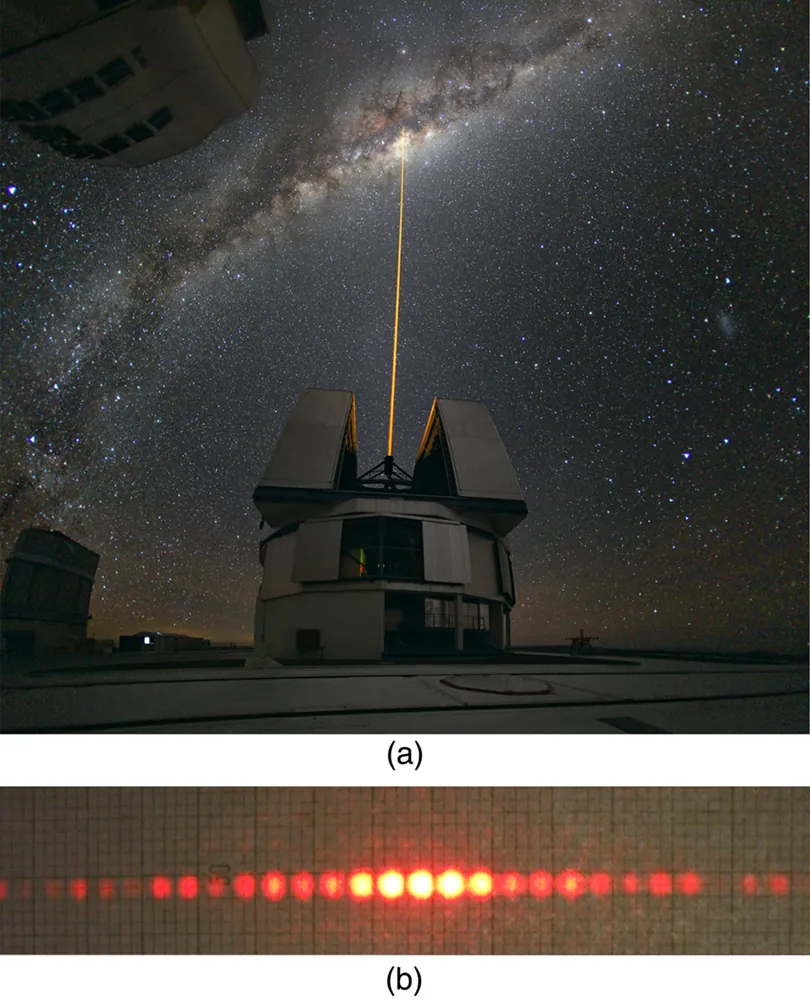
\includegraphics[width=0.85\textwidth]{figures/laser_wave.png}
%\caption{\label{fig:laser_wave} \footnotesize The Paranal Observatory of the ESO, in the Atacama Desert, Chile.}
%\end{figure}
%\end{column}
%\end{columns}
%\end{frame}
%
%\begin{frame}{Wave optics: Wave interference and diffraction}
%\begin{columns}[T]
%\begin{column}{0.5\textwidth}
%\small
%\textbf{We observe} that light acts as a \textit{ray} and a \textit{wave.}
%\begin{itemize}
%\item The 3D picture of an electromagnetic wave is that it is a wave in \textit{space} and \textit{time.}
%\item The electromagnetic wave also has lateral extent.
%\item \textit{Huygen's principle} states that every point along the wavefront is a point-source.
%\end{itemize}
%\end{column}
%\begin{column}{0.5\textwidth}
%\begin{figure}
%\centering
%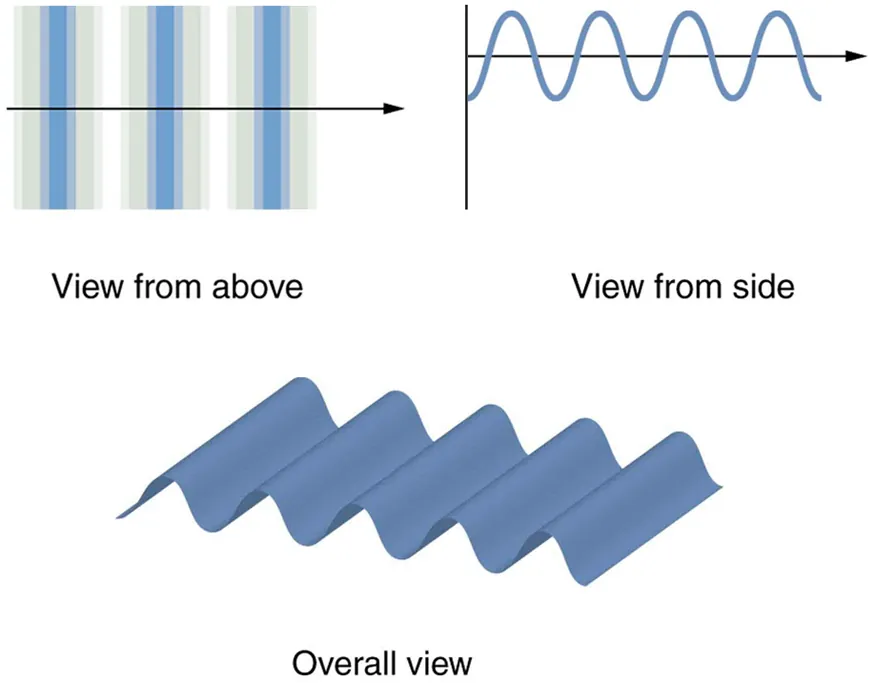
\includegraphics[width=0.85\textwidth]{figures/wave1.png}
%\caption{\label{fig:wave1} \footnotesize The three-dimensional picture of a transverse wave.}
%\end{figure}
%\end{column}
%\end{columns}
%\end{frame}
%
%\begin{frame}{Wave optics: Wave interference and diffraction}
%\begin{columns}[T]
%\begin{column}{0.5\textwidth}
%\small
%\textbf{We observe} that light acts as a \textit{ray} and a \textit{wave.}
%\begin{itemize}
%\item The 3D picture of an electromagnetic wave is that it is a wave in \textit{space} and \textit{time.}
%\item The electromagnetic wave also has lateral extent.
%\item \textit{Huygen's principle} states that every point along the wavefront is a point-source.
%\end{itemize}
%\end{column}
%\begin{column}{0.5\textwidth}
%\begin{figure}
%\centering
%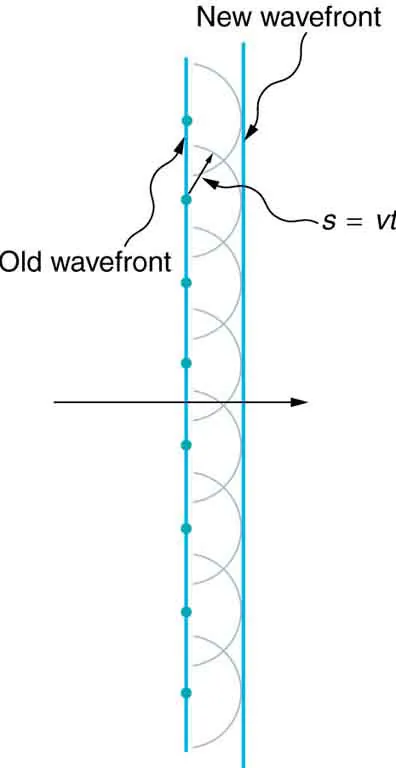
\includegraphics[width=0.55\textwidth]{figures/wave2.png}
%\caption{\label{fig:wave2} \footnotesize The three-dimensional picture of a transverse wave.}
%\end{figure}
%\end{column}
%\end{columns}
%\end{frame}
%
%\begin{frame}{Wave optics: Wave interference and diffraction}
%\begin{columns}[T]
%\begin{column}{0.5\textwidth}
%\small
%\textbf{We observe} that light acts as a \textit{ray} and a \textit{wave.}
%\begin{itemize}
%\item \textit{Huygen's principle} states that every point along the wavefront is a point-source.
%\item \textit{Huygen's principle} aligns with observations of specular reflection.
%\end{itemize}
%\end{column}
%\begin{column}{0.5\textwidth}
%\begin{figure}
%\centering
%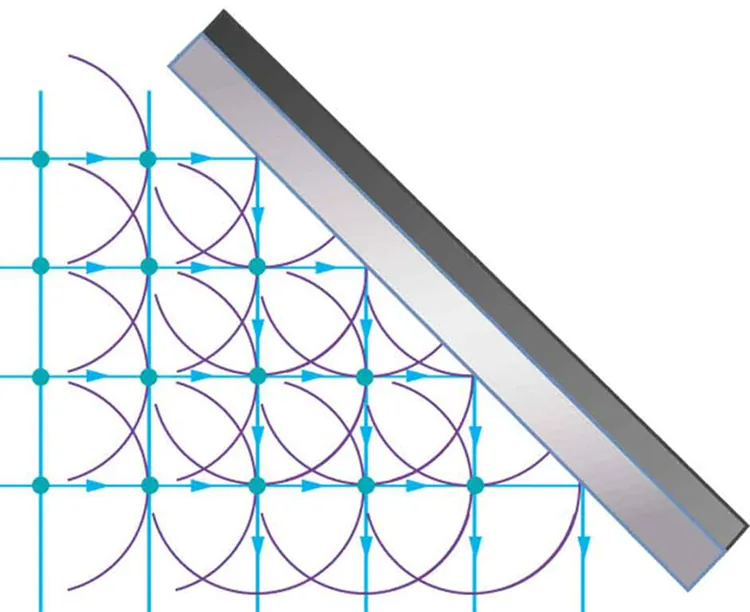
\includegraphics[width=0.75\textwidth]{figures/wave3.png}
%\caption{\label{fig:wave3} \footnotesize The transverse wave reflecting from a flat mirror.}
%\end{figure}
%\end{column}
%\end{columns}
%\end{frame}
%
%\begin{frame}{Wave optics: Wave interference and diffraction}
%\begin{columns}[T]
%\begin{column}{0.5\textwidth}
%\small
%\textbf{We observe} that light acts as a \textit{ray} and a \textit{wave.}
%\begin{itemize}
%\item \textit{Huygen's principle} states that every point along the wavefront is a point-source.
%\item \textit{Huygen's principle} aligns with observations of refraction between media with different indices of refraction.
%\item Notice that the wavelength changes, but the frequency does not.
%\end{itemize}
%\end{column}
%\begin{column}{0.5\textwidth}
%\begin{figure}
%\centering
%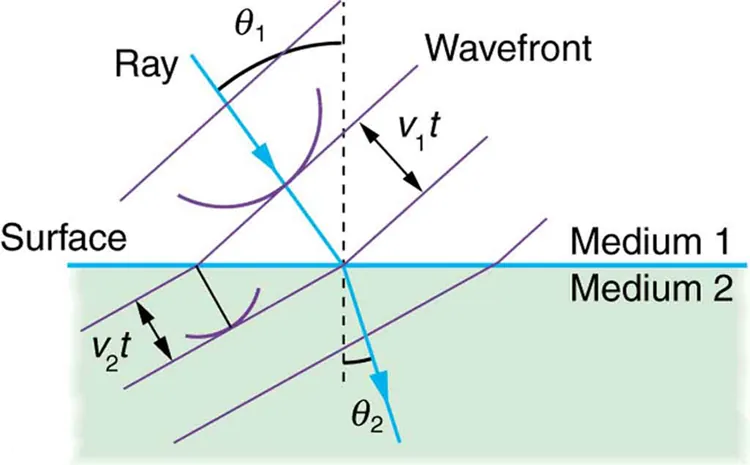
\includegraphics[width=0.95\textwidth]{figures/wave4.png}
%\caption{\label{fig:wave4} \footnotesize The transverse wave refracting into a medium with a new index of refraction.}
%\end{figure}
%\end{column}
%\end{columns}
%\end{frame}
%
%\begin{frame}{Wave optics: Wave interference and diffraction}
%\begin{columns}[T]
%\begin{column}{0.5\textwidth}
%\small
%\textbf{We observe} that light acts as a \textit{ray} and a \textit{wave.}
%\begin{itemize}
%\item \textit{Huygen's principle} states that every point along the wavefront is a point-source.
%\item \textit{Huygen's principle} aligns with observations of diffraction through openings that allow light (and sound) limited propagation.
%\end{itemize}
%\end{column}
%\begin{column}{0.5\textwidth}
%\begin{figure}
%\centering
%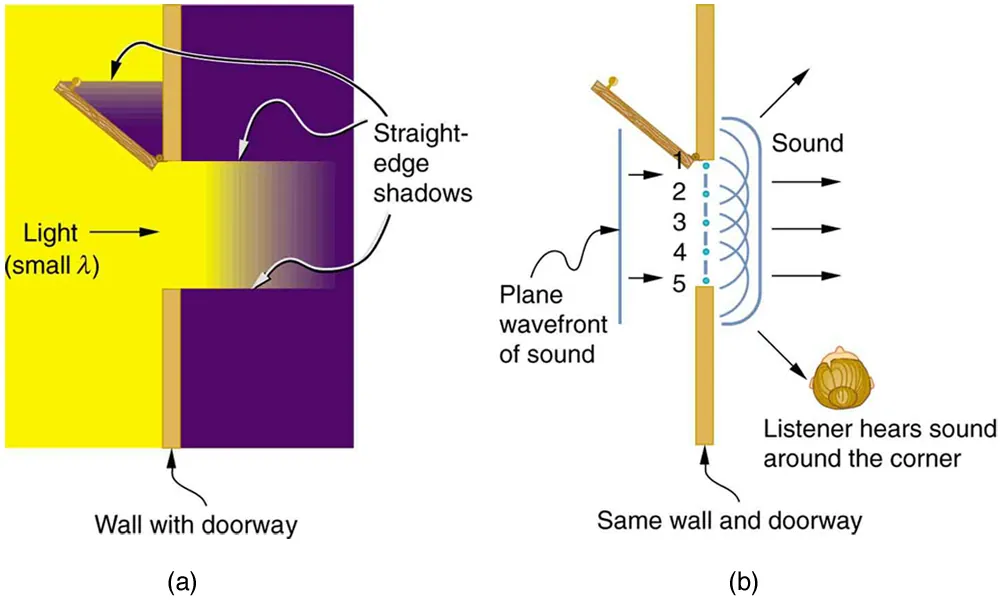
\includegraphics[width=0.95\textwidth]{figures/wave5.png}
%\caption{\label{fig:wave5} \footnotesize Light waves cause straight shadows, while sound waves diffract.  This is why you cannot see in the shadows, but you can hear sounds in another room.}
%\end{figure}
%\end{column}
%\end{columns}
%\end{frame}
%
%\begin{frame}{Wave optics: Wave interference and diffraction}
%\begin{columns}[T]
%\begin{column}{0.5\textwidth}
%\small
%\textbf{We observe} that light acts as a \textit{ray} and a \textit{wave.}
%\begin{itemize}
%\item \textit{Huygen's principle} states that every point along the wavefront is a point-source.
%\item \textit{Huygen's principle} aligns with observations of diffraction through openings that allow light (and sound) limited propagation.
%\item The key to diffraction is the comparison between wavelength, and length scale of the opening.
%\end{itemize}
%\end{column}
%\begin{column}{0.5\textwidth}
%\begin{figure}
%\centering
%\includegraphics[width=0.95\textwidth]{figures/wave6.png}
%\caption{\label{fig:wave6} \footnotesize Waves diffract more strongly through openings that are small compared to the wavelength.}
%\end{figure}
%\end{column}
%\end{columns}
%\end{frame}
%
%\section{Wave optics: Double slit experiments}
%
%\begin{frame}{Wave optics: Double slit experiments}
%\begin{columns}[T]
%\begin{column}{0.5\textwidth}
%\small
%\textbf{How do we prove that light is a wave?} Demonstrate the effects of \textit{constructive} and \textit{deconstructive} interference.
%\begin{itemize}
%\item \textit{Young's double-slit experiment.} In 1801, Thomas Young demonstrated that light exhibits constructive and deconstructive interference.
%\item The view of Isaac Newton and others was that light was a particle, and that there were other explanations of color and diffraction.
%\end{itemize}
%\end{column}
%\begin{column}{0.5\textwidth}
%\begin{figure}
%\centering
%\includegraphics[width=0.95\textwidth]{figures/slit1.png}
%\caption{\label{fig:slit1} \footnotesize If light is a particle, there should only be two slot images on the wall.}
%\end{figure}
%\end{column}
%\end{columns}
%\end{frame}
%
%\begin{frame}{Wave optics: Double slit experiments}
%\begin{columns}[T]
%\begin{column}{0.5\textwidth}
%\small
%\textbf{How do we prove that light is a wave?} Demonstrate the effects of \textit{constructive} and \textit{deconstructive} interference.
%\begin{itemize}
%\item \textit{Young's double-slit experiment.} In 1801, Thomas Young demonstrated that light exhibits constructive and deconstructive interference.
%\item Constructive and deconstructive interference occur when waves are in and out of phase, respectively.
%\end{itemize}
%\end{column}
%\begin{column}{0.5\textwidth}
%\begin{figure}
%\centering
%\includegraphics[width=0.75\textwidth]{figures/slit2.png}
%\caption{\label{fig:slit2} \footnotesize (a) Waves in phase add in amplitude. (b) Waves out of phase subtract in amplitude.}
%\end{figure}
%\end{column}
%\end{columns}
%\end{frame}
%
%\begin{frame}{Wave optics: Double slit experiments}
%\begin{columns}[T]
%\begin{column}{0.35\textwidth}
%\small
%\begin{itemize}
%\item The double-slit experiment creates two in-phase point sources, following Huygen's Principle.
%\item The two sources are separated by $d$ about the origin, and a screen is a distance $r \gg d$ from the origin.
%\end{itemize}
%\end{column}
%\begin{column}{0.65\textwidth}
%\begin{figure}
%\centering
%\includegraphics[width=0.95\textwidth]{figures/slit3.png}
%\caption{\label{fig:slit3} \footnotesize (a) A plane wave arrives at two slits. (b) A view of the wave magnitudes after the slits.  (c) The diffraction pattern on the screen.}
%\end{figure}
%\end{column}
%\end{columns}
%\end{frame}
%
%\section{PhET: Double slit experiments}
%
%\begin{frame}{Wave optics: Double slit experiments}
%\small
%Navigate to \url{https://phet.colorado.edu/en/simulations/wave-interference}.
%\footnotesize
%\begin{enumerate}
%\item \textbf{Waves tab learning goals:}
%\begin{itemize}
%\item Learn measurement controls
%\item Measure period, frequency, wavelength accurately
%\item Measure wave speed, and compare to $v = f\lambda$
%\item Perform measurements for water, sound, and light
%\end{itemize}
%\item \textbf{Interference tab learning goals:}
%\begin{itemize}
%\item Let $\theta_m$ be the angular location of constructive interference fringes.  Compare $d\sin\theta_m$ with $m\lambda$, where $m$ is an integer.
%\item Repeat this procedure with sound and light waves.
%\end{itemize}
%\end{enumerate}
%\end{frame}
%
%\begin{frame}{Wave optics: Double slit experiments}
%\small
%Navigate to \url{https://phet.colorado.edu/en/simulations/wave-interference}.
%\footnotesize
%\begin{enumerate}
%\item \textbf{Slits tab learning goals:}
%\begin{itemize}
%\item Repeat the procedure from the interference tab to show that the interference relationship is identical, provided certain criteria are met.
%\item Repeat this procedure with sound and light waves.
%\end{itemize}
%\item \textbf{Diffraction tab learning goals:}
%\begin{itemize}
%\item Explore the diffraction patterns of different combinations of boundary conditions and wavelengths.
%\item Explore the idea that the image we see is not necessarily the same as the shape of the source.
%\end{itemize}
%\end{enumerate}
%\end{frame}
%
%\begin{frame}{Wave optics: Double slit experiments}
%\footnotesize
%\begin{enumerate}
%\item \textbf{Waves tab learning goals:}
%\begin{itemize}
%\footnotesize
%\item Learn measurement controls.
%\begin{enumerate}
%\item Activate the water droplets with the green button.
%\item The color of the pool indicates wave amplitude.
%\item The frequency knob at right controls the drops per second.
%\item The amplitude knob controls the droplet size, and therefore wave amplitude.
%\end{enumerate}
%\item Measure period, frequency, wavelength accurately
%\begin{enumerate}
%\item Use the tape measure tool (upper right) to measure wavelength.
%\item Use the stopwatch and tape measure to measure wave speed ($\Delta x = v \Delta t$) as the waves proceed across the pool.
%\end{enumerate}
%\item Measure wave speed, and compare to $v = f\lambda$
%\begin{enumerate}
%\item Compare $v = \Delta x/\Delta t$ to $v = f\lambda$.  Do your results agree?
%\end{enumerate}
%\item Perform measurements for \textbf{\alert{water, sound, and light}}.
%\end{itemize}
%\end{enumerate}
%\end{frame}
%
%\begin{frame}{Wave optics: Double slit experiments}
%\footnotesize
%\begin{enumerate}
%\item \textbf{Interference tab learning goals:}
%\begin{itemize}
%\footnotesize
%\item Let $\theta_m$ be the angular location of constructive interference fringes.  Compare $d\sin\theta_m$ with $m\lambda$, where $m$ is an integer.
%\begin{enumerate}
%\item The source separation knob is on the right side.
%\item Allow the wave interference pattern to stabilize before measuring $\theta_m$, the angle between horizontal and the constructive interference fringe.
%\item Use the tape measure to measure the length of the hypoteneuse corresponding to the constructive interference fringe.  Also measure the distance to the edge of the pool.  Calculate $\theta_m$ using the appropriate trigonometric function.
%\item Adjust the controls to observe multiple fringes.  Compare $d\sin\theta$ to $m \lambda$, where $m$ is an integer.  Plot $d\sin\theta_m$ vs. $m\lambda$ while varying $\lambda$ (by changing the frequency).
%\end{enumerate}
%\item Repeat this procedure with \textbf{\alert{sound and light waves}}.
%\end{itemize}
%\end{enumerate}
%\end{frame}
%
%\begin{frame}{Wave optics: Double slit experiments}
%\footnotesize
%\begin{enumerate}
%\item \textbf{Slits tab learning goals:}
%\begin{itemize}
%\footnotesize
%\item \textbf{Repeat the procedure from the interference tab.}  Show that the interference relationship is identical, provided that the slit width is small compared to $\lambda$, and that the slit separation, $d$ is comparable to $\lambda$.
%\item Focus this procedure on \textbf{\alert{light waves}}.
%\item Create a graph of $d\sin\theta_1$ versus $m\lambda$, with $m = 1$, for 10-15 different optical wavelengths.
%\item Organize your data as follows: $\lambda$ in Column A, error or imprecision in $\lambda$ in Column B, $d\sin\theta_1$ in Column C, error or imprecision in $d\sin\theta_1$ in Column D.
%\item How do we calculate the propagated error in $d\sin\theta_1$?  Let $\sigma_f$ represent the error in this quantity.  Let $\sigma_\theta$ represent the error in $\theta$, and $\sigma_d$ represent the error in $d$.  The total error is
%\begin{equation}
%\sigma_f = \left(\sigma_d^2 \sin^2\theta + \sigma_\theta^2 d^2\cos^2\theta \right)^{1/2}
%\end{equation}
%\end{itemize}
%\end{enumerate}
%\end{frame}
%
%\begin{frame}{Wave optics: Double slit experiments}
%\footnotesize
%\begin{enumerate}
%\item \textbf{Diffraction tab learning goals:}
%\begin{itemize}
%\footnotesize
%\item Explore the diffraction patterns of different combinations of boundary conditions and wavelengths.
%\begin{enumerate}
%\item Start with the circle boundary.  Adjust the diameter to the largest setting (0.4 mm).
%\item Shrink the diameter to the smallest setting (0.04 mm) while leaving the wavelength constant.  Explain to your lab partner why the diffraction pattern morphs.  Compare this to the 1D case by using a 1 slit system in the \textbf{Slits Tab}, while adjusting the slit width.
%\end{enumerate}
%\item Explore the idea that the image we see is not necessarily the same as the shape of the source.
%\begin{enumerate}
%\item Now try different boundary conditions. In general, which direction (x or y) should be the \textit{longer} direction in the diffraction pattern, given your boundary conditions?
%\item Explain to your lab partner how the pattern is a result of \textit{Huygen's Principle.}
%\end{enumerate}
%\end{itemize}
%\end{enumerate}
%\end{frame}
%
%\begin{frame}{Wave optics: Double slit experiments}
%\begin{columns}[T]
%\begin{column}{0.5\textwidth}
%\small
%\textbf{\alert{Huygen's Principle}}, combined with the double-slit arrangement, shows the wave-like nature of light.
%\begin{itemize}
%    \item Mathematically, the \textit{far-field} approximation gives:
%    \begin{equation}
%        d\sin\theta = m\lambda
%    \end{equation}
%    \item Deconstructive interference occurs when:
%    \begin{equation}
%        d\sin\theta = \left(m + \frac{1}{2}\right)\lambda
%    \end{equation}
%\end{itemize}
%\end{column}
%\begin{column}{0.5\textwidth}
%\footnotesize
%\begin{figure}
%\centering
%\includegraphics[width=0.75\textwidth]{figures/slit4.png}
%\includegraphics[width=0.65\textwidth]{figures/slit5.png}
%\caption{\label{fig:slit4} \footnotesize For a path length difference of $(m+1/2)\lambda$, we observe a dark fringe.}
%\end{figure}
%\end{column}
%\end{columns}
%\end{frame}
%
%\begin{frame}{Wave optics: Double slit experiments}
%\begin{columns}[T]
%\begin{column}{0.5\textwidth}
%\small
%\textbf{\alert{Huygen's Principle}}, combined with the double-slit arrangement, shows the wave-like nature of light.
%\begin{itemize}
%    \item Mathematically, the \textit{far-field} approximation gives:
%    \begin{equation}
%        d\sin\theta = m\lambda
%    \end{equation}
%    \item Deconstructive interference occurs when:
%    \begin{equation}
%        d\sin\theta = \left(m + \frac{1}{2}\right)\lambda
%    \end{equation}
%\end{itemize}
%\end{column}
%\begin{column}{0.5\textwidth}
%\footnotesize
%\begin{figure}
%\centering
%\includegraphics[width=0.75\textwidth]{figures/slit6.png}
%\caption{\label{fig:slit5} \footnotesize The double-slit interference pattern depends on $\theta$ and $\lambda$.}
%\end{figure}
%\end{column}
%\end{columns}
%\end{frame}
%
%\begin{frame}{Wave optics: Double slit experiments}
%\begin{columns}[T]
%\begin{column}{0.5\textwidth}
%\footnotesize
%\begin{figure}
%\centering
%\includegraphics[width=0.55\textwidth]{figures/slit7.png}
%\caption{\label{fig:slit6} \footnotesize A repeated structure that affects light transmission is called a \textit{diffraction grating}.}
%\end{figure}
%\end{column}
%\begin{column}{0.5\textwidth}
%\footnotesize
%\begin{figure}
%\centering
%\includegraphics[width=0.75\textwidth]{figures/slit8.png}
%\caption{\label{fig:slit7} \footnotesize The diffraction pattern still retains peaks that correspond to integers $m$.}
%\end{figure}
%\end{column}
%\end{columns}
%\end{frame}
%
%\begin{frame}{Wave optics: Applications}
%\begin{figure}
%\centering
%\includegraphics[width=0.45\textwidth,trim=0cm 70cm 0cm 0cm,clip=true]{figures/grating.png}
%\includegraphics[width=0.45\textwidth]{figures/grating2.png}
%\caption{\label{fig:grating} \footnotesize The radiation pattern of a radar phased array design. (Left) Four diffraction patterns for 2.5 GHz radio waves.  (Right) Four diffraction patterns for 5.0 GHz radio waves.}
%\end{figure}
%\end{frame}
%
%\begin{frame}{Wave optics: Applications}
%\begin{figure}
%\centering
%\includegraphics[width=0.75\textwidth]{figures/slit10.png}
%\caption{\label{fig:grating2} \footnotesize The optical light reflected from gemstones and butterfly wings bears the signature of a diffraction grating that responds to the wavelength.}
%\end{figure}
%\end{frame}
%
%\begin{frame}{Unit 5 Summary}
%\begin{enumerate}
%\item Electromagnetic waves - \textbf{Chapters 24.1 - 24.4}
%\begin{itemize}
%\item Maxwell's Equations
%\item Electromagnetic wave production
%\item Electromagnetic spectrum and energy
%\end{itemize}
%\item Geometric optics - \textbf{Chapters 25.1 - 25.3, 25.6}
%\begin{itemize}
%\item Ray-tracing and reflection
%\item Refraction
%\item Lens optics
%\end{itemize}
%\end{enumerate}
%\end{frame}
%
%\begin{frame}{Unit 5 Summary}
%\begin{enumerate}
%\item Wave optics - \textbf{Chapters 27.1 - 27.3}
%\begin{itemize}
%\item Wave interference
%\item Wave diffraction
%\item Double slit experiments
%\end{itemize}
%\item Nuclear physics in medicine - \textbf{32.1 - 32.4}
%\begin{itemize}
%\item Diagnostics and medical imaging
%\item Biological effects of ionizing radiation
%\item Therapeutic uses of ionizing radiation
%\item Food irradiation
%\end{itemize}
%\end{enumerate}
%\end{frame}

\section{Nuclear physics in medicine: Introduction to Nuclear Isotopes and Radioactive Decay}

\begin{frame}{Introduction to Nuclear Isotopes and Radioactive Decay}
\footnotesize
One example of \textit{modern physics} deals with \textbf{\alert{radioactivity}}.  Radioactivity refers to the emission and detection of particles or radiation from \textbf{radioactive isotopes.}  THese are unstable nuclei that release energy in the form of radiation.
\begin{figure}
\centering
\includegraphics[width=0.75\textwidth]{figures/radioactivity.png}
\caption{\label{fig:radio} There are three basic types of radioactive decay: alpha particles, beta particles, and gamma particles.}
\end{figure}
\end{frame}

\begin{frame}{Introduction to Nuclear Isotopes and Radioactive Decay}
\small
\begin{columns}[T]
\begin{column}{0.5\textwidth}
\begin{table}
\centering
\begin{tabular}{| c | c | c |}
\hline
Type & Rest Mass & Charge \\ \hline
$\alpha$ & 3.727 GeV/c$^2$ & +2 \\ \hline
$\beta$ & 0.5111 MeV/c$^2$ & $\pm 1$ \\ \hline
$\gamma$ & 0 & 0 \\ \hline
\end{tabular}
\caption{\label{tab:radio} Radiation from nuclear decay is comprised of three particle types.}
\end{table}
Let $c$ be the speed of light, and let $E$ be the energy of a particle at rest.  Equation for the \textit{rest mass} of a sub-atomic or radioactive particle:
\begin{equation}
E = mc^2
\end{equation}
\end{column}
\begin{column}{0.5\textwidth}
The probability that \textbf{\alert{radioactivite particles}} penetrate biological tissue or matter depends on \textit{charge} and \textit{energy}.  One form of energy is the \textit{rest mass}, given by $E = mc^2$.
\begin{figure}
\centering
\includegraphics[width=0.95\textwidth]{figures/radioactivity.png}
\caption{\label{fig:radio2} There are three basic types of radioactive decay.}
\end{figure}
\end{column}
\end{columns}
\end{frame}

\begin{frame}{Introduction to Nuclear Isotopes and Radioactive Decay}
\begin{columns}[T]
\begin{column}{0.6\textwidth}
\footnotesize
\begin{table}
\centering
\begin{tabular}{| c | c | c |}
\hline
Type & Cross-section (b) & Energy (MeV) \\ \hline
$\alpha$ & $\approx 10^6$ & $\approx 4$ \\ \hline
$\beta$ & $\approx 1$ & $\approx 10$ \\ \hline
$\gamma$ & $\approx 0.2$ & $\approx 1$ \\ \hline
\end{tabular}
\caption{\label{tab:radio2} The \textbf{barn} is a unit of area, $10^{-24}$ cm$^2$.}
\end{table}
Let $I(z)$ be the intensity of a beam of particles traveling a distance $z$ through matter.  Let $n$ be the number density of atoms or scatterers in the matter.  Let $I_0$ be the original intensity.  The total cross-section $\sigma_{\rm tot}$ of the interactions relates these:
\begin{equation}
\boxed{I(z) = I_0 e^{-\sigma_{\rm tot} n z}}
\end{equation}
\end{column}
\begin{column}{0.4\textwidth}
\footnotesize
The probability that \textbf{\alert{radioactivite particles}} penetrate biological tissue or matter depends on the \textit{cross-section.}
\begin{figure}
\centering
\includegraphics[width=0.95\textwidth]{figures/radioactivity.png}
\caption{\label{fig:radio3} There are three basic types of radioactive decay.}
\end{figure}
\end{column}
\end{columns}
\end{frame}

\begin{frame}{Introduction to Nuclear Isotopes and Radioactive Decay}
\begin{columns}[T]
\begin{column}{0.6\textwidth}
\begin{equation}
I(z) = I_0 e^{-\sigma_{\rm tot} n z}
\end{equation}
Suppose a beam of radioactive decay products with total cross-section $\sigma_{\rm tot}$ is incident on a block of metal with number density $n$.  Show that half the intensity is gone at a distance $z_{\rm 1/2}$ into the metal, where
\begin{equation}
z_{\rm 1/2} = \frac{\ln 2}{\sigma n}
\end{equation}
\end{column}
\begin{column}{0.4\textwidth}
\footnotesize
Materials with higher density tend to block more radioactive decay products.
\begin{figure}
\centering
\includegraphics[width=0.95\textwidth]{figures/radioactivity.png}
\caption{\label{fig:radio4} There are three basic types of radioactive decay.}
\end{figure}
\end{column}
\end{columns}
\end{frame}

\begin{frame}{Introduction to Nuclear Isotopes and Radioactive Decay}
\begin{columns}[T]
\begin{column}{0.6\textwidth}
\small
\begin{equation}
z_{\rm 1/2} = \frac{\ln 2}{\sigma n}
\end{equation}
For lead, $n = 3.3 \times 10^{22}$ cm$^{-3}$, assuming 1 electron ready to scatter a $\gamma$-ray per nucleus.  If $\sigma = 1$ barn, $10^{-24}$ cm$^{2}$, how far in \textbf{lead} will the $\gamma$-rays travel before half of them are gone?
\begin{itemize}
\item A: 0.021 cm
\item B: 0.21 cm
\item C: 2.1 cm
\item D: 21 cm
\end{itemize}
\end{column}
\begin{column}{0.4\textwidth}
\footnotesize
Materials with higher density tend to block more radioactive decay products.
\begin{figure}
\centering
\includegraphics[width=0.95\textwidth]{figures/radioactivity.png}
\caption{\label{fig:radio5} The cross-section is related to how far a stream of particles will penetrate into a substance.}
\end{figure}
\end{column}
\end{columns}
\end{frame}

\begin{frame}{Introduction to Nuclear Isotopes and Radioactive Decay}
\begin{columns}[T]
\begin{column}{0.6\textwidth}
\small
Knowing that $z_{\rm 1/2}$ is inversely proportional to the cross-section, what would the result have been if the cross section was 1 Mb instead of 1 b?
\begin{itemize}
\item A: $2.1 \times 10^{-5}$ m
\item B: $2.1 \times 10^{-3}$ cm
\item C: $2.1 \times 10^{-5}$ cm
\item D: $2.1 \times 10^{-4}$ cm
\end{itemize}
\end{column}
\begin{column}{0.4\textwidth}
\footnotesize
Materials with higher density tend to block more radioactive decay products.
\begin{figure}
\centering
\includegraphics[width=0.95\textwidth]{figures/radioactivity.png}
\caption{\label{fig:radio6} Particles with smaller cross-sections penetrate much deeper into materials.}
\end{figure}
\end{column}
\end{columns}
\end{frame}

\begin{frame}{Introduction to Nuclear Isotopes and Radioactive Decay}
\begin{columns}[T]
\begin{column}{0.5\textwidth}
\small
The \textbf{\alert{half-life}} of a radioactive substance determines \textit{how long} it takes for the number of radioisotopes to reduce by half.
\begin{equation}
N(t) = N_{\rm 0} e^{-\lambda t}
\end{equation}
Show that the \textbf{half-life} is
\begin{equation}
t_{\rm 1/2} = \frac{\ln 2}{\lambda}
\end{equation}
The half-life of Carbon-14 is 5730 years, and Carbon 12 is the non-radioactive isotope.
\end{column}
\begin{column}{0.5\textwidth}
\begin{figure}
\centering
\includegraphics[width=0.95\textwidth]{figures/half-life.png}
\caption{\label{fig:radio7} Radioactive substances emit radiation, but have a finite amount of particles that can be radiated.}
\end{figure}
\end{column}
\end{columns}
\end{frame}

\begin{frame}{Introduction to Nuclear Isotopes and Radioactive Decay}
\begin{columns}[T]
\begin{column}{0.5\textwidth}
\small
\textbf{Group exercise:} Note that if we know the half-life value, $t_{\rm 1/2}$, we can get $\lambda$ from $\ln 2/\lambda$. Calculate the age of the Shroud of Turin given that the amount of Carbon-14 found in it is 92\% of that in living tissue.
\begin{enumerate}
\item Determine $\lambda$.
\item Note that $N/N_0 = 0.92$.
\item Solve for $t$.
\end{enumerate}
\end{column}
\begin{column}{0.5\textwidth}
\begin{figure}
\centering
\includegraphics[width=0.95\textwidth]{figures/half-life.png}
\caption{\label{fig:radio8} Given a finite amount of radioactive isotopes in a substance, and that decays are equally likely to occur in any given $\Delta t$, we can demonstrate exponential decay.}
\end{figure}
\end{column}
\end{columns}
\end{frame}

\begin{frame}{Introduction to Nuclear Isotopes and Radioactive Decay}
\begin{columns}[T]
\begin{column}{0.5\textwidth}
\small
\textbf{\alert{The decay rate}} can be derived from the $N(t)$ function:
\begin{align}
R &= \frac{\Delta N}{\Delta t} \\
R &=-\lambda N_0 e^{-\lambda t} \\
R &= -\left(\frac{\ln 2}{t_{\rm 1/2}}\right)N(t)
\end{align}
Intuitively, the \textit{decays per second} are proportional to the number of remaining radioactive isotopes, $N$, and inversely proportional to the half-life.  The SI unit of radioactive decay is the \textbf{becquerel}, or 1 decay/second.
\end{column}
\begin{column}{0.5\textwidth}
\begin{figure}
\centering
\includegraphics[width=0.95\textwidth]{figures/half-life.png}
\caption{\label{fig:radio9} It takes about 10 half-lives to decay $10^6$ isotopes.}
\end{figure}
\end{column}
\end{columns}
\end{frame}

\section{Nuclear physics in medicine: Diagnostics and medical imaging}

\begin{frame}{Nuclear physics in medicine: Diagnostics and medical imaging}
\textbf{Nuclear physics}, encompassing radioactive isotopes and radiation, is used in medicine. \\ \vspace{0.5cm}
\small
Consider the \textit{radioimmunoassay} (RIA) technique.
\begin{enumerate}
\item Irradiate a sample of antigen with a radioactive isotope so that the nuclei in the substance become radioactive.
\item Mix with a sample from a patient containing unknown number of antigens.
\item Introduce antibodies that bind to the antigen.
\item Separate bound and unbound antigens.
\item Measure decay rate of unbound antigens.
\item Work out the answer.
\end{enumerate}
\end{frame}

\begin{frame}{Nuclear physics in medicine: Diagnostics and medical imaging}
\textbf{Nuclear physics}, encompassing radioactive isotopes and radiation, is used in medicine. \\ \vspace{0.5cm}
\small
Consider an analogy, to measure the number of fish in a pond:
\begin{enumerate}
\item Catch, tag, and release $n$ fish, in a pond with unknown number of fish $N$.
\item Return to the pond, and catch $m$ fish.
\item Count the \textit{untagged fish}, $m_u$.  $(m_u + m_t = m)$.
\item Assert that the uncaught fraction is a constant, $f = m_u/m = (N-n)/N$
\item Work out the answer:
\begin{equation}
N = \frac{n}{1-f}
\end{equation}
\end{enumerate}
\end{frame}

\begin{frame}{Nuclear physics in medicine: Diagnostics and medical imaging}
\textbf{Nuclear physics}, encompassing radioactive isotopes and radiation, is used in medicine. \\ \vspace{0.5cm}
\small
Consider an analogy, to measure the number of fish in a pond:
\begin{enumerate}
\item Catch, tag, and release $n$ fish, in a pond with unknown number of fish $N$.
\item Return to the pond, and catch $m$ fish.
\item Count the \textit{untagged fish}, $m_u$.  $(m_u + m_t = m)$.
\item Assert that the uncaught fraction is a constant, $f = m_u/m = (N-n)/N$
\item Work out the answer:
\begin{equation}
N = \frac{n}{1-f}
\end{equation}
\end{enumerate}
\end{frame}

\begin{frame}{Nuclear physics in medicine: Diagnostics and medical imaging}
\textbf{Nuclear physics}, encompassing radioactive isotopes and radiation, is used in medicine. \\ \vspace{0.5cm}
\small
\begin{equation}
N = \frac{n}{1-f}
\end{equation}
If we tag $n = 67$ fish, and our untagged fraction is $f = 0.33$, how many fish are in the pond?
\begin{itemize}
\item A: 10
\item B: 67
\item C: 100
\item D: 133
\end{itemize}
\end{frame}

\begin{frame}{Introduction to Nuclear Isotopes and Radioactive Decay}
\begin{columns}[T]
\begin{column}{0.5\textwidth}
\small
How do we measure \textbf{\alert{radioactively tagged}} molecules?
\end{column}
\begin{column}{0.5\textwidth}
\begin{figure}
\centering
\includegraphics[width=0.95\textwidth]{figures/anger_camera.png}
\caption{\label{fig:medicine_1} An gamma camera, or Anger camera.}
\end{figure}
\end{column}
\end{columns}
\end{frame}

\section{Nuclear physics in medicine: Biological effects of ionizing radiation}

\section{Nuclear physics in medicine: Therapeutic uses of ionizing radiation}

\section{Nuclear physics in medicine: Food irradiation}

\section{Conclusion}

\begin{frame}{Unit 5 Summary}
\begin{enumerate}
\item Electromagnetic waves - \textbf{Chapters 24.1 - 24.4}
\begin{itemize}
\item Maxwell's Equations
\item Electromagnetic wave production
\item Electromagnetic spectrum and energy
\end{itemize}
\item Geometric optics - \textbf{Chapters 25.1 - 25.3, 25.6}
\begin{itemize}
\item Ray-tracing and reflection
\item Refraction
\item Lens optics
\end{itemize}
\end{enumerate}
\end{frame}

\begin{frame}{Unit 5 Summary}
\begin{enumerate}
\item Wave optics - \textbf{Chapters 27.1 - 27.3}
\begin{itemize}
\item Wave interference
\item Wave diffraction
\item Double slit experiments
\end{itemize}
\item Nuclear physics in medicine - \textbf{32.1 - 32.4}
\begin{itemize}
\item Diagnostics and medical imaging
\item Biological effects of ionizing radiation
\item Therapeutic uses of ionizing radiation
\item Food irradiation
\end{itemize}
\end{enumerate}
\end{frame}

\end{document}
